\documentclass[lang=cn,12pt,scheme=chinese]{elegantbook}

\title{数学分析(B2)课程讲义}

\bioinfo{简介}{
    本讲义为汪琥庭老师2024秋季学期数学分析B2课程讲义的latex整理版,不包括复习课内容.
}
\date{\today}
\version{2.0}
\author{助教 刘越}

\setcounter{tocdepth}{3}
\cover{cover.jpg}

\extrainfo{\bfseries 本讲义仅供学习交流使用,未经许可请勿用于商业目的.\\
如有错误或疏漏请联系邮箱:\url{liuyue22@ustc.mail.edu.cn}\\
\href{https://passiflora-sago.github.io/24FallMAB2.html}{课程主页} \quad
\href{https://github.com/Passiflora-sago/Passiflora-sago.github.io/releases/download/v1.0.0/maexams_2025-v1.pdf}{往年卷汇总}}


% 本文档命令
\usepackage{array}
\newcommand{\ccr}[1]{\makecell{{\color{#1}\rule{1cm}{1cm}}}}

% 修改标题页的橙色带
\definecolor{customcolor}{RGB}{32,178,170}
\colorlet{coverlinecolor}{customcolor}
\usepackage{cprotect}

\addbibresource[location=local]{reference.bib} % 参考文献,不要删除

%# -*- coding: utf-8 -*-

% preamble_command_mathematics_v1_0.tex

% ---------- macro definition ----------
% ----- equation setting -----
\everymath{\displaystyle}

% ----- command -----
\newcommand{\les}{\leqslant}
\newcommand{\ges}{\geqslant}
\newcommand{\degree}{^{\circ}}
\newcommand{\circA}{\overset{\circ}{\mathrm{A}}}
\newcommand{\dageq}{\stackrel{\dag}{ = }}
\newcommand{\ddageq}{\stackrel{\ddag}{ = }}
\newcommand{\dbdageq}{\stackrel{\dbdag}{ = }}
\newcommand{\stareq}{\stackrel{*}{ = }}
\newcommand{\dagiff}{\stackrel{\dag}{\iff}}
\newcommand{\ddagiff}{\stackrel{\ddag}{\iff}}
\newcommand{\dagimp}{\stackrel{\dag}{\implies}}
\newcommand{\ddagimp}{\stackrel{\ddag}{\implies}}
\newcommand{\tensor}[1]{\overleftrightarrow{#1}}
% \renewcommand\tensor[1]{\overset{\scriptscriptstyle\leftrightarrow}{#1}}
\renewcommand{\tensor}[1]{\overset{\scriptstyle\leftrightarrow}{#1}}
\newcommand{\by}{\leftarrow}

\newcommand{\join}{\Join}

% \renewcommand\pi{\piup}
\newcommand{\PI}{\uppi}
% \renewcommand\pi{\uppi}
% \renewcommand\pi{\text{\textpi}}
% \renewcommand\pi{\textrm{\greektext p}}

\newcommand{\nimplies}{\centernot\implies}
\newcommand{\nimpliedby}{\centernot\impliedby}

\renewcommand{\Re}{\mathrm{Re}\,}
\renewcommand{\Im}{\mathrm{Im}\,}
\newcommand{\const}{\mathrm{Const.}}
\newcommand{\sym}{\mathrm{sym}}
\newcommand{\cyc}{\mathrm{cyc}}
\newcommand{\ii}{\,\mathrm{i}}
\newcommand{\jj}{\,\mathrm{j}}

\DeclareMathOperator{\sgn}{sgn}
\DeclareMathOperator{\dif}{d\!}
\DeclareMathOperator{\diff}{d}
\DeclareMathOperator{\trans}{T}
\DeclareMathOperator{\tr}{tr}
\DeclareMathOperator{\grad}{\mathbf{grad}}
\DeclareMathOperator{\rank}{rank}
\DeclareMathOperator{\diag}{diag}
\DeclareMathOperator{\sinc}{sinc}
\DeclareMathOperator{\ad}{ad}
\DeclareMathOperator{\ex}{E}
\DeclareMathOperator{\var}{Var}
\DeclareMathOperator{\argmin}{arg\,min}
\DeclareMathOperator{\argmax}{arg\,max}
\DeclareMathOperator{\softmax}{softmax}
\DeclareMathOperator{\arccot}{arccot}
\DeclareMathOperator{\st}{s.t.}
\DeclareMathOperator{\iid}{i.i.d.}
\DeclareMathOperator{\Exp}{Exp}
\DeclareMathOperator{\Poi}{Poi}

\renewcommand{\parallel}{/\!\!/}

\newcommand{\bR}{\bm{\mathcal{R}}}

\newcommand{\Alpha}{\mathrm{A}}
\newcommand{\Beta}{\mathrm{B}}
\newcommand{\Epsilon}{\mathrm{E}}

\newcommand{\rA}{\mathrm{A}}
\newcommand{\rB}{\mathrm{B}}
\newcommand{\rC}{\mathrm{C}}
\newcommand{\rD}{\mathrm{D}}
\newcommand{\rE}{\mathrm{E}}
\newcommand{\rF}{\mathrm{F}}
\newcommand{\rG}{\mathrm{G}}
\newcommand{\rH}{\mathrm{H}}
\newcommand{\rI}{\mathrm{I}}
\newcommand{\rJ}{\mathrm{J}}
\newcommand{\rK}{\mathrm{K}}
\newcommand{\rL}{\mathrm{L}}
\newcommand{\rM}{\mathrm{M}}
\newcommand{\rN}{\mathrm{N}}
\newcommand{\rO}{\mathrm{O}}
\newcommand{\rP}{\mathrm{P}}
\newcommand{\rQ}{\mathrm{Q}}
\newcommand{\rR}{\mathrm{R}}
\newcommand{\rS}{\mathrm{S}}
\newcommand{\rT}{\mathrm{T}}
\newcommand{\rU}{\mathrm{U}}
\newcommand{\rV}{\mathrm{V}}
\newcommand{\rW}{\mathrm{W}}
\newcommand{\rX}{\mathrm{X}}
\newcommand{\rY}{\mathrm{Y}}
\newcommand{\rZ}{\mathrm{Z}}
\newcommand{\ra}{\mathrm{a}}
\newcommand{\rb}{\mathrm{b}}
\newcommand{\rc}{\mathrm{c}}
\newcommand{\rd}{\mathrm{d}}
\newcommand{\re}{\mathrm{e}}
\newcommand{\rf}{\mathrm{f}}
\newcommand{\rg}{\mathrm{g}}
\newcommand{\rh}{\mathrm{h}}
\newcommand{\ri}{\mathrm{i}}
\newcommand{\rj}{\mathrm{j}}
\newcommand{\rk}{\mathrm{k}}
\newcommand{\rl}{\mathrm{l}}
\renewcommand{\rm}{\mathrm{m}}
\newcommand{\rn}{\mathrm{n}}
\newcommand{\ro}{\mathrm{o}}
\newcommand{\rp}{\mathrm{p}}
\renewcommand{\rq}{\mathrm{q}}
\newcommand{\rr}{\mathrm{r}}
\newcommand{\rs}{\mathrm{s}}
\newcommand{\rt}{\mathrm{t}}
\newcommand{\ru}{\mathrm{u}}
\newcommand{\rv}{\mathrm{v}}
\newcommand{\rw}{\mathrm{w}}
\newcommand{\rx}{\mathrm{x}}
\newcommand{\ry}{\mathrm{y}}
\newcommand{\rz}{\mathrm{z}}

\newcommand{\0}{\bm{0}}
\newcommand{\1}{\bm{1}}
\newcommand{\A}{\bm{A}}
\newcommand{\B}{\bm{B}}
\newcommand{\C}{\bm{C}}
\newcommand{\D}{\bm{D}}
\newcommand{\E}{\bm{E}}
\newcommand{\F}{\bm{F}}
\newcommand{\G}{\bm{G}}
\renewcommand{\H}{\bm{H}}
\newcommand{\I}{\bm{I}}
\newcommand{\J}{\bm{J}}
\newcommand{\K}{\mathbb{K}}
\renewcommand{\L}{\bm{L}}
\newcommand{\M}{\bm{M}}
\newcommand{\N}{\mathbb{N}}
\renewcommand{\O}{\bm{O}}
\renewcommand{\P}{\bm{P}}
\newcommand{\Q}{\mathbb{Q}}
\newcommand{\R}{\mathbb{R}}
\renewcommand{\S}{\bm{S}}
\newcommand{\T}{\bm{T}}
\newcommand{\U}{\bm{U}}
\newcommand{\V}{\bm{V}}
\newcommand{\W}{\bm{W}}
\newcommand{\X}{\bm{X}}
\newcommand{\Y}{\bm{Y}}
\newcommand{\Z}{\mathbb{Z}}
\renewcommand{\a}{\bm{a}}
\renewcommand{\b}{\bm{b}}
\renewcommand{\c}{\bm{c}}
\renewcommand{\d}{\bm{d}}
\newcommand{\e}{\mathrm{e}}
\newcommand{\f}{\bm{f}}
\newcommand{\g}{\bm{g}}
\newcommand{\h}{\bm{h}}
\renewcommand{\i}{\bm{i}}
\renewcommand{\j}{\bm{j}}
\renewcommand{\k}{\bm{k}}
\renewcommand{\l}{\bm{l}}
\newcommand{\m}{\bm{m}}
\newcommand{\n}{\bm{n}}
\renewcommand{\o}{\bm{o}}
\newcommand{\p}{\bm{p}}
\newcommand{\q}{\bm{q}}
% \renewcommand\r{\bm{r}}
\newcommand{\br}{\bm{r}}
\newcommand{\s}{\bm{s}}
\renewcommand{\t}{\bm{t}}
\renewcommand{\u}{\bm{u}}
\renewcommand{\v}{\bm{v}}
\newcommand{\w}{\bm{w}}
\newcommand{\x}{\bm{x}}
\newcommand{\y}{\bm{y}}
\newcommand{\z}{\bm{z}}

\newcommand{\balpha}{\bm{\alpha}}
\newcommand{\bbeta}{\bm{\beta}}
\newcommand{\bchi}{\bm{\chi}}
\newcommand{\bdelta}{\bm{\delta}}
\newcommand{\bvarepsilon}{\bm{\varepsilon}}
\newcommand{\bphi}{\bm{\phi}}
\newcommand{\bvarphi}{\bm{\varphi}}
\newcommand{\bgamma}{\bm{\gamma}}
\newcommand{\bmeta}{\bm{\eta}}
\newcommand{\biota}{\bm{\iota}}
\newcommand{\bkappa}{\bm{\kappa}}
\newcommand{\blambda}{\bm{\lambda}}
\newcommand{\bvarLambda}{\bm{\varLambda}}
\newcommand{\bmu}{\bm{\mu}}
\newcommand{\bnu}{\bm{\nu}}
\newcommand{\bpi}{\bm{\pi}}
\newcommand{\bvarpi}{\bm{\varpi}}
\newcommand{\btheta}{\bm{\theta}}
\newcommand{\bvartheta}{\bm{\vartheta}}
\newcommand{\brho}{\bm{\rho}}
\newcommand{\bsigma}{\bm{\sigma}}
\newcommand{\bvarsigma}{\bm{\varsigma}}
\newcommand{\btau}{\bm{\tau}}
\newcommand{\bupsilon}{\bm{\upsilon}}
\newcommand{\bomega}{\bm{\omega}}
\newcommand{\bxi}{\bm{\xi}}
\newcommand{\bpsi}{\bm{\psi}}
\newcommand{\bzeta}{\bm{\zeta}}
\newcommand{\bAlpha}{\bm{\Alpha}}
\newcommand{\bBeta}{\bm{\Beta}}
\newcommand{\bChi}{\bm{\Chi}}
\newcommand{\bDelta}{\bm{\Delta}}
\newcommand{\bEpsilon}{\bm{\Epsilon}}
\newcommand{\bPhi}{\bm{\Phi}}
\newcommand{\bGamma}{\bm{\Gamma}}
\newcommand{\bEta}{\bm{\Eta}}
\newcommand{\bIota}{\bm{\Iota}}
\newcommand{\bKappa}{\bm{\Kappa}}
\newcommand{\bLambda}{\bm{\Lambda}}
\newcommand{\bMu}{\bm{\Mu}}
\newcommand{\bNu}{\bm{\Nu}}
\newcommand{\bPi}{\bm{\Pi}}
\newcommand{\bTheta}{\bm{\Theta}}
\newcommand{\bRho}{\bm{\Rho}}
\newcommand{\bSigma}{\bm{\Sigma}}
\newcommand{\bvarSigma}{\bm{\varSigma}}
\newcommand{\bTau}{\bm{\Tau}}
\newcommand{\bUpsilon}{\bm{\Upsilon}}
\newcommand{\bOmega}{\bm{\Omega}}
\newcommand{\bXi}{\bm{\Xi}}
\newcommand{\bPsi}{\bm{\Psi}}
\newcommand{\bZeta}{\bm{\Zeta}}
\newcommand{\ve}{\varepsilon}
\newcommand{\laplace}{\Delta}

% 启用 expl3 语法处理多个变量
\ExplSyntaxOn

% 定义 \parfrac 宏,默认阶数为 1,支持多个变量
\NewDocumentCommand{\parfrac}{O{1} m m}
{
  \frac{
    \int_compare:nNnTF {#1} = {1} {\partial #2} {\partial^{#1} #2}
  }
  {
    \parfrac_process_vars:n { #3 }
  }
}

% 处理逗号分隔的多个偏导变量
\cs_new_protected:Nn \parfrac_process_vars:n
{
  \seq_set_split:Nnn \l_tmpa_seq { , } { #1 }
  \seq_map_inline:Nn \l_tmpa_seq { \partial ##1 }
}

\ExplSyntaxOff

\definecolor{structurecolor}{RGB}{60,113,183}
\definecolor{main}{RGB}{76,141,174}
\definecolor{second}{RGB}{213,180,92}
\definecolor{third}{RGB}{120,146,98}




\begin{document}
\maketitle
\frontmatter

\tableofcontents
\mainmatter

\chapter{三维向量的五种运算}

\section{三维直角坐标系与三维向量的线性运算}

\begin{definition}[空间直角坐标系]
    从空间一点$O$出发,作三条两两垂直(正交)的射线,并确定单位与方向,构成$O-xyz$直角坐标系.
\end{definition}


\begin{proposition}
    \begin{enumerate}
        \item $xOy$坐标面,$zOy$坐标面,$zOx$坐标面两两正交并将整个空间分割成八个卦限.
        \item 点$M$:设$M$为空间任一点,过$M$点分别作$Ox$,$Oy$,$Oz$轴的垂面.可得三个垂足$A$,$B$,$C$,设$A$,$B$,$C$代表的实数为$a$,$b$,$c$.则点,则点$M$与有序数组$(a,b,c)$一一对应,记作$M(a,b,c)$.坐标原点为$O(0,0,0)$.
        \item 向量$\overrightarrow{OM}$:在$Ox$,$Oy$,$Oz$轴正向上分别取三个单位向量$\i,\j,\k$,则$\overrightarrow{OA}=a\i$, $\overrightarrow{OB}=b\j$,$\overrightarrow{OC}=c\k$,依照平面向量的加法法则(平行四边形法则,三角形法则)$\overrightarrow{OM}=\overrightarrow{ON}+\overrightarrow{OC}=\overrightarrow{OA}+\overrightarrow{OB}+\overrightarrow{OC}=a\i+b\j+c\k\triangleq(a,b,c)$.同时可得$\i=(1,0,0),\j=(0,1,0),\k=(0,0,1)$,零向量$\0=(0,0,0)$.
        \item 如上定义的$M$,$\overrightarrow{OM}$与有序数组$(a,b,c)$一一对应.
        \item $\i\bot\j$,$\i\bot\k$,$\j\bot\k$.
    \end{enumerate}

\end{proposition}

\begin{figure}[h]
    \centering
    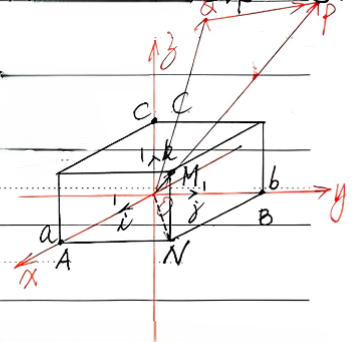
\includegraphics[width=0.5\textwidth]{figure/1-1空间直角坐标系.png}
    \caption{空间直角坐标系}
    \label{fig:fig1}
\end{figure}

\begin{definition}
    $\overrightarrow{OM}=(a,b,c)$,称$\sqrt{a^2+b^2+c^2}$为向量$\overrightarrow{OM}$的模,记为$\left|\overrightarrow{OM}\right|$.

    模长为$0$的向量为零向量$\0=(0,0,0)$,模长为$1$的向量称为单位向量.
\end{definition}
\begin{proposition}
    设向量$\balpha=(a,b,c)\neq \0$,则$\left|\balpha\right|\neq 0$.
    
    此时,$\balpha^0\triangleq\frac{\balpha}{\left|\balpha\right|}=\left(\frac{a}{\sqrt{a^2+b^2+c^2}},\frac{b}{\sqrt{a^2+b^2+c^2}},\frac{c}{\sqrt{a^2+b^2+c^2}}\right)$是单位向量.
\end{proposition}


\begin{remark}
\begin{enumerate}
    \item 这种定义方式较为依赖直观的几何性质,且可能存在一些循环定义的问题,当然针对这一阶段这样大概就足够了.
    \item 这种方式可以想见,是可以从三维向量(three-dimensional vector)推广至$n$维的,对应的向量就是$n$维向量(n-dimensional vector).
\end{enumerate}
\end{remark}
设$P=(x_1,y_1,z_1),Q=(x_1,y_1,z_1)$是空间的任意两点,$\overrightarrow{OP}=(x_1,y_1,z_1)$,$\overrightarrow{OQ}=(x_2,y_2,z_2)$.则$\overrightarrow{PQ}=(x_2,y_2,z_2)-(x_1,y_1,z_1)=(x\i+x_2\j+z_2\k)-(x_1\i+y_1\j+z_1\k)=(x_2-x_1)\i+(y_2-y_1)\j+(z_2-z_1)\k=(x_2-x_1,y_2-y_1,z_2-z_1)$.
即空间的任一个向量$\overrightarrow{PQ}=(x_2-x_1,y_2-y_1,z_2-z_1)$.

空间中的向量有无数个,但每一个都可用单位向量$\i,\j,\k$的线性组合来表示,称之前定义的$\i,\j,\k$为三维向量空间的标准正交基.

在任一个有限维的向量空间中,一旦选定了基向量,则"无限的问题便可有限化表示"了.

\begin{proposition}[三维数组向量的线性运算法则]
    设$\balpha=(a_1,b_1,c_1),\bbeta=(a_2,b_2,c_2),\lambda_1\in\R,\lambda_2\in\R$,则
    \begin{enumerate}
        \item 加、减法:$\balpha\pm\bbeta=(a_1\i+b_1\j+c_1\k)\pm(a_2\i+b_2\j+c_2\k)=(a_1\pm a_2)\i+(b_1\pm b_2)\j+(c_1\pm c_2)\k=(a_1\pm a_2,b_1\pm b_2,c_1\pm c_2)$.
        \item 数乘:$\lambda_1\balpha=\lambda_1(a_1\i+b_1\j+c_1\k)=(\lambda_1a_1)\i+(\lambda_1b_1)\j+(\lambda_1c_1)\k=(\lambda_1a_1,\lambda_1b_1,\lambda_1c_1)$.
    \end{enumerate}
    向量的加法、减法及数乘三种运算统称为向量的线性运算.统一为
    
    $\lambda_1\balpha+\lambda_2\bbeta=(\lambda_1a_1,\lambda_1b_1,\lambda_1c_1)+(\lambda_2a_2,\lambda_2b_2,\lambda_2c_2)=(\lambda_1a_1+\lambda_2a_2,\lambda_1b_1+\lambda_2b_2,\lambda_1c_1+\lambda_2c_2)$.
\end{proposition}

\section{向量的内积与外积}
\begin{definition}[内积与外积]
    设$\balpha=(a_1,b_1,c_1),\bbeta=(a_2,b_2,c_2)$.则
    \begin{enumerate}
        \item 内积: $\balpha\cdot\bbeta=\left|\balpha\right|\left|\bbeta\right|\cos(\widehat{\balpha,\bbeta})$
        \item 外积: $\balpha\times\bbeta$,满足$\begin{cases}
            \left|\balpha\times\bbeta\right|=\left|\balpha\right|\left|\bbeta\right|\sin(\widehat{\balpha,\bbeta})\\
            \balpha\times\bbeta\bot\balpha,\balpha\times\bbeta\bot\bbeta,\text{且}\balpha,\bbeta,\balpha\times\bbeta\text{构成右手系}.
        \end{cases}$
    \end{enumerate}
\end{definition}

\begin{figure}[h]
    \centering
    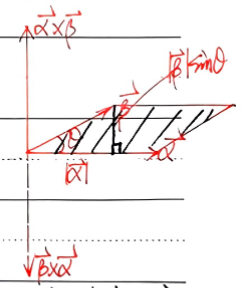
\includegraphics[width=0.5\textwidth]{figure/1-2外积的图示.png}
    \caption{外积的图示}
    \label{fig:fig2}
\end{figure}
\begin{remark}
    \begin{enumerate}
        \item $\balpha\cdot\bbeta$的规定来源于物理中里做功的运算,$\balpha\cdot\bbeta$是一个数,故称内积$\balpha\cdot\bbeta$为$\balpha$与$\bbeta$的数量积,或者称为点乘.
        \item $\balpha\times\bbeta$的规定来源于物理中的力矩的运算,$\balpha\times\bbeta$是一个向量,故称外积$\balpha\times\bbeta$为$\balpha$与$\bbeta$的向量积,或者称为叉乘.
    \end{enumerate}
\end{remark}

\begin{theorem}
    \begin{enumerate}
        \item $\balpha\bot\bbeta\Leftrightarrow\balpha\cdot\bbeta=0\Leftrightarrow a_1a_2+b_1b_2+c_1c_2=0$.
        \item $\balpha\parallel\bbeta\Leftrightarrow\balpha\times\bbeta=\0\Leftrightarrow\frac{a_1}{a_2}=\frac{b_1}{b_2}=\frac{c_1}{c_2}\Leftrightarrow \balpha=\lambda\bbeta$
    \end{enumerate}
\end{theorem}
\begin{proof}
    \begin{enumerate}
        \item 
        \begin{enumerate}[1)]
            \item 若$\balpha\bot\bbeta$,则$\cos(\widehat{\balpha,\bbeta})=0\Rightarrow\balpha\cdot\bbeta=\left|\balpha\right|\left|\bbeta\right|\cos(\widehat{\balpha,\bbeta})=0$.            
            \item 反之,若$\balpha\cdot\bbeta=0$,则$\left|\balpha\right|\left|\bbeta\right|\cos(\widehat{\balpha,\bbeta})=0$,若$\left|\balpha\right|\left|\bbeta\right|\neq 0$,则$\cos(\widehat{\balpha,\bbeta})=0$,从而$\balpha\bot\bbeta$.若$\left|\balpha\right|\left|\bbeta\right|=0$,则$\balpha=\0$或$\bbeta=\0$,由于零向量$\0$垂直于任意向量,故$\balpha\bot\bbeta$.
            \item $\balpha\cdot\bbeta=(a_1\i+b_1\j+c_1\k)\cdot(a_2\i+b_2\j+c_2\k)=a_1a_2\i\cdot\i+a_1b_2\i\cdot\j+a_1c_2\i\cdot\k+b_1a_2\j\cdot\i+b_1b_2\j\cdot\j+b_1c_2\j\cdot\k+c_1a_2\k\cdot\i+c_1b_2\k\cdot\j+c_1c_2\k\cdot\k.\text{而}\i\cdot\i=\left|\i\right|\left|\i\right|\cos(\widehat{\i,\i})=1\times1\times\cos0=1=\j\cdot\j=\k\cdot\k,\text{且由于}\i\bot\j,\i\bot\k,\j\bot\k,\text{故}\i\cdot\j=\i\cdot\k=\j\cdot\k=0,\text{故}\balpha\cdot\bbeta=a_1a_2+b_1b_2+c_1c_2$.
        \end{enumerate}
        \item
        \begin{enumerate}[1)]
            \item 若$\balpha\parallel\bbeta$,则$\sin(\widehat{\balpha,\bbeta})=0\Rightarrow\left|\balpha\times\bbeta\right|=\left|\balpha\right|\left|\bbeta\right|\sin(\widehat{\balpha,\bbeta})=0\Rightarrow\balpha\times\bbeta=\0$.
            \item 反之,若$\balpha\times\bbeta=\0$,则$\left|\balpha\times\bbeta\right|=\left|\0\right|=0=\left|\balpha\right|\left|\bbeta\right|\sin(\widehat{\balpha,\bbeta})$,若$\left|\balpha\right|\left|\bbeta\right|\neq 0$,则$\sin(\widehat{\balpha,\bbeta})=0$,从而$\balpha\parallel\bbeta$.若$\left|\balpha\right|\left|\bbeta\right|=0$,则$\balpha=\0$或$\bbeta=\0$,由于零向量$\0$平行于任意向量,故$\balpha\parallel\bbeta$.
            \item $
            \begin{cases}
                \i\times\i=\0,\j\times\j=\0,\k\times\k=\0\\
                \i\times\j=\k,\j\times\i=-\k,\j\times\k=\i\\
                \k\times\j=-\i,\k\times\i=\j,\i\times\k=-\j
            \end{cases}$
            $\Rightarrow \balpha\times\bbeta=(a_1\i+b_1\j+c_1\k)\times(a_2\i+b_2\j+c_2\k)=a_1a_2\i\times\i+a_1b_2\i\times\j+a_1c_2\i\times\k+b_1a_2\j\times\i+b_1b_2\j\times\j+b_1c_2\j\times\k+c_1a_2\k\times\i+c_1b_2\k\times\j+c_1c_2\k\times\k=a_1b_2\k-a_1c_2\j-b_1a_2\k+b_1c_2\i+c_1a_2\j-c_1b_2\i=(b_1c_2-c_1b_2)\i-(a_1c_2-c_1a_2)\j+(a_1b_2-b_1a_2)\k=\begin{matrix}
                \begin{vmatrix}
                    \i&\j&\k\\
                    a_1&b_1&c_1\\
                    a_2&b_2&c_2
                \end{vmatrix}
            \end{matrix}$.
            由$bf{\alpha}\parallel\bbeta\Leftrightarrow\balpha\times\bbeta=\0=(0,0,0)\Leftrightarrow\begin{cases}
                b_1c_2-c_1b_2=0\\
                c_1a_2-a_1c_2=0\\
                a_1b_2-b_1a_2=0
            \end{cases}
            \Leftrightarrow \frac{a_1}{a_2}=\frac{b_1}{b_2}=\frac{c_1}{c_2}\triangleq\lambda$.
            因此可得$\balpha=\lambda\bbeta$.
        \end{enumerate}
    \end{enumerate}
\end{proof}
\begin{remark}
    \begin{enumerate}
        \item 在上述证明中,不加证明地使用了点乘与叉乘的分配率等性质.
        \item 与证明中提到的类似,点乘有坐标表达$\balpha\cdot\bbeta=a_1a_2+b_1b_2+c_1c_2$,叉乘有坐标表达$\balpha\times\bbeta=\begin{matrix}
            \begin{vmatrix}
                \i&\j&\k\\
                a_1&b_1&c_1\\
                a_2&b_2&c_2
            \end{vmatrix}\end{matrix}$,     
        这也是最常用的计算公式.
    \end{enumerate}
\end{remark}

\section{例题}
    设$\balpha=(a_1,b_1,c_1),\bbeta=(a_2,b_2,c_2),\bgamma=(a_3,b_3,c_3)$.
\begin{example}
    证明:柯西不等式$\left|a_1a_2+b_1b_2+c_1c_2\right|\les\sqrt{a_1^2+b_1^2+c_1^2}\sqrt{a_2^2+b_2^2+c_2^2}$.
\end{example}

\begin{proof}
    $\left|a_1a_2+b_1b_2+c_1c_2\right|=\left|\balpha\cdot\bbeta\right|=\left|\balpha\right|\left|\bbeta\right|\cos(\widehat{\balpha,\bbeta})\les\left|\balpha\right|\left|\bbeta\right|=\sqrt{a_1^2+b_1^2+c_1^2}\sqrt{a_2^2+b_2^2+c_2^2}$.
\end{proof}

\begin{remark}
    在$n$维向量空间中,设$\balpha=(a_1,a_2,\cdots,a_n),\bbeta=(b_1,b_2,\cdots,b_n)$,则$\left|\balpha\cdot\bbeta\right|=\left|\balpha\right|\left|\bbeta\right|\cos(\widehat{\balpha,\bbeta})\les\left|\balpha\right|\left|\bbeta\right|$,即$\left|a_1b_1+a_2b_2+\cdots+a_nb_n\right|\les\sqrt{a_1^2+a_2^2+\cdots+a_n^2}\sqrt{b_1^2+b_2^2+\cdots+b_n^2}$.
\end{remark}

\begin{example}
    证明:$\left|\balpha\times\bbeta\right|^2=\left|\balpha\right|^2\left|\bbeta\right|^2-\left|\balpha\cdot\bbeta\right|^2$.
\end{example}
\begin{proof}
    $\left|\balpha\times\bbeta\right|^2=\left|\balpha\right|^2\left|\bbeta\right|^2\sin^2(\widehat{\balpha,\bbeta})=\left|\balpha\right|^2\left|\bbeta\right|^2(1-\cos^2(\widehat{\balpha,\bbeta}))=\left|\balpha\right|^2\left|\bbeta\right|^2-\left|\balpha\right|^2\left|\bbeta\right|^2\cos^2(\widehat{\balpha,\bbeta})=\left|\balpha\right|^2\left|\bbeta\right|^2-\left|\balpha\cdot\bbeta\right|^2$.
\end{proof}

\begin{example}
    证明:$(\balpha\times\bbeta)\cdot\bgamma=(\bbeta\times\bgamma)\cdot\balpha=(\bgamma\times\balpha)\cdot\bbeta$.
\end{example}
\begin{proof}
    $(\balpha\times\bbeta)\cdot\bgamma=\begin{matrix}
        \begin{vmatrix}
            \i&\j&\k\\
            a_1&b_1&c_1\\
            a_2&b_2&c_2
        \end{vmatrix}
    \end{matrix}\cdot(a_3\i+b_3\j+c_3\k)=((b_1c_2-c_1b_2)\i+(c_1a_2-a_1c_2)\j+(a_1b_2-a_2b_1)\k)\cdot(a_3\i+b_3\j+c_3\k)=(b_1c_2-c_1b_2)a_3+(c_1a_2-a_1c_2)b_3+(a_1b_2-a_2b_1)c_3=\begin{matrix}
        \begin{vmatrix}
            a_1&b_1&c_1\\
            a_2&b_2&c_2\\
            a_3&b_3&c_3
        \end{vmatrix}
    \end{matrix}=(\bbeta\times\bgamma)\cdot\balpha=(\bgamma\times\balpha)\cdot\bbeta$.
\end{proof}

\begin{example}
    证明:三个向量$\balpha,\bbeta,\bgamma$共面的充要条件是$(\balpha\times\bbeta)\cdot\bgamma=0$.
\end{example}
\begin{proof}
    是如下结论的结果:如图所示,根据计算公式,$\left|\balpha\times\bbeta\right|$是以$\balpha$和$\bbeta$为两边的平行四边形的面积,而$\bgamma\left|\cos(\widehat{\balpha\times\bbeta,\bgamma})\right|$是$\bgamma$在垂直于平行四边形方向上的投影,即$h=\left|\bgamma\right|\left|\cos(\widehat{\balpha\times\bbeta,\bgamma})\right|$,因此$(\balpha\times\bbeta)\cdot\bgamma$是以$\balpha$, $\bbeta$和$\bgamma$为三边的平行六面体的体积,于是$\balpha,\bbeta,\bgamma$共面$\Leftrightarrow$平行六面体的体积为$0$ $\Leftrightarrow(\balpha\times\bbeta)\cdot\bgamma=\begin{matrix}
        \begin{vmatrix}
            a_1&b_1&c_1\\
            a_2&b_2&c_2\\
            a_3&b_3&c_3
        \end{vmatrix}
    \end{matrix}=0$.
\end{proof}

\begin{figure}[h]
    \centering
    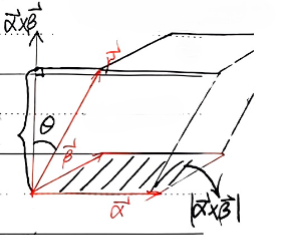
\includegraphics[width=0.5\textwidth]{figure/1-3混合积与平行六面体.png}
    \caption{混合积与平行六面体}
    \label{fig:fig3}
\end{figure}
\begin{example}
    $\forall \lambda_1,\lambda_2\in\R$总有$\balpha,\bbeta,\lambda_1\balpha+\lambda_2\bbeta$共面.
\end{example}
\begin{proof}
    利用$\balpha\bot\balpha\times\bbeta,\bbeta\bot\balpha\times\bbeta$,则$(\balpha\times\bbeta)\cdot\balpha=0,(\balpha\times\bbeta)\cdot\bbeta=0$,从而$(\balpha\times\bbeta)\cdot(\lambda_1\balpha+\lambda_2\bbeta)=0$,因此可得$\balpha,\bbeta,\lambda_1\balpha+\lambda_2\bbeta$共面.
\end{proof}

\begin{homework} 
    ex8.1:6,9,10,12,14,17,23,26.
\end{homework}
\chapter{空间平面与直线}

\section{平面(plane)的五种表示形式}

\begin{definition}[平面的五种表示形式]
    \begin{enumerate}
        \item 向量式:设平面$\pi$过已知点$M_0(x_0,y_0,z_0)$,且与已知的非零向量$\n=(A,B,C)$垂直,则平面$\pi$唯一确定.设$P(x,y,z)$为$\pi$上任一点,则有$\overrightarrow{M_0P}\bot\n$,于是有$$\n\cdot \overrightarrow{M_0P}=0$$称为平面$\pi$的向量式方程.
        \item 点法式:由向量式,有$\n\cdot \overrightarrow{M_0P}=0$,即$$A(x-x_0)+B(y-y_0)+C(z-z_0)=0$$,称为平面$\pi$的向量式方程.
        \item 一般式:设$D=-Ax_0-By_0-Cz_0$,则有$$Ax+By+Cz+D=0$$称为平面$\pi$的一般式方程.
        \item 截距式:一般式中,设$d\triangleq-D\neq 0$,令$\frac{d}{A}=a,\frac{d}{B}=b,\frac{d}{C}=c$,则$$\frac{x}{a}+\frac{y}{b}+\frac{z}{c}=1$$称为平面$\pi$的截距式方程.
        \item 三点式:设$A(x_1,y_1,z_1),B(x_2,y_2,z_2),C(x_3,y_3,z_3)$为$\pi$上不共线的三点,则由$A,B,C$三点确定唯一的平面$\pi$,设$P(x,y,z)$为$\pi$上任一点,则有$\overrightarrow{AP},\overrightarrow{AB},\overrightarrow{AC}$共面,即$$\begin{vmatrix}x-x_1&y-y_1&z-z_1\\x_2-x_1&y_2-y_1&z_2-z_1\\x_3-x_1&y_3-y_1&z_3-z_1\end{vmatrix}=0$$称为平面$\pi$的三点式方程.
    \end{enumerate}
\end{definition}

\section{空间直线(line)的五种表示形式}
\begin{definition}[空间直线的五种表示形式]
    \begin{enumerate}
        \item 向量式:设直线$l$过已知点$M_0(x_0,y_0,z_0)$,且与已知的非零向量$\btau=(l,m,n)$平行,则直线$l$唯一确定.设$P(x,y,z)$为$l$上任一点,则有$\overrightarrow{M_0P}\parallel\n$,于是有$$\overrightarrow{M_0P}\times\btau=\0$$称为直线$l$的向量式方程.
        \item 点向式:由向量式,有$\overrightarrow{M_0P}\parallel\btau$,则有$$\frac{x-x_0}{l}=\frac{y-y_0}{m}=\frac{z-z_0}{n}$$,称为直线$l$的点向式方程.
        \item 参数式,在点向式中,令$\frac{x-x_0}{l}=\frac{y-y_0}{m}=\frac{z-z_0}{n}=t$,则有$$\begin{cases}x=x_0+lt\\y=y_0+mt\\z=z_0+nt\end{cases}$$称为直线$l$的参数式方程.
        \item 交面式:设平面$p_1:A_1x+B_1y+C_1z+D_1=0$和平面$p_2:A_2x+B_2y+C_2z+D_2=0$不平行,则$\pi_1$与$\pi_2$有交线$l$,$l$上的点$P(x,y,z)$满足$$\begin{cases}A_1x+B_1y+C_1z+D_1=0\\A_2x+B_2y+C_2z+D_2=0\end{cases}$$称为直线$l$的交面式方程.
        \item 两点式:设$Q_1(x_1,y_1,z_1),Q_2(x_2,y_2,z_2)$为直线$l$上的两点,则由$Q_1,Q_2$确定唯一的直线$l$,设$P(x,y,z)$为$l$上任一点,则有$\overrightarrow{Q_1P},\overrightarrow{Q_1Q_2}$共线,即$$\frac{x-x_1}{x_2-x_1}=\frac{y-y_1}{y_2-y_1}=\frac{z-z_1}{z_2-z_1}$$称为直线$l$的两点式方程.   
    \end{enumerate}
\end{definition}
\newpage
\section{面面,线线,线面之间的关系}
\begin{proposition}
    设$$\begin{cases}
        \pi_1:A_1x+B_1y+C_1z+D_1=0,&\n_1=(A_1,B_1,C_1)\\
        \pi_2:A_2x+B_2y+C_2z+D_2=0,&\n_2=(A_2,B_2,C_2)\\
        L_1:\frac{x-x_1}{l_1}=\frac{y-y_1}{m_1}=\frac{z-z_1}{n_1},&\btau_1=(l_1,m_1,n_1)\\
        L_2:\frac{x-x_2}{l_2}=\frac{y-y_2}{m_2}=\frac{z-z_2}{n_2},&\btau_2=(l_2,m_2,n_2)
    \end{cases}$$
    则\begin{enumerate}
        \item $\pi_1\parallel\pi_2\Leftrightarrow\frac{A_1}{A_2}=\frac{B_1}{B_2}=\frac{C_1}{C_2}\Leftrightarrow\n_1\times\n_2=\0$.
        \item $\pi_1\bot\pi_2\Leftrightarrow A_1A_2+B_1B_2+C_1C_2=0\Leftrightarrow\n_1\cdot\n_2=0$.
        \item $\pi_1$与$\pi_2$的夹角$\alpha(0<\alpha\les\pi),\cos\alpha=\frac{\n_1\cdot\n_2}{\left|\n_1\right|\cdot\left|\n_2\right|}=\n_1^0\cdot\n_2^0$,即得$\alpha=\arccos\frac{\n_1\cdot\n_2}{\left|\n_1\right|\cdot\left|\n_2\right|}$.
        \item $L_1\parallel L_2\Leftrightarrow\btau\parallel\btau_2\Leftrightarrow\btau_1\times\btau_2=\0\Leftrightarrow\frac{l_1}{l_2}=\frac{m_1}{m_2}=\frac{n_1}{n_2}$.
        \item $L_1\bot L_2\Leftrightarrow\btau_1\bot\btau_2\Leftrightarrow\btau_1\cdot\btau_2=0\Leftrightarrow l_1l_2+m_1m_2+n_1n_2=0$.
        \item $L_1$与$L_2$的夹角$\alpha(0\les\alpha\les\pi),\cos\alpha=\frac{\btau_1\cdot\btau_2}{\left|\btau_1\right|\cdot\left|\btau_2\right|}=\btau_1^0\cdot\btau_2^0$,即得$\alpha=\arccos\frac{\btau_1\cdot\btau_2}{\left|\btau_1\right|\cdot\left|\btau_2\right|}$.
        \item $L_1\bot\pi_1\Leftrightarrow\btau_1\parallel\n_1\Leftrightarrow\btau_1\times\n_1=\0\Leftrightarrow \frac{A_1}{l_1}=\frac{B_1}{m_1}=\frac{C_1}{n_1}$.
        \item $L_1\parallel\pi_1\Leftrightarrow\btau_1\bot\n_1\Leftrightarrow\btau_1\cdot\n_1=0\Leftrightarrow A_1l_1+B_1m_1+C_1n_1=0$.
        \item $L_1$与$\pi_1$的夹角$\beta(0\les\beta\les\frac{\pi}{2}),\cos(\frac{\pi}{2}-\beta)=\left|\frac{\btau_1\cdot\n_1}{\left|\btau_1\right|\cdot\left|\n_1\right|}\right|=\left|\btau_1^0\cdot\n_1^0\right|$,故$\sin\beta=\left|\btau_1^0\cdot\n_1^0\right|0$,即得$\beta=\arcsin\left|\btau_1^0\cdot\n_1^0\right|$.
    \end{enumerate}
\end{proposition}

\section{例题}
\begin{example}
    分别求已知点$M(1,-1,-2)$关于点$A(1,0,1)$,平面$\pi:3x+4y-5z-1=0$,直线$L:\frac{x-1}{-1}=\frac{y-1}{2}=\frac{z-1}{0}$的对称点$Q(x,y,z)$.
\end{example}
\begin{solution}
    \begin{enumerate}
        \item $A(1,0,1)$是线段$MQ$的中点,有$\begin{cases}\frac{1+x}{2}=1\\y=\frac{-1+y}{2}=0\\z=\frac{-2+z}{2}=1\end{cases}\Rightarrow\begin{cases}x=1\\y=1\\z=4\end{cases}$,即$Q(1,1,4)$.
        \item $\n=(3,4,-5)$,则有$\begin{cases}\overrightarrow{MQ}\parallel\n\\MQ\text{中点}N(\frac{x+1}{2},\frac{y-1}{2},\frac{z-2}{2})\text{在}\pi\text{上} \end{cases}$
        
        $\Rightarrow\begin{cases}x=1+3t\\y=-1+4t\\z=-2-5t\\3(\frac{x+1}{2})+4(\frac{y-1}{2})-5\frac{z-2}{2}-1=0\end{cases}$
        
        $\Rightarrow t=\frac{12}{25}$,带回$x,y,z$可知$Q(\frac{61}{25},\frac{23}{25},-\frac{10}{25})$.

        \item $\btau=(-1,2,0)$,则有$\begin{cases}\overrightarrow{MQ}\bot\btau\\MQ\text{中点}N(\frac{x+1}{2},\frac{y-1}{2},\frac{z-2}{2})\text{在}L\text{上} \end{cases}$
        
        $\Rightarrow\begin{cases}\frac{x+1}{2}=1-t\\\frac{y-1}{2}=1+2t\\\frac{z-2}{2}=1\\-1(x-1)+2(y+1)+0(z+2)=0\end{cases}$

        $\Rightarrow \begin{cases}x=1-2t\\\y=3+4t\\\z=4\\-1(x-1)+2(y+1)+0(z+2)=0\end{cases}$

        $\Rightarrow t=-\frac{5}{3}$,带回$x,y,z$可知$Q(\frac{13}{3},-\frac{1}{5},4)$.
    \end{enumerate}
\end{solution}

\begin{example}
    设$A(1,0,1),B(0,1,1),C(2,0,3),D(1,1,1)$为已知的四点,求
    \begin{enumerate}
        \item 求四面体$\Omega:A-BCD$的体积$V(\Omega)$.
        \item 求$B,C,D$三点确定的三角形$\triangle$的面积$S_\triangle$.
        \item 求$B,C,D$三点确定的平面方程.
    \end{enumerate}
\end{example}
\begin{solution}
    \begin{enumerate}
        \item $V(\Omega)=\frac{1}{6}\left|(\overrightarrow{BC}\times\overrightarrow{BD})\cdot\overrightarrow{BA}\right|=\frac{1}{6}\left|\begin{vmatrix}2&-1&2\\1&0&0\\1&-1&0\end{vmatrix}\right|=\frac{1}{6}\times2=\frac{1}{3}$.
        \item $S_\triangle=\frac{1}{2}\left|\overrightarrow{BC}\times\overrightarrow{BD}\right|=\frac{1}{2}\left|\begin{vmatrix}\i&\j&\k\\2&-1&2\\1&0&0\end{vmatrix}\right|=\frac{1}{2}\left|0\i+2\j+1\k\right|=\frac{1}{2}\sqrt{0^2+2^2+1^2}=\frac{\sqrt{5}}{2}$.
        \item 设$P(x,y,z)$为$\pi$中的任一点,则$\overrightarrow{BP},\overrightarrow{BC},\overrightarrow{BD}$共面,即$\begin{vmatrix}x-0&y-1&z-1\\2&-1&2\\1&0&0\end{vmatrix}=0$,解得$\pi:2y+z-3=0$为所求平面方程.
    \end{enumerate}
\end{solution}

\begin{homework} 
    ex8.2:1,2,3,6,7,14(1),15(1),16.
\end{homework}
\chapter{向量,平面,直线习题课}

\section{距离与投影}

\begin{example}
    证明:点$M_0(x_0,y_0,z_0)$到平面$\pi:Ax+By+Cz+D=0$的距离为
    $$
    d = \frac{|Ax_0+By_0+Cz_0+D|}{\sqrt{A^2+B^2+C^2}}
    $$
\end{example}

\begin{proof}
    在$\pi$中任取点$Q(a,b,c)$,则
    \begin{align*}
        d &= \left| |\overrightarrow{QM_0}|\cos\alpha \right| \\
        &= \left| \frac{|\overrightarrow{QM_0}| |\n| \cos \alpha }{|\n|} \right| \\
        &= \frac{|\overrightarrow{QM_0} \cdot \n|}{|\n|} \\
        &= \frac{|(x_0-a, y_0-b, z_0-c) \cdot (A,B,C)|}{\sqrt{A^2+B^2+C^2}} \\
        &= \frac{|Ax_0+By_0+Cz_0 - (aA+bB+cC)|}{\sqrt{A^2+B^2+C^2}} \\
    \end{align*}

    由$Q(a,b,c) \in \pi$,$aA+bB+cC+D = 0 \Rightarrow -(aA+bB+cC) = D$,代入上式得证.
\end{proof}

\begin{example}
    证明:点$M_0(x_0,y_0,z_0)$到直线$l:\frac{x-x_1}{l} = \frac{y-y_1}{m} = \frac{z-z_1}{n}$的距离为
    $$
    d = \frac{|l(x_0-x_1)+m(y_0-y_1)+n(z_0-z_1)|}{\sqrt{l^2+m^2+n^2}} = \frac{|\overrightarrow{M_0 M_1} \times \v|}{|\v|}
    $$
    其中$M_1(x_1,y_1,z_1),\bm{\tau} = (l,m,n)$

\end{example}

\begin{proof}
    $d = |\overrightarrow{M_1 M_0} |\sin \alpha = \frac{|\overrightarrow{M_1 M_0}| | \bm{\tau} | \sin \alpha }{|\bm{\tau}|} = \frac{|\overrightarrow{M_1 M_0}  \times \bm \tau |}{|\bm \tau|}$.
\end{proof}

\begin{example}
    求直线$L: \frac{x-1}{1} = \frac{y+1}{1} = \frac{z-2}{2}$在平面$\pi: x-2y+3z+1 = 0$中的投影直线$L_1$的方程.
\end{example}

\begin{solution}

    过$L$上已知点$M_1(1,-1,2)$作$\pi$的垂面$\pi_1$,则$\pi_1$的法向量$\n_1 = \n \times \bm \tau$,其中$\n = (1,-2,3),\bm \tau = (1,1,2)$,所以
    $$\n_1 = \begin{vmatrix}
        \i & \j & \k \\
        1 & -2 & 3 \\
        1 & 1 & 2 
    \end{vmatrix} = -7\i + 1 \j + 3\k = (-7,1,3)$$

    由平面的点法式方程知,$\pi_1$的方程为$\pi_1: -7(x-1)+1(y+1)+3(z-2) = 0 \Rightarrow 7x-y-3z+2 = 0$.
    而所求的投影直线$L_1$正是平面$\pi$与垂面$\pi_1$的交线,所以$L_1$的方程为
    $$
    L_1:\begin{cases}
        x-2y+3z+1 = 0 \\
        7x-y-3z+2 = 0
    \end{cases}
    $$
\end{solution}

\section{异面直线}

\begin{example}
    证明:$L_1: \begin{cases}
    x+y-z-1=0\\
    2x+y-z-2=0
    \end{cases}$与$L_2: \begin{cases}
        x+2y-z-2=0\\
        x+2y+2z+2=0
    \end{cases}$为异面直线.
\end{example}

\begin{proof}
    设$L_1$与$L_2$的方向向量分别为$\bm \delta_1,\bm \delta_2$,
    则$\bm \delta_1 = \begin{pmatrix}
        \i & \j & \k \\
        1 & 1 & -1 \\
        2 & 1 & -1
    \end{pmatrix} = (0,-1,-1)$,$\bm \delta_2 = \begin{pmatrix}
        \i & \j & \k \\
        1 & 2 & -1 \\
        1 & 2 & 2
    \end{pmatrix} = (6,-3,0)$.取$\bm \delta_1 = (0,1,1),\bm \delta_2 = (2,-1,0)$,在$L_1$中令$z=0$,从$\begin{cases}
        x+y=1\\
        2x+y=2
    \end{cases} \Rightarrow x=1,y=0,z=0$,即$L_1$的方向向量为$\bm \delta_1 = (0,1,1)$,且$M_1(1,0,0) \in L_1$.
    
    在$L_2$中令$y=0$,从$\begin{cases}
        x-z=2\\
        x+2z=-2
    \end{cases} \Rightarrow x=\frac23,y=0,z=-\frac43$,即从$M_2(\frac23,0,-\frac43) \in L_2$.

    由$\overrightarrow{M_1 M_2} = (\frac23,0,-\frac43) - (1,0,0) = (-\frac13,0,-\frac43)$,所以$\bm \delta_1 \times \bm \delta_2 \cdot \overrightarrow{M_1M_2} = \begin{vmatrix}
        0 & 1 & 1 \\
        2 & -1 & 0 \\
        -\frac13 & 0 & -\frac43
    \end{vmatrix} = \frac73 \neq 0$,所以$L_1$与$L_2$异面.
\end{proof}

\begin{example}
    设$L_1: \frac{x-1}{2} = \frac{y}{-1} = \frac{z-3}{0}; L_2: \frac{x+1}{1} = \frac{y-2}{0} = \frac{z-1}{1}$.

    \begin{enumerate}
        \item 证明$L_1$与$L_2$异面;
        \item 求$L_1$与$L_2$的公垂线段之长$d$;
        \item 求公垂线段$L$的方程;
        \item 求一个平面使得$L_1 / / \pi, L_2 / / \pi$,且$\pi$与$L_1,L_2$等距.
    \end{enumerate}
\end{example}

\begin{proof}
    
\end{proof}

\begin{solution}
    \begin{enumerate}
        \item 设两直线的方向向量分别为$\s_1 = (2,-1,0),\s_2 = (1,0,1)$,$M_1(1,0,3),M_2(-1,2,1) \Rightarrow \overrightarrow{M_2 M_1} = (2,-2,2) \Rightarrow$
    $$
    (\s_1 \times \s_2) \cdot \overrightarrow{M_2 M_1} = \begin{vmatrix}
        2 & -1 & 0 \\
        1 & 0 & 1 \\
        2 & -2 & 2
    \end{vmatrix} = 0-2+0-0+4+2 = 4 \neq 0
    $$
    所以$L_1$与$L_2$异面.
    \item 设公垂线为$L$,则$L \perp L_1,L \perp L_2$,设$L$的方向向量为$\s$,则$\s \perp \s_1,\s \perp \s_2 \Rightarrow \s = \s_1 \times \s_2 = \begin{vmatrix}
        \i & \j & \k \\
        2 & -1 & 0 \\
        1 & 0 & 1
    \end{vmatrix} = (-1,-2,1)$.
    设公垂线段为CD,则C,D是两个垂足,向量$\overrightarrow{M_2 M_1}$在公垂线方向向量$\s$上的投影:$\overline{M_2 M_1} \cos(\overline{M_2 M_1},\s) $,再取绝对值即为公垂线段的长.即
    $$
    d = \left| \overrightarrow{M_2 M_1} \cos (\overrightarrow{M_2 M_1},\s) \right| = \left| |\overrightarrow{M_2 M_1} \cdot \frac{\overrightarrow{M_2 M_1} \cdot \s}{|\overrightarrow{M_2 M_1}| |\s|} | \right| = \frac{|\overrightarrow{M_2 M_1} \cdot \s|}{|\s|} = \frac{4}{\sqrt{6}}
    $$

    \begin{remark}
        \textbf{两异面直线的距离}  在两直线上各取一点 $M_1, M_2$,设两直线的方向向量分别为$\v_1,\v_2$,则距离为
        $$
        \frac{| \overrightarrow{M_1 M_2} \cdot \v_1 \times \v_2 }{|\v_1 \times \v_2|}
        $$
    \end{remark}

    \item 已知公垂线$L$的方向向量为$\s = (-1,-2,1)$,$L_1$的方向向量为$\s_1 = (2,-1,0)$,设$L_1$与$L$所在的平面为$\pi_2$,则$\pi_2$的法向量$\n_2 = \s_1 \times \s = \begin{vmatrix}
        \i & \j & \k \\
        2 & -1 & 0 \\
        -1 & -2 & 1
    \end{vmatrix} = (-1,-2,-5)$,且$L_1$上的点$M_1(1,0,3) \in \pi_2$.
    依点法式$\pi_2$方程为:
    $$
    \pi_2: -1(x-1)-2(y-0)-5(z-3) = 0 \Leftrightarrow x+2y+5z-16 = 0
    $$

    同理,设$L_2$与$L$所在的平面为$\pi_3$,则$\pi_3$的法向量$\n_3 = \s_2 \times \s = \begin{vmatrix}
        \i & \j & \k \\
        1 & 0 & 1 \\
        -1 & -2 & 1
    \end{vmatrix} = (2,-2,-2)$,且$L_2$上的点$M_2(-1,2,1) \in \pi_3$.依点法式$\pi_3$方程为:
    $$
    \pi_3: 2(x+1)-2(y-2)-2(z-1) = 0 \Leftrightarrow x-y-z+4=0.
    $$
    显然平面$\pi_2, \pi_3$的交线是公垂线$L$,所以$L$的方程为
    $$
    L: \begin{cases}
        x+2y+5z-16 = 0 \\
        x-y-z+4 = 0
    \end{cases}
    $$

    \item 因$\pi // L_1, \pi L_2$,所以$\pi$的法向量$\n = \s_1 \times \s_2 = \begin{vmatrix}
        \i & \j & \k \\
        2 & -1 & 0 \\
        1 & 0 & 1
    \end{vmatrix} = (-1,-2,1)$,又$\pi$与$L_1,L_2$等距,故$M_2,M_1$的中点$O(0,1,2)$必在$\pi$上,即$O(0,1,2) \in \pi$,
    依点法式,得$\pi$的方程为
    $$
    \pi: -1(x-0)-2(y-1)+1(z-2) = 0 \Leftrightarrow x+2y-z =0
    $$
    为$\pi$的方程.
\end{enumerate}
\end{solution}

\section{二重外积公式与Lagrange恒等式}

\begin{proposition}

    \begin{enumerate}
        \item $|\a \times \b| = \sqrt{|\a|^2|\b|^2 - (\a \cdot \b)^2}$;
        \item $(\a \times \b) \times + (\b \times \c) \times \a + (\c \times \a) \times \b = 0$;
    \end{enumerate}

\end{proposition}

\begin{proof}
    \begin{enumerate}
        \item $|\a \times \b|^2 = \left( |\a| |\b| \sin \theta \right)^2 = |\a|^2 |\b|^2 (1-\cos^2 \theta) = |\a|^2 |\b|^2 - (\a \cdot \b)^2$;
        \item 我们称这条命题为\textbf{Lagrange恒等式},称$(\a \times \b) \times \c$为二重向量积,且有$\bm{a} \times (\bm{b} \times \bm{c}) = (\bm{a} \cdot \bm{c})\bm{b} - (\bm{a} \cdot \bm{b})\bm{c}$,我们先来证明这个引理.
    \end{enumerate}
\end{proof}

\begin{lemma}[二重外积公式]
    $$
\bm{a} \times (\bm{b} \times \bm{c}) = (\bm{a} \cdot \bm{c})\bm{b} - (\bm{a} \cdot \bm{b})\bm{c}.
$$

\end{lemma}

\begin{proof}
   设 $\bm{a} = a_1 \bm{e_1} + a_2 \bm{e_2} + a_3 \bm{e_3}$, $\bm{b} = b_1 \bm{e_1} + b_2 \bm{e_2} + b_3 \bm{e_3}$, $\bm{c} = c_1 \bm{e_1} + c_2 \bm{e_2} + c_3 \bm{e_3}$。我们已知
$$
\bm{b} \times \bm{c} = (b_2 c_3 - b_3 c_2)\bm{e_1} + (b_3 c_1 - b_1 c_3)\bm{e_2} + (b_1 c_2 - b_2 c_1)\bm{e_3}.
$$

设 $\bm{a} \times (\bm{b} \times \bm{c}) = d_1 \bm{e_1} + d_2 \bm{e_2} + d_3 \bm{e_3}$, 则


\begin{align*}
    d_1 &= a_2 (b_1 c_2 - b_2 c_1) - a_3 (b_3 c_1 - b_1 c_3) \\
    &= b_1 (\bm{a} \cdot \bm{c} - a_1 c_1) - c_1 (\bm{a} \cdot \bm{b} - a_1 b_1)\\
    &= (\bm{a} \cdot \bm{c}) b_1 - (\bm{a} \cdot \bm{b}) c_1.
\end{align*}

同理
$$
d_2 = (\bm{a} \cdot \bm{c}) b_2, \quad d_3 = (\bm{a} \cdot \bm{c}) b_3 - (\bm{a} \cdot \bm{b}) c_3.
$$ 

因此
$$
\a \times ( \b \times \c) = (\a \cdot \c) \cdot \b - ( \a \cdot \b) .
$$
\end{proof}

\begin{proposition}
    证明 Jacobi 等式:
    $$
    \bm{a} \times (\bm{b} \times \bm{c}) + \bm{b} \times (\bm{c} \times \bm{a}) + \bm{c} \times (\bm{a} \times \bm{b}) = 0.
    $$
    \end{proposition}
    
    \begin{proof}
    利用二重外积公式,我们有
    $$
    \bm{a} \times (\bm{b} \times \bm{c}) = (\bm{a} \cdot \bm{c})\bm{b} - (\bm{a} \cdot \bm{b})\bm{c},
    $$
    $$
    \bm{b} \times (\bm{c} \times \bm{a}) = (\bm{b} \cdot \bm{a})\bm{c} - (\bm{b} \cdot \bm{c})\bm{a},
    $$
    $$
    \bm{c} \times (\bm{a} \times \bm{b}) = (\bm{c} \cdot \bm{b})\bm{a} - (\bm{c} \cdot \bm{a})\bm{b}.
    $$
    将上述三等式相加即得Jacobi等式.
    \end{proof}

\section{习题}

\begin{example}
    \begin{enumerate}
        \item 求数$\lambda$,使得直线$L_1:\frac{x-1}{\lambda} = \frac{y+4}{5} = \frac{z-3}{-3}$与直线$L_2:\frac{x+3}{3} = \frac{y-9}{-4} = \frac{z+4}{7}$相交.
        \item 求$L_1$与$L_2$的交点.
        \item 求$L_1$与$L_2$确定的平面方程.
    \end{enumerate}

\end{example}

\begin{solution}
    \begin{enumerate}
        \item 设$L_1$与$L_2$的方向向量分别为$\s_1 = (\lambda,5,-3),\s_2 = (3,-4,7)$,$M_1(1,-4,3),M_2(-3,9,-4)$,则$\overrightarrow{M_1 M_2} = (-4,13,-7)$.
        
        当$\s_1,\s_2,\overrightarrow{M_1 M_2}$共面时,两直线可能相交,即
        $$
        (\s_1 \times \s_2) \cdot \overrightarrow{M_1 M_2} = \begin{vmatrix}
            \lambda & 5 & -3 \\
            3 & -4 & 7 \\
            -4 & 13 & -7
        \end{vmatrix} = 0
        $$ 
        解得$\lambda = 2$,此时$\begin{cases}
            s_1 = (2,5,-3) \\
            s_2 = (3,-4,7)
        \end{cases} \Rightarrow %s_1 不平行于 s_2
        s_1 \nparallel s_2$,所以两直线相交.

        \item 由$L_1:\frac{x-1}{2} = \frac{y+4}{5} = \frac{z-3}{-3}$,得$L_1$的参数方程为
        $$
        \begin{cases}
            x = 1+2t \\
            y = -4+5t \\
            z = 3-3t
        \end{cases},t \in \R
        $$
        从$L_2:\frac{x+3}{3} = \frac{y-9}{-4} = \frac{z+4}{7}$,得$L_2$的参数方程为
        $$
        \begin{cases}
            x = -3+3s \\
            y = 9-4s \\
            z = -4+7s
        \end{cases},s \in \R
        $$

        设$M_0(x_0,y_0,z_0)$为$L_1$与$L_2$的交点,则
        $$
        \begin{cases}
           x_0 = 1+2t = -3+3s \\
        y_0 = -4+5t = 9-4s \\
            z_0 = 3-3t = -4+7s
        \end{cases} \Rightarrow
        \begin{cases}
            t = 1,s = -1 \\
            x_0 = -1,y_0 = 1,z_0 = 0
        \end{cases}
        $$
        所以$L_1$与$L_2$的交点为$M_0(-1,1,0)$.

        \item 设$L_1$与$L_2$确定的平面为$\pi$,则$\pi$的法向量$\n = \s_1 \times \s_2 = \begin{vmatrix}
            \i & \j & \k \\
            2 & 5 & -3 \\
            3 & -4 & 7
        \end{vmatrix} = (23,-23,-23)$,取$\n = (1,-1,-1)$,且交点$M_0(3,1,0) \in \pi$,所以$\pi$的方程为
        $$
        \pi: 1 \cdot (x-3) - 1 \cdot (y-1) - 1 \cdot z = 0 \Leftrightarrow x-y-z-2 = 0
        $$  
    \end{enumerate}
\end{solution}

\begin{example}
    求直线$L:\begin{cases}
    x+y-z-1 = 0\\
    x-y+z+1 = 0
    \end{cases}$在平面$\pi:x+y+z=0$上的投影直线方程$L_1$.
\end{example}

\begin{solution}
    $L$的方向向量$\s = \n_1 \times \n_2 = \begin{vmatrix}
        \i & \j & \k \\
        1 & 1 & -1 \\
        1 & -1 & 1
    \end{vmatrix} = (0,-2,-2)$,令$z=0$,从$\begin{cases}
        x+y=1\\
        x-y=1
    \end{cases} $得到$L$上点$M_0(0,1,0)$.

    设过$L$且垂直于平面$\pi$的平面为$\pi_1$,则$\pi_1$的法向量$\n_0 = \s \times \n = \begin{vmatrix}
        \i & \j & \k \\
        0 & -2 & -2 \\
        1 & 1 & 1
    \end{vmatrix} = (0,-2,2)$,且$M_0(0,1,0) \in \pi_1$,所以$\pi_1$的方程为
    $$
    \pi_1: 0 \cdot (x-0) - 2 \cdot (y-1) + 2 \cdot (z-0) = 0 \Leftrightarrow -y+z+1=0
    $$
    此时投影直线$L_1$的方程为
    $$
    L_1: \begin{cases}
        x+y-z-1 = 0 \\
        -y+z+1 = 0
    \end{cases}.
    $$
\end{solution}


\begin{homework}
    ex8.2:18(1),19(1),20(2),21(1),22(1),23(1),29,30.
\end{homework}



\chapter{二次曲面与旋转曲面}

\section{二次曲面}

\subsubsection*{球面$\Sigma$}

设$M_0(a,b,c)$为球心,$R$为球的半径,$Q(x,y,z)$为球面$\Sigma$上一点的.
则$| \overrightarrow{M_0Q} |^2 = R^2$,即
$$
(x-a)^2 + (y-b)^2 + (z-c)^2 = R^2
$$

这称球面$\Sigma$的标准方程,$R =0$时,球面退化为球心$M_0$的一个点.上式也可以写成
$$
x^2 + y^2 + z^2 + Ax + By + Cz + D = 0
$$

这称球面的一般方程, 一般方程为球面当且仅当$\frac14(A^2 + B^2 + C^2)-D=R^2 \ges 0$.

\subsubsection*{曲面的一般方程}

设$F(x,y,z)=0$为隐式曲面,若$F(x,y,z) = 0$可以化为$z = f(x,y)$,则称$z= f(x,y)$为显示曲面.

\begin{example}
    $x^2+y^2+z^2=1$为隐式球面,$z = \sqrt{1-x^2-y^2},x^2+y^2 \les 1$为显示上半球面.
\end{example}

当$F(x,y,z) = Ax^2 + By^2 + Cz^2 + Dxy + Exz + Fyz + Gx + Hy + Iz + J = 0$,且$(A,B,C,D,E,F) \neq (0,0,0,0,0,0)$时,称$F(x,y,z) = 0$为二次曲面.

当$D = E = F = 0$,且$A^2 + B^2 + C^2 >0$时,二次曲面的对称轴都平行于坐标轴,
当$D^2+E^2+F^2 > 0$时,二次曲面的对称轴不平行于坐标轴.

\subsubsection*{椭球面}

中心在$M_0(x_0,y_0,z_0)$,的椭球面的方程为
$$
\frac{(x-x_0)^2}{a^2} + \frac{(y-y_0)^2}{b^2} + \frac{(z-z_0)^2}{c^2} = 1
$$
经过坐标平移$\begin{cases}
x' = x - x_0\\
y' = y - y_0\\
z' = z - z_0
\end{cases}$可化为$O'-x'y'z'$坐标系中的椭球面方程
$$
\frac{x'^2}{a^2} + \frac{y'^2}{b^2} + \frac{z'^2}{c^2} = 1
$$
因此得知,$z = z_0 + c \sqrt{1 - \frac{(x-x_0)^2}{a^2} - \frac{(y-y_0)^2}{b^2}}$为上半椭球面,
$z = z_0 - c \sqrt{1 - \frac{(x-x_0)^2}{a^2} - \frac{(y-y_0)^2}{b^2}}$为下半椭球面.


\begin{figure}[htbp]
    \centering
    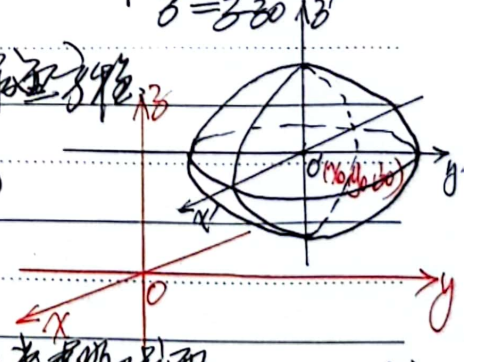
\includegraphics[width=0.3\textwidth]{figure/4-1.png}
    \caption{椭球面}
    \label{fig:椭球面}
\end{figure}

\subsubsection*{圆柱面}

$$
x^2 + y^2 = R^2
$$
为圆柱面,当$z$取任意值时,圆柱面无限延伸.或者说,圆柱面是由直线连续移动形成的,这类曲面称为直纹面.

若要表示$Oxy$平面中的圆$x^2 + y^2 = R^2$,
则应写为$\begin{cases}
    x^2 + y^2 = R^2\\
    z = 0
\end{cases}$,即圆柱面与$Oxy(z=0)$平面的交面.同理,$\begin{cases}
    x^2 + y^2 = R^2\\
    z = 2
\end{cases}$是空间中$z=2$平面上的圆.

\begin{figure}[htbp]
    \centering
    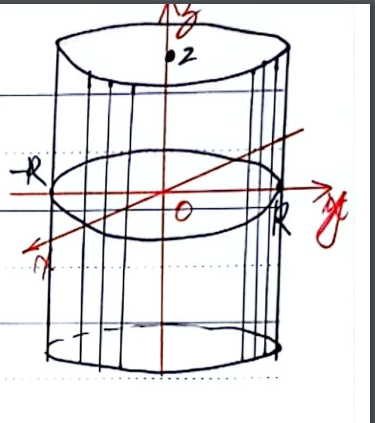
\includegraphics[width=0.3\textwidth]{figure/4-2.png}
    \caption{圆柱面}
    \label{fig:圆柱面}
\end{figure}

\subsubsection*{抛物柱面}

$
y^2 = 2px
$
及$y = a x^2( a , p \neq 0)$为抛物柱面.

$\begin{cases}
    y^2 = 2px\\
    z = 0
\end{cases},\begin{cases}
    y = ax^2\\
    z = 3
\end{cases}$为空间中的抛物线,这称为交面式的抛物线.

\begin{figure}[htbp]
    \centering
    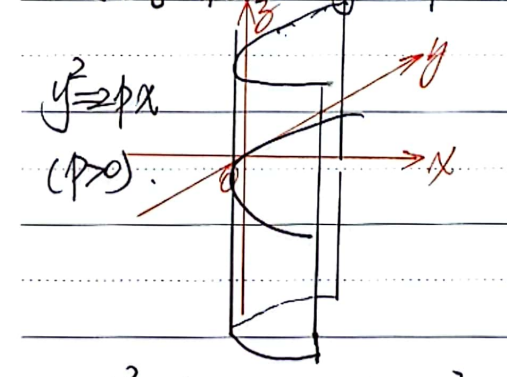
\includegraphics[width=0.3\textwidth]{figure/4-3.png}
    \caption{抛物柱面}
    \label{fig:抛物柱面}
\end{figure}

\subsubsection*{圆锥面}

$$
z^2 = a^2(x^2 + y^2)
$$

而$\begin{cases}
    z^2 = a^2(x^2 + y^2)\\
    z = c
\end{cases}$为空间中的圆;$\begin{cases}
    z = \pm ay\\
    x = 0
\end{cases}$为空间中的相交直线.

\begin{figure}[htbp]
    \centering
    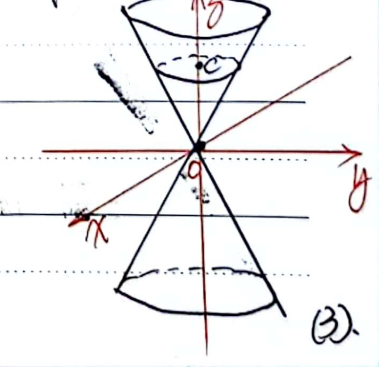
\includegraphics[width=0.3\textwidth]{figure/4-4.png}
    \caption{圆锥面}
    \label{fig:圆锥面}
\end{figure}

\subsubsection*{椭圆抛物面}

$$
z = \frac{x^2}{a^2} + \frac{y^2}{b^2},(a,b > 0)
$$

$\begin{cases}
    z = \frac{x^2}{a^2} + \frac{y^2}{b^2}\\
    z = z_0
\end{cases}$为空间中的椭圆,解$\frac{x^2}{a^2} + \frac{y^2}{b^2} = z_0$可得所围成的面积为$\pi(a\sqrt{z_0})(b\sqrt{z_0}) = \pi abz_0$.

\begin{figure}[htbp]
    \centering
    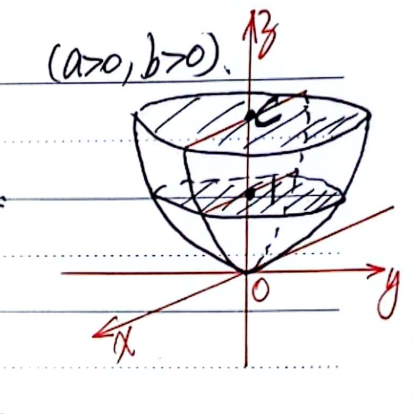
\includegraphics[width=0.3\textwidth]{figure/4-5.png}
    \caption{椭圆抛物面}
    \label{fig:椭圆抛物面}
\end{figure}


\subsubsection*{双曲抛物面}

$$
z = \frac{x^2}{a^2} - \frac{y^2}{b^2},(a,b > 0)
$$

又称为马鞍面.$z = z_0 > 0 $是一族实轴为$x$轴的双曲线,$z = z_0 < 0$是一族虚轴为$y$轴的双曲线.$\begin{cases}
    z = \frac{x^2}{a^2} - \frac{y^2}{b^2}\\
    x = 0
\end{cases}$是抛物线,$\begin{cases}
    z = \frac{x^2}{a^2} - \frac{y^2}{b^2}\\
    y = 0
\end{cases}$也是抛物线.故称双曲抛物面或马鞍面.易证,马鞍面是直纹面.

\begin{figure}[htbp]
    \centering
    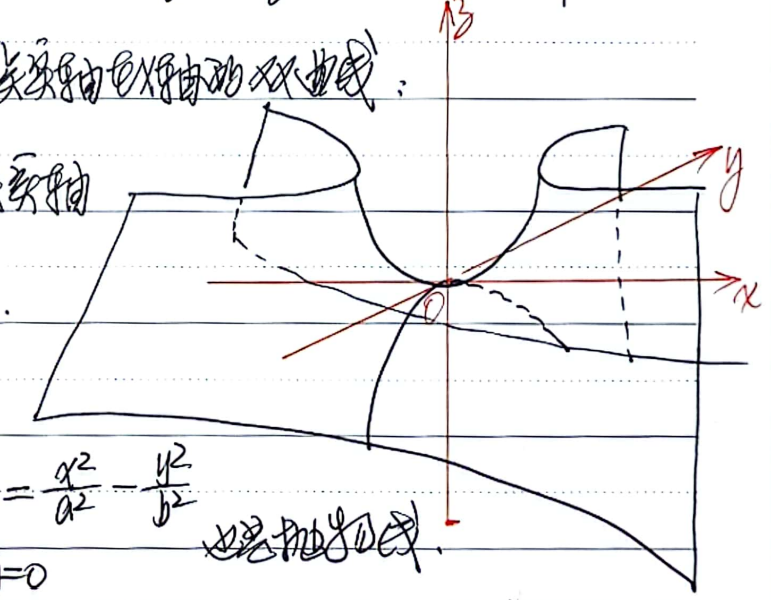
\includegraphics[width=0.3\textwidth]{figure/4-6.png}
    \caption{双曲抛物面}
    \label{fig:双曲抛物面}
\end{figure}

\subsubsection*{双叶双曲面}

$$
\frac{x^2}{a^2} + \frac{y^2}{b^2} - \frac{z^2}{c^2} = -1
$$

从$\frac{x^2}{a^2} + \frac{y^2}{b^2} = \frac{z^2}{c^2} - 1$可知$|z|\ges c$时,才有实点.当$z = z_0 > c$或$z = z_0 < -c$时,都是椭圆.


\begin{figure}[htbp]
    \centering
    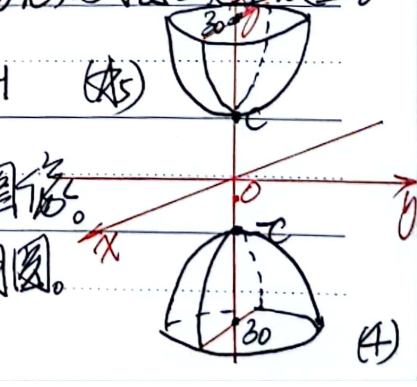
\includegraphics[width=0.3\textwidth]{figure/4-7.png}
    \caption{双叶双曲面}
    \label{fig:双叶双曲面}
\end{figure}

\subsubsection*{单叶双曲面}

$$
\frac{x^2}{a^2} + \frac{y^2}{b^2} - \frac{z^2}{c^2} = 1
$$

从$\frac{x^2}{a^2} + \frac{y^2}{b^2} = \frac{z^2}{c^2} + 1 \ges 0, \forall z$可知,对$z \in \R$,都有曲面图像,任取$z_0 \in \R$,$\begin{cases}
    \frac{x^2}{a^2} + \frac{y^2}{b^2} = \frac{z^2}{c^2} + 1\\
    z = z_0
\end{cases}$都是椭圆,即用垂直于$z$轴的平面去切单叶双曲面,截面都是椭圆.易证,单叶双曲面是由直线连续移动形成的直纹面.

\begin{figure}[htbp]
    \centering
    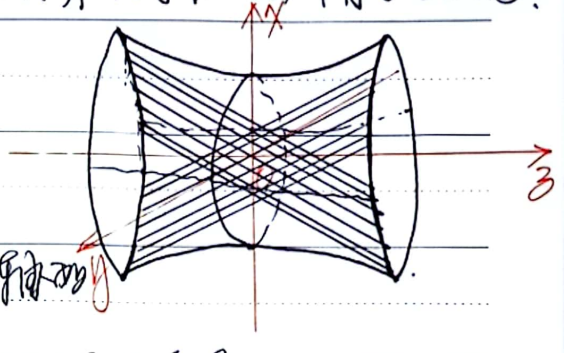
\includegraphics[width=0.3\textwidth]{figure/4-8.png}
    \caption{单叶双曲面}
    \label{fig:单叶双曲面}
\end{figure}

\section{旋转曲面}

设$L:z = f(y)$是一条平面曲线,将$L$绕$Ox$轴旋转一周,则所得曲面称为旋转曲面,记为$\Sigma$.设$M(x,y,z)$是$\Sigma$上一点,过点$M$作$Oz$轴的垂面交$Oz$轴于点$Q(0,0,z)$,交曲线$L$于点$A(0,y_1,z)$,则$| QM|^2 = | QA|^2 \Rightarrow x^2 + y^2 = y_1^2$,即$y_1 = \sqrt{x^2 + y^2}$,所以$\Sigma$的方程为$z = f(\pm \sqrt{x^2 + y^2})$.

\begin{figure}[htbp]
    \centering
    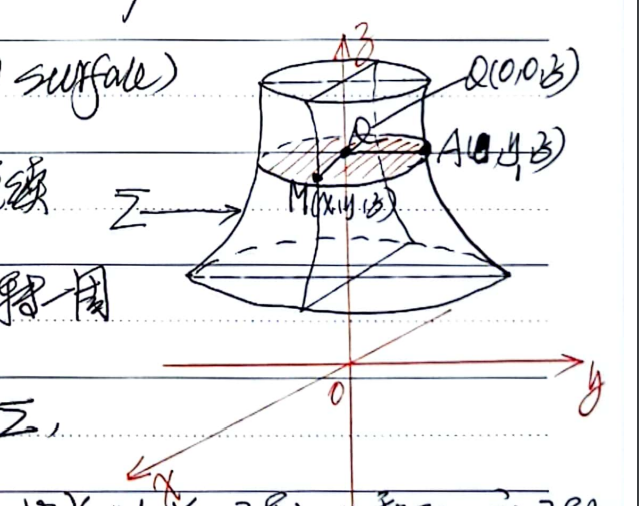
\includegraphics[width=0.3\textwidth]{figure/4-9.png}
    \caption{旋转曲面}
    \label{fig:旋转曲面}
\end{figure}

即曲线$z = f(y)$绕$Ox$轴旋转一周所得旋转曲面中$z$保持不变,而另一个变量用$\pm \sqrt{x^2 + y^2}$代替.同理,曲线$z = f(y)$绕$Oy$轴旋转一周所得旋转曲面中$z$保持不变,而另一个变量用$\pm \sqrt{x^2 + z^2}$代替.

\begin{example}
    证明:
    \begin{enumerate}
        \item 马鞍面:$z = \frac{x^2}{a^2} - \frac{y^2}{b^2}$是直纹面.
        \item 单叶双曲面:$\frac{x^2}{a^2} + \frac{y^2}{b^2} - \frac{z^2}{c^2} = 1$是直纹面.
    \end{enumerate}
\end{example}

\begin{proof}
    

    \begin{enumerate}
        \item 马鞍面可以化为$\left( \frac{x}{a} - \frac{y}{b} \right) \left( \frac{x}{a} + \frac{y}{b} \right) = z$,即$\begin{cases}
        \frac{x}{a} - \frac{y}{b} = \lambda\\
        \frac{x}{a} + \frac{y}{b} = \frac{z}{\lambda}
    \end{cases}$当$\lambda = 0$连续变化时,交面式的直线$L:\begin{cases}
        \frac{x}{a} - \frac{y}{b} = \lambda \\
        \frac{x}{a} + \frac{y}{b} = \frac{z}{\lambda}
    \end{cases}$连续变化,最后形成马鞍面.故马鞍面是直纹面.
        \item 从$\frac{x^2}{a^2} + \frac{y^2}{b^2} = \frac{z^2}{c^2} + 1$可知,对$\left( \frac{y}{b} - \frac{z}{c} \right) \left( \frac{y}{b} + \frac{z}{c} \right) = \left( 1 - \frac{x}{a} \right) \left( 1 + \frac{x}{a} \right)$,因此得到$\begin{cases}
        \frac{y}{b} - \frac{z}{c} = \lambda \left(1 - \frac{x}{a} \right)\\
        \frac{y}{b} + \frac{z}{c} = \frac{1}{\lambda} \left( 1 + \frac{x}{a} \right)
        \end{cases}$当$\lambda = 0$连续变化时,交面式的直线即单叶双曲面是由一族直线连续移动形成的,故单叶双曲面是直纹面.
    \end{enumerate}
\end{proof}


\begin{example}
    \textbf{球面三角形的余弦定理}

    设单位球面三角形$ABC$,是过球心$O$的三个平面$\pi_1,\pi_2,\pi_3$与球面$\Sigma: x^2 + y^2 + z^2 = 1$相交而成的球面上的三角形,如图所示:

    则有
    $$\cos a = \cos b \cos c + \sin b \sin c \cos A$$
    $$\cos b = \cos c \cos a + \sin c \sin a \cos B$$
    $$\cos c = \cos a \cos b + \sin a \sin b \cos C$$
\end{example}

\begin{figure}[htbp]
    \centering
    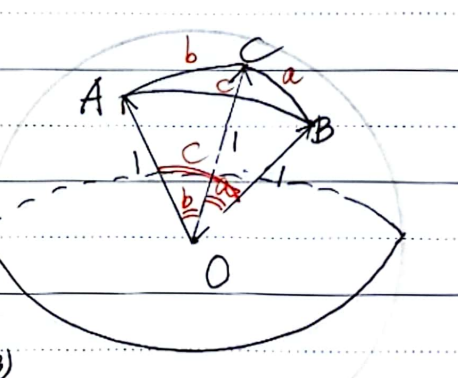
\includegraphics[width=0.5\textwidth]{figure/4-10.png}
    \caption{球面三角形}
    \label{fig:球面三角形}
\end{figure}

\begin{proof}
    $\overrightarrow{OB},\overrightarrow{OC}$确定了平面$\pi_1$,则法向量$\n_1 = \overrightarrow{OB} \times \overrightarrow{OC}$,同理可得$\n_2 = \overrightarrow{OC} \times \overrightarrow{OA},\n_3 = \overrightarrow{OA} \times \overrightarrow{OB}$.

    则
    $$ \cos A = \cos(\n_2,\n_3) = \frac{\n_2 \cdot \n_3}{| \n_2 | | \n_3 |} = \frac{(\overrightarrow{OC} \times \overrightarrow{OA}) \cdot (\overrightarrow{OA} \times \overrightarrow{OB})}{| \overrightarrow{OC} \times \overrightarrow{OA} | | \overrightarrow{OA} \times \overrightarrow{OB} |} $$

    依向量乘法以及Lagrange恒等式,及$| \overrightarrow{OA} \times \overrightarrow{OC} | = | \overrightarrow{OA} | | \overrightarrow{OC} | \sin(\overrightarrow{OA},\overrightarrow{OC}) = \sin b$,$| \overrightarrow{OA} \times \overrightarrow{OB} | = \sin c$,可得$(\overrightarrow{OA} \times \overrightarrow{OC}) \cdot (\overrightarrow{OA} \times \overrightarrow{OB}) = (\overrightarrow{OA} \cdot \overrightarrow{OA})(\overrightarrow{OC} \cdot \overrightarrow{OB}) - (\overrightarrow{OA} \cdot \overrightarrow{OB})(\overrightarrow{OC} \cdot \overrightarrow{OA}) = (| \overrightarrow{OA} |^2 \cos 0 ) (| \overrightarrow{OC}|| \overrightarrow{OB} | \cos a) - (| \overrightarrow{OA} | | \overrightarrow{OB} | \cos b)(| \overrightarrow{OC} | | \overrightarrow{OA} | \cos c) = \cos a - \cos b \cos c$.

    代入,得
    $$\cos A = \frac{\cos a - \cos b \cos c}{\sin b \sin c} \Rightarrow \cos a = \cos b \cos c + \sin b \sin c \cos A$$
    同理可得$\cos b = \cos c \cos a + \sin c \sin a \cos B,\cos c = \cos a \cos b + \sin a \sin b \cos C$.

\end{proof}

\begin{example}
    求曲线$L:\begin{cases}
        \frac{y^2}{a^2} + \frac{z^2}{b^2} = 1\\
        x = 0
    \end{cases}$绕$Oy$轴,$Oz$轴旋转一周所得曲面的方程.

\end{example}

\begin{solution}
\begin{enumerate}
    \item $L$绕$Oy$轴旋转一周,$y$保持不变,$z$用$\pm \sqrt{x^2 + z^2}$代替,则所得曲面方程为
    $\frac{y^2}{a^2} + \frac{x^2 + z^2}{b^2} = 1$,即$\frac{x^2}{b^2} + \frac{y^2}{a^2} + \frac{z^2}{b^2} = 1$.
    \item $L$绕$Oz$轴旋转一周,$z$保持不变,$y$用$\pm \sqrt{x^2 + y^2}$代替,则所得曲面方程为
    $\frac{x^2 + y^2}{a^2} + \frac{z^2}{b^2} = 1$,即$\frac{x^2}{a^2} + \frac{y^2}{a^2} + \frac{z^2}{b^2} = 1$.
\end{enumerate}
\end{solution}

\begin{example}
    求直线$L:\begin{cases}
        y = kx,k \neq 0\\
        z = 0
    \end{cases}$绕$Ox,Oy$轴旋转一周所得曲面的方程.
\end{example}

\begin{solution}
    \begin{enumerate}
        \item 绕$x$轴旋转时,$x$保持不变,$y$用$\pm \sqrt{y^2 + z^2}$代替,则所得曲面方程为
        $y = kx \Rightarrow kx = \pm \sqrt{y^2 + z^2}$,即$k^2x^2 = y^2 + z^2,k \neq 0$.
        \item 绕$y$轴旋转时,$y$保持不变,$x$用$\pm \sqrt{x^2 + z^2}$代替,则所得曲面方程为
        $y = kx \Rightarrow y = k \pm \sqrt{x^2 + z^2}$,即$y^2 = k^2(x^2 + z^2),k \neq 0$.
    \end{enumerate}

    两个旋转曲面都是圆锥面方程.
\end{solution}

\begin{figure}[htbp]
    \centering
    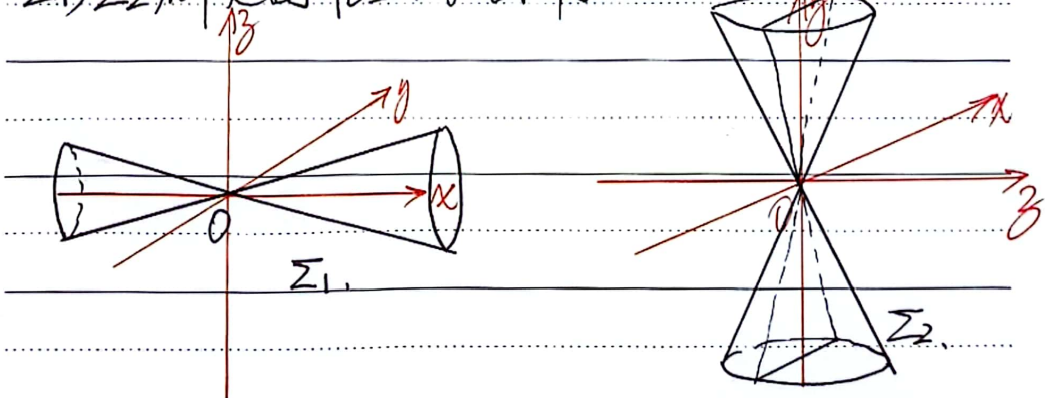
\includegraphics[width=0.8\textwidth]{figure/4-11.png}
    \caption{圆锥面}
    \label{fig:圆锥面}
\end{figure}


\begin{homework}
ex8.3:1,2,3.
\end{homework}








\setcounter{chapter}{4}
\chapter{空间解析几何综述}'

\section{坐标系的平移与旋转}

\begin{example}
    设有二次曲面$\Sigma:4x^2+25y^2+4z^2-16x-50y-16z-4z=0$,

    \begin{enumerate}
        \item 指出$\Sigma$是何种二次曲面;
        \item 将$\Sigma$一般化为参数式.
    \end{enumerate}
\end{example}\

\begin{solution}
\begin{enumerate}
    \item 配方得,$4(x-2)^2+25(y-1)^2+4(z-2)^2 = 100$,即
    $$
    \frac{(x-2)^2}{5^2}+\frac{(y-1)^2}{2^2}+\frac{(z-2)^2}{5^2} = 1
    $$
    故$\Sigma$是一个旋转椭球面.

    若令$\begin{cases}
        x-2 = x'\\
        y-1 = y'\\
        z-2 = z'
    \end{cases},M_0 = (2,1,2)=O'$,即是将坐标系的原点平移到$M_0$点,记作$O'$,新的经过平行移动得到的坐标系为$O'-x'y'z'$.
    在新坐标系下,$\Sigma$的方程为
    $$
    \frac{x'^2}{5^2}+\frac{y'^2}{2^2}+\frac{z'^2}{5^2} = 1
    $$
    \item 若令$\begin{cases}
        \frac{x'}{5} = \sin \theta \cos \varphi\\
        \frac{y'}{2} = \sin \theta \sin \varphi\\
        \frac{z'}{5} = \cos \theta
    \end{cases}$,则$\begin{cases}
        x' = 5\sin \theta \cos \varphi\\
        y' = 2\sin \theta \sin \varphi\\
        z' = 5\cos \theta
    \end{cases}, \theta \in [0,\pi],\varphi \in [0,2\pi]$
    即$\Sigma$的参数方程为
    $$
    \begin{cases}
        x = 2 + 5 \sin \theta \cos \varphi\\
        y = 1 + 2 \sin \theta \sin \varphi\\
        z = 2 + 5 \cos \theta
    \end{cases}, \theta \in [0,\pi],\varphi \in [0,2\pi]
    $$
    其中$\begin{cases}
        x' = 5\sin \theta \cos \varphi\\
        y' = 2\sin \theta \sin \varphi\\
        z' = 5\cos \theta
    \end{cases}, \theta \in [0,\pi],\varphi \in [0,2\pi]$是在新坐标系下的参数式,
    $\begin{cases}
        x = 2 + 5 \sin \theta \cos \varphi\\
        y = 1 + 2 \sin \theta \sin \varphi\\
        z = 2 + 5 \cos \theta
    \end{cases}, \theta \in [0,\pi],\varphi \in [0,2\pi]$是在原坐标系下的参数式.
\end{enumerate}
\end{solution}

\begin{remark}
    曲面$\Sigma$的参数式都是双参数的,但是参数式不是唯一的,例如
    $$
    \begin{cases}
        x = 2 + 5 \cos \theta \cos \varphi\\
        y = 1 + 2 \cos \theta \sin \varphi\\
        z = 2 + 5 \sin \theta
    \end{cases}, \theta \in [-\frac{\pi}{2},\frac{\pi}{2}],\varphi \in [0,2\pi]
    $$
    也是$\Sigma$的参数式.
\end{remark}

\begin{example}
    设有二次曲面$\Sigma:xy=z.$
    \begin{enumerate}
        \item 指出$\Sigma$是何种二次曲面;
        \item 求$\Sigma$的参数式.
    \end{enumerate}
\end{example}

\begin{solution}
    若保持坐标系的原点不动,让坐标系进行旋转变化.设$O-xyz$坐标系中,基向量为$\i,\j,\k$,在$O-x'y'z'$坐标系中,基向量为$\i',\j',\k'$,且$\i',\j',\k'$与$\i,\j,\k$的夹角如下表所示:
    \begin{table}[htbp]\label{ijk-i'j'k'}
        \centering
        \begin{tabular}{|c|c|c|c|}
            \hline
            & $\i$ & $\j$ & $\k$\\
            \hline
            $\i'$ & $\alpha_1$ & $\beta_1$ & $\gamma_1$\\
            \hline
            $\j'$ & $\alpha_2$ & $\beta_2$ & $\gamma_2$\\
            \hline
            $\k'$ & $\alpha_3$ & $\beta_3$ & $\gamma_3$\\
            \hline
        \end{tabular}
        \caption{}
    \end{table}

    \begin{figure}[htbp]
        \centering
        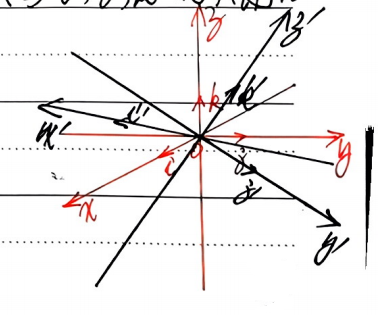
\includegraphics[width=0.3\textwidth]{figure/5-1.png}
        \caption{}
    \end{figure}

设$\overrightarrow{OM} = (a,b,c) \neq \theta$,则$\overrightarrow{OM}^\circ = \frac{\overrightarrow{OM}}{|\overrightarrow{OM}|} = (\frac{a}{|\overrightarrow{OM}|},\frac{b}{|\overrightarrow{OM}|},\frac{c}{|\overrightarrow{OM}|}) = (\cos \alpha, \cos \beta, \cos \gamma) = \cos \i + \cos \j + \cos \k$.
即单位向量$\overrightarrow{OM}^\circ$可以用他的三个方向余弦作为坐标,由表5.1得
$$
\begin{cases}
    \i' = \cos \alpha_1 \i + \cos \beta_1 \j + \cos \gamma_1 \k\\
    \j' = \cos \alpha_2 \i + \cos \beta_2 \j + \cos \gamma_2 \k\\
    \k' = \cos \alpha_3 \i + \cos \beta_3 \j + \cos \gamma_3 \k
\end{cases}
$$

现设点$Q$在$O-xyz$坐标系的坐标为$Q(x,y,z)$,在$O-x'y'z'$坐标系的坐标为$Q'(x',y',z')$,则
\begin{align*}
    \overrightarrow{OQ} &= x\i + y\j + z\k = x'\i' + y'\j' + z'\k'\\
    &= x'(\cos \alpha_1 \i + \cos \beta_1 \j + \cos \gamma_1 \k) + y'(\cos \alpha_2 \i + \cos \beta_2 \j + \cos \gamma_2 \k) + z'(\cos \alpha_3 \i + \cos \beta_3 \j + \cos \gamma_3 \k)\\
    &= (x' \cos \alpha_1 + y' \cos \alpha_2 + z' \cos \alpha_3)\i + (x' \cos \beta_1 + y' \cos \beta_2 + z' \cos \beta_3)\j + (x' \cos \gamma_1 + y' \cos \gamma_2 + z' \cos \gamma_3)\k
\end{align*}

也就是得到了
$$
\begin{cases}\label{X=AX'}
    x = x' \cos \alpha_1 + y' \cos \alpha_2 + z' \cos alpha_3\\
    y = x' \cos \beta_1 + y' \cos \beta_2 + z' \cos \beta_3\\
    z = x' \cos \gamma_1 + y' \cos \gamma_2 + z' \cos \gamma_3
\end{cases}
$$

若令$\X = \begin{pmatrix}
    x\\
    y\\
    z   
\end{pmatrix} , A = \begin{pmatrix}
    \cos \alpha_1 & \cos \alpha_2 & \cos \alpha_3\\
    \cos \beta_1 & \cos \beta_2 & \cos \beta_3\\
    \cos \gamma_1 & \cos \gamma_2 & \cos \gamma_3
\end{pmatrix} , \X' = \begin{pmatrix}
    x'\\
    y'\\
    z'
\end{pmatrix}$,则有$\X = A\X'$,即$\X' = A^{-1}\X$,其中$A$的各行各列都是单位向量,且任意两行(列)正交;
在线性代数中,称$A$这样的矩阵为正交矩阵,即$AA^T  = A^T A = I$,其中$I$是单位矩阵.
称$\ref{X=AX'}$为正交线性变化,简称正交变换.

不难验证,$A A^T = A^T A = I$,即便几何中的旋转或物理中刚体的旋转,在代数中对应正交变换.\ref{X=AX'}表明旋转之后,原坐标$x,y,z$与新坐标$x',y',z'$之间的对应关系是正交变换关系.

\begin{enumerate}
    \item 若保持$Oz$轴不便,让$Oxy$坐标平面绕$z$轴逆时针旋转$\frac{\pi}{4}$,得到了新坐标系$O-x'y'z'$,则有

\begin{table}[htbp]
    \centering
    \begin{tabular}{|c|c|c|c|}
        \hline
        & $\i$ & $\j$ & $\k$\\
        \hline
        $\i'$ & $\pi / 4$ & $\pi / 4$ & $\pi /2$\\
        \hline
        $\j'$ & $3\pi / 4$ & $\pi / 4$ & $\pi /2$\\
        \hline
        $\k'$ & $\pi / 2$ & $\pi / 2$ & $0$\\
        \hline
    \end{tabular}
\end{table}

即有
$$
\begin{cases}
    x = x' \cos \frac{\pi}{4} + y' \cos \frac{3\pi}{4} + z' \cos \frac{\pi}{2} = \frac{1}{\sqrt{2}}(x'-y')\\
    y = x' \cos \frac{\pi}{4} + y' \cos \frac{\pi}{4} + z' \cos \frac{\pi}{2} = \frac{1}{\sqrt{2}}(x'+y')\\
    z = x' \cos \frac{\pi}{2} + y' \cos \frac{\pi}{2} + z' \cos 0 = z'
\end{cases}
$$

利用此正交变换,可以将$\Sigma:xy=z$化为$\Sigma: \frac{1}{\sqrt{2}}(x'-y')\frac{1}{\sqrt{2}}(x'+y')=z'$,即$z' = \frac{x'^2}{2} - \frac{y'^2}{2}$,即$\Sigma$是一个双曲抛物面.
\item $\Sigma:xy = z$在原坐标系中的参数式为$\begin{cases}
    x = x+0y\\
    y = 0x+y\\
    z = xy
\end{cases}$,$x,y$为参数,则$\Sigma$在新坐标系中的参数式为:$\begin{cases}
    x' = x' +0y'\\
    y' = 0x'+y'\\
    z' = \frac{1}{2}(x'^2-y'^2)
\end{cases}$,$x',y'$为参数.

\end{enumerate}
\end{solution}

\section{柱面坐标系与球面坐标系}

\subsection{柱面坐标系}

$\R^3$空间中任一点$Q(x,y,z)$都可以看作是在半径为$r$的某个圆柱面:$x^2+y^2 = r^2$上.而圆柱面$x^2+y^2=r^2$上的点都可以用$r,\theta,z$这三个参数来确定,称$(r,\theta,z)$为点$Q$的柱面坐标.

\begin{figure}[htbp]
    \centering
    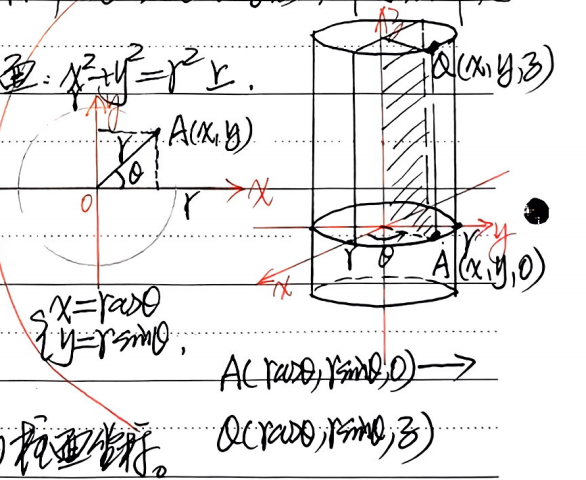
\includegraphics[width=0.3\textwidth]{figure/5-2.png}
    \caption{}
\end{figure}

\subsection{球面坐标系}

$\R^3$空间中任一点$Q(x,y,z)$都位于某个半径为$r$的球面$x^2+y^2+z^2=r^2$上,其中$r = | \overrightarrow{OQ} |$,$\overrightarrow{OQ}$与$Oz$轴的正向的夹角设为$\theta$,$\overrightarrow{OQ}$在$Oxy$平面中的投影与$Ox$轴正向夹角为$\varphi$,$0 \les \theta \les \pi, 0 \les \varphi \les 2 \pi$.
则$y = | \overrightarrow{OA}| \sin \varphi = r \sin \theta \sin \varphi$,而$z = r \cos \theta$.

称$(r,\theta,\varphi)$为点$Q$的球面坐标.球面坐标$r,\theta,\varphi$与直角坐标$x,y,z$之间的关系为
$$
\begin{cases}
    x = r \sin \theta \cos \varphi\\
    y = r \sin \theta \sin \varphi\\
    z = r \cos \theta
\end{cases},\theta \in [0,\pi],\varphi \in [0,2\pi], r \ges 0
$$

\begin{figure}[htbp]
    \centering
    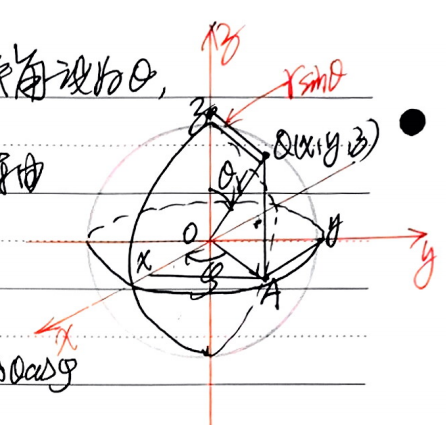
\includegraphics[width=0.3\textwidth]{figure/5-3.png}
    \caption{}
\end{figure}

直角坐标系下的球面方程:$\Sigma:x^2+y^2+z^2 = R^2$在柱面坐标系下$\begin{cases}
    x = r \cos \theta\\
    y = r \sin \theta\\
    z = z
\end{cases}$ 化为$\Sigma:r^2+z^2 = R^2$,即$\Sigma:r = R$.

在球面坐标系中,$\begin{cases}
    x = r \sin \theta \cos \varphi\\
    y = r \sin \theta \sin \varphi\\
    z = r \cos \theta
\end{cases}$下,化为$x^2+y^2+z^2 = r^2 = R^2$,即$\Sigma:r = R$.

双叶双曲面$\Sigma:x^2-y^2-z^2 = 1$在柱面坐标系中化为$r^2 \cos 2 \theta - z^2 = 1$,在球面坐标系中化为$2x^2 - (x^2 + y^2 + z^2) = 2(r \sin \theta \cos \varphi)^2 - r^2 = r^2 ( 2 \sin^2 \theta \cos^2 \varphi -1) = 1$.

\section{空间曲线的参数式}

空间曲线可以写为交线方程组$\begin{cases}
    F(x,y,z) = 0\\
    G(x,y,z) = 0
\end{cases}$,他可以改写为参数式.

\begin{example}
    将空间$\R^3$中的大圆周$\Gamma:\begin{cases}
        x^2+y^2+z^2 = a^2,a >0\\
        x+y+z = 0
    \end{cases}$化为参数式.
\end{example}

\begin{figure}[htbp]
    \centering
    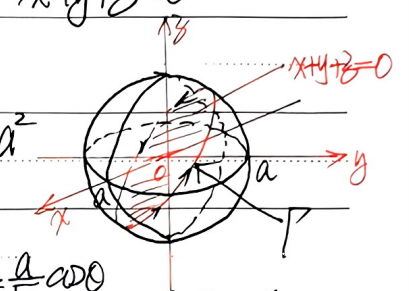
\includegraphics[width=0.3\textwidth]{figure/5-4.png}
    \caption{}
\end{figure}

\begin{solution}
    从$z = -(x+y) \Rightarrow x^2 + y^2 + (x+y)^2 = a^2 \Rightarrow x^2 +xy +y^2 = \frac{a^2}2 \Rightarrow \left( x+ \frac{y}{2} \right)^2 + \left( \frac{\sqrt{3}}{2}y \right)^2 = \left( \frac{a}{\sqrt{2}} \right)^2$.
    令$\begin{cases}
        x + \frac{y}{2} = \frac{a}{\sqrt{2}} \cos \theta\\
        \frac{\sqrt{3}}{2}y = \frac{a}{\sqrt{2}} \sin \theta
    \end{cases}, \theta \in [0,2\pi]$.则$y = \frac{2}{\sqrt{6}} a \sin \theta \Rightarrow x = \frac{a}{\sqrt{6}} (\sqrt3 \cos \theta - \sin \theta) \Rightarrow z = -(x+y) = \frac{-a}{\sqrt 6}(\sqrt 3 \cos \theta + \sin \theta)$.
    即圆周$\Gamma$的参数式为$\begin{cases}
        x = \frac{a}{\sqrt{6}} (\sqrt 3 \cos \theta - \sin \theta)\\
        y = \frac{2}{\sqrt{6}} a \sin \theta\\
        z = \frac{-a}{\sqrt{6}} (\sqrt 3 \cos \theta + \sin \theta)
    \end{cases}, \theta \in [0,2\pi]$.

\end{solution}


    若将$x$视为参数,则从$\begin{cases}
        F(x,y,z) = 0\\
        G(x,y,z) = 0
    \end{cases}$中可以解出$\begin{cases}
        x = x\\
        y = y(x)\\
        z = z(x)
    \end{cases},x \in I$.

\begin{example}
    空间中的直线$\Gamma:\begin{cases}
        x +y+z+5 =0\\
        x-y-2z -1=0
    \end{cases} \Leftrightarrow \begin{cases}
        y+3 = -x-5\\
        -y-2z = -x+1
    \end{cases} \Rightarrow \begin{cases}
        x = x\\
        y = -3x - 9\\
        z = 2x +4
    \end{cases}$.
\end{example}

\begin{remark}
    空间的曲线$\Gamma$的参数式中只有一个参数,且$\Gamma$的参数式不是唯一的.

\end{remark}

\begin{example}
    $\Gamma:\begin{cases}
        x = a \cos \theta\\
        y = a \sin \theta\\
        z = b \theta
    \end{cases},\theta \in [0,+\theta),a,b > 0$所表示的空间光滑曲线,称之为螺旋线.并称$k = 2\pi b$为一个螺距.

    \begin{figure}[htbp]
        \centering
        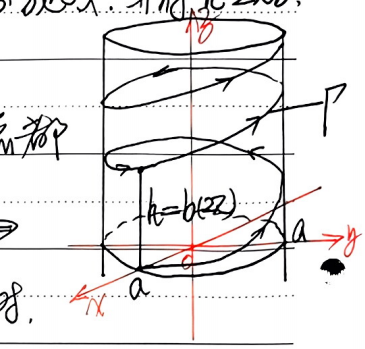
\includegraphics[width=0.3\textwidth]{figure/5-5.png}
        \caption{}
    \end{figure}

    此题中$x^2+y^2 \equiv a^2$,因此$\Gamma$上的点都在圆柱面$x^2+y^2 = a^2$上,而从$z = b \theta \Rightarrow z_\theta ' \equiv b$,即质点在作圆周运动的同时如果向上作匀速运动,
    则综合的结果是沿螺旋线作运动.

    无论是在物理中,还是在几何中,参数增加的方向被认为是曲线$\Gamma$的正向,相反的方向是曲线的负向.
\end{example}

\begin{homework}
ex8.4:1,2,4(4)(5)(6)(10),8,9,11.
\end{homework}























\setcounter{chapter}{5}
\chapter{多元函数的极限与连续性}

\section{多元函数的例子}

多元函数形如$u = f(x_1,x_2,\cdots,x_n)$,其中$x_1,x_2,\cdots,x_n$是自变量,$u$是因变量.

\begin{enumerate}
    \item $z = ax+by+c, (x,y) \in \R^2 = \{ (x,y) | x,y \in \R, x^2 + y^2 \les +\infty \}$: 平面方程;
    \item $z = \sqrt{R^2 - x^2-y^2}, (x,y) \in D: x^2 + y^2 \les R^2$: 上半球面;
    \item $f(x,y) = \left( \frac{1}{\sqrt{2\pi}} \right)^2 \e^{-\frac{x^2+y^2}{2}}$: 二元正态分布概率密度函数;
    \item $u = \ln(a^2 - x^2-y^2-z^2), x^2+y^2+z^2 < a^2, \Omega: x^2+y^2+z^2 < a^2$为开球体;
    \item $B(x,y) = \int_0^1 t^{x-1} (1-t)^{y-1} \dif t, x,y > 0$: 贝塔函数.
    \item $u = a_1 x_1 + a_2 x_2 + \cdots + a_n x_n$: $n$元线性函数.
    \item $Q(x_1,x_2,\cdots,x_n) = \sum_{i=1}^n \sum_{j=1}^n a_{ij} x_i x_j, a_{ij} = a_{ji}$: $x_1,x_2,\cdots,x_n$的二次齐次函数.
\end{enumerate}

多元函数中,最简单的是二元函数$z=f(x,y), (x,y) \in D.$ 且$z = f(x,y)$有直观图像 --- 空间的曲面.因此,二元函数是今后的重点讨论的多元函数.

\section{平面点集的若干概念}

二元函数$z = f(x,y)$的定义域$D$是平面$\R^2$的一个子集.

\begin{enumerate}
    \item 点$M_0$的$\delta$邻域$\overline U(M_0,\delta) := \{ M : |MM_0| = \rho(M,M_0) < delta \}$,
    即$\overline U(M_0,\delta) = \{ (x,y) | (x-x_0)^2 + (y-y_0)^2 < \delta^2 \} \subset D$.
    \item $D$的内点$M_0$ : $M_0 \in D$,且$\exists \delta > 0 $,使得$\overline U(M_0,\delta) \subset D$.
    \item $D$的外点$M_0$ : $M_0 \notin D$,且$\exists \delta > 0 $,使得$\overline U(M_0,\delta) \cap D = \varnothing$.
    \item $D$的边界点$M_0$ : $M_0$的任意$\delta$邻域中都同时含有$D$中点与$D^c$中点.点集$D$的边界点全体记作$\partial D: D$的边界.
    \item 由全体内点组成的点集称为开集,开集$D$的余集$D^c$称为闭集.闭集的余集是开集.
    \item 连通性:若$D$中任意两点$A,B$都可以用$D$中连续曲线连接,则称$D$是联通的.
    \item 开集若是联通的,称之为开区域,简称为区域,开区域$D$与$D$的边界$\partial D$之并,称之为闭区域,记作$\overline D = D \cup \partial D$.
    \begin{remark}
    讲义上此处写为$\overline{D} = D + \partial D$.两种写法是等价的.
\end{remark}
    \item 若$\exists R >0$,使得$D \subset \overline{U}(0,R)$,则称$D$是有界集.
\end{enumerate}

\begin{example}
    $\overline U(M_0,\delta), \R^2, x^2+y^2+z^2<a^2$都是开集,$\overline U(M_0,\delta)^c, x^2+y^2+z^2 < a^2$是有界集,$\R^2$是无界集.
    $(x-x_0)^2 + (y-y_0)^2 \ges \delta^2, (R^2)^c = \varnothing, x^2+y^2+z^2 \ges a^2$是闭集.
    $(x-x_0)^2 + (y-y_0)^2 \les \delta^2, x^2+y^2+z^2 \les a^2$是有界闭集.
\end{example}

\begin{example}
    空集$\varnothing$由零个内点组合,因此是开集;$\varnothing^c = \R^2$开,因此$\varnothing$是闭集.
    在所有点集之中,只有空集和全集是既开又闭的.
\end{example}

\section{二元函数$f(x,y)$的极限与连续性}

\begin{enumerate}
    \item 若$\forall \delta >0, \overline U(M_0,\delta)$都有点集$D$中点,则称$M_0$是$D$原点(极限点),$M_0$这个原点可以属于$D$,也可以不属于$D$.
    \item 设点$M_0 \in D$,且$\exists \delta > 0 $,使得$\overline U(M_0,\delta)$中除$M_0$无$D$中点,则称$M_0$是$D$的孤立点.
\end{enumerate}

\begin{definition}
    设 \( z = f(x, y) \) 是定义在平面点集 \( D \) 上的二维函数,\( M_0 = (x_0, y_0) \) 是 \( D \) 的聚点,又设 \( a \) 是一个数.如果对任意给定的 \( \epsilon > 0 \),存在 \( \delta > 0 \),当 \( M = (x, y) \in D \) 满足

$$
0 < \rho(M, M_0) = \sqrt{(x - x_0)^2 + (y - y_0)^2} < \delta
$$

或者
$$
0 < |x - x_0| < \delta, \quad 0 < |y - y_0| < \delta
$$

时,有
$$
|f(M) - a| < \varepsilon,
$$

那么称当 \( M \) 趋于 \( M_0 \) 时 \( f(M) \) 以 \( a \) 为极限,记作
$$
\lim_{M \to M_0} f(M) = a.
$$

也可以写成
$$
\lim_{(x, y) \to (x_0, y_0)} f(x, y) = a \quad \text{或} \quad \lim_{x \to x_0 , y \to y_0} f(x, y) = a.
$$
\end{definition}

由于多元函数的极限与一元函数的极限定义的方式相同.因此,一元函数极限中的四则运算法则,夹逼准则,及极限的唯一性,局部有界性,保号性,保序性等都可以推广到多元函数的极限之中来.

\begin{definition}
    设 \( f(x, y) \) 在 \( (x_0, y_0) \) 的邻域 \( B(M_0, r) = \{ M \mid \rho(M, M_0) < r \} \) 有定义, 如
$$
\rho = \sqrt{(x - x_0)^2 + (y - y_0)^2} < \delta,
$$

或者
$$
|x - x_0| < \delta, \quad |y - y_0| < \delta
$$

时, 就有
$$
|f(x, y) - f(x_0, y_0)| < \varepsilon
$$

也就是说极限
$$
\lim_{x \to x_0, y \to y_0} f(x, y) = f(x_0, y_0),
$$

或
$$
\lim_{\Delta x \to 0, \Delta y \to 0} f(x_0 + \Delta x, y_0 + \Delta y) = f(x_0, y_0),
$$

那么称 \( f \) 在 \( (x_0, y_0) \) 连续.如果 \( f \) 在区域 \( D \) 的每一个点连续,就称 \( f \) 在 \( D \) 上连续.
\end{definition}

\begin{remark}
    多元函数的一致连续性指的是$\delta$与$\varepsilon$与点$M_0$无关,具体而言,若$\forall \varepsilon > 0, \exists \delta > 0$,使得$\forall M_1,M_2 \in D$,当$\rho(M_1,M_2) < \delta$时,有$|f(M_1)-f(M_2)| < \varepsilon$,则称$f(x,y)$在$D$上一致连续.
\end{remark}

从定义可知,若$M_0$是$D$是原点,则必有$\lim_{M \to M_0} f(M) = f(M_0) = f(\lim_{M \to M_0} M)$,即极限号与函数符号可交换.

若$M_0(x_0,y_0)$是$D$的孤立点,则$f(M)$在$M_0$处必连续.

\begin{proof}
    $\forall \ve >0, \exists \delta >0$,使得$\overline U(M_0,\delta)$中除$M_0$外无$D$中点.当$M \in D, | MM_0 | < \delta $时,$|f(M) - f(M_0)| = 0 < \ve$,即$\lim_{M \to M_0} f(M) = f(M_0)$.
\end{proof}

\begin{remark}      
    此处使用的是课本上的定义方式.
\end{remark}

\begin{example}
    $f(x,y) = \sqrt{\cos^2 \pi x + \cos^2 \pi y -2}$的定义域$D$由所有的整点(格点)$M(m,n),m,n \in \Z$组成.每个整点都是$D$的孤立点.也都是$f(x,y)$的连续点,从而$f(x,y)$在$D$上连续.
\end{example}

\begin{example}
    考察下列极限:
    \begin{enumerate}
        \item 证明:$\lim_{x \to 0, y \to 0} \frac{x^2 y^2}{x^4 + y^2} =0$;
        \item 证明:$\lim_{x \to 0, y \to 0} \frac{x^2 y}{x^4 + y^2} $不存在;
        \item 证明:$\lim_{x \to 0, y \to 0} \left( 1 +xy \right)^{\frac{1}{x+y}} $不存在.
    \end{enumerate}
\end{example}

\begin{proof}
    \begin{enumerate}
        \item $0 \les \frac{x^2 y^2}{x^4 + y^2} \les \frac12 |y|$,且$\lim_{x \to 0, y \to 0} 0 = 0 = \lim_{x \to 0, y \to 0} \frac12 |y|$,由夹逼准则,得$\lim_{x \to 0, y \to 0} \frac{x^2 y^2}{x^4 + y^2} =0$;
        \item 取$y = kx^2$,$k$为常数,即动点$M(x,y)$沿抛物线$y = kx^2$趋于原点,则$\lim_{x \to 0, y \to 0} \frac{x^2 y}{x^4 + y^2} = \lim_{x \to 0} \frac{kx^3}{x^4 + k^2 x^4} = \lim_{x \to 0} \frac{k}{1+k^2} = \frac{k}{1+k^2}$.当$k$取不同值时,即动点以不同方式趋于$(0,0)$时,函数有不同的极限,与极限存在的唯一性矛盾.
        故$\lim_{x \to 0, y \to 0} \frac{x^2 y}{x^4 + y^2} $不存在,从而$\begin{cases}
            \frac{x^2 y}{x^4 + y^2} ,  x^2 + y^2 \neq 0\\
            0, x^2 + y^2 = 0
        \end{cases}$在$(0,0)$处不连续;
        \item $\lim_{x \to 0, y \to 0} \left( 1 +xy \right)^{\frac{1}{x+y}} = \lim_{x \to 0, y \to 0} \left( 1 +xy \right)^{\frac{1}{x+y} \cdot \frac{x+y}{xy}} $.其中
        $$
        \lim_{x \to 0, y \to 0} (1+xy)^{\frac{1}{xy}} = \lim_{u \to 0} (1+u)^{\frac{1}{u}} = \e
        $$ 

        而取$y = -x + kx^2$时,$\lim_{x \to 0, y \to 0} \frac{x+y}{xy} = \lim_{x \to 0, y \to 0} \frac{x+y}{xy} = \lim_{x \to 0, y \to 0} \frac{-x^2 + kx^3}{kx^2} = -\frac{1}{k}$.
        即$k$取不同值时,$M(x,y)$沿$y = -x + kx^2$趋于原点时,函数有不同的极限,与极限存在的唯一性矛盾.
        $\lim_{x \to 0 ,y \to 0} \frac{xy}{x+y} $不存在,从而$\lim_{x \to 0, y \to 0} \left( 1 +xy \right)^{\frac{1}{x+y}} $不存在.
    \end{enumerate}
\end{proof}

\begin{example}
    设$f(x,y) = \begin{cases}
        \frac{x^2 y}{x^4 + y^2}, x^2 + y^2 \neq 0\\
        0, x^2 + y^2 = 0
    \end{cases}$.证明在$(0,0)$处过此点的每一条射线$\begin{cases}
        x = t \cos \alpha \\
        y = t \sin \alpha
    \end{cases}, 0 \les t < + \infty$,$f(x,y)$都连续,即$\lim_{t \to \delta^+} f(t \cos \alpha, t \sin \alpha) = f(0,0) = 0$.但$f(x,y)$在$(0,0)$处不连续.
\end{example}

\begin{proof}
    不连续性已在上文证明.下证射线上的连续性.

    $\lim_{t \to 0^+} f(t \cos \alpha, t \sin \alpha) = \lim_{t \to 0^+} \frac{(t \cos \alpha)^2 (t \sin \alpha)}{(t \cos \alpha)^4 + (t \sin \alpha)^3} = \lim_{t \to 0^+} \frac{t \cos^2 \alpha \sin \alpha}{t^2 \cos^4 \alpha + \sin^2 \alpha} = 0 = f(0,0)$.
    因此对于任意$\alpha$,即对于任意射线,函数$f(x,y)$在射线上连续.
\end{proof}

\section{连续多元函数的主要性质}

\begin{enumerate}
    \item 连续多元函数的和,差,积,商(分母不为零)仍然是连续的多元函数;
    \item 在复合有意义的前提下,连续多元函数的复合函数仍是连续函数;
    \item 有界闭区域$D$上的连续多元函数具有“五性”;
    \begin{enumerate}
        \item 有界性;
        \item 最值性;
        \item 介值性;
        \item 零值性;
        \item 一致连续性,
    \end{enumerate}
\end{enumerate}

上述性质的证明方法,与一元连续函数的“五性”证明方法类似.

\begin{homework}
    ex9.1:12,13,14(2)(7)(9)(10),15,17(1),18.
\end{homework}
\setcounter{chapter}{6} % 设置章节计数器

\chapter{偏导数与全微分(total differential)}

\section{多元函数的偏导数(partial derivative)}

在多元函数$z=f(x,y),(x,y)\in D$中,设$M_0(x_0,y_0),M_1(x_0+\Delta x,y_0),M_2(x_0,y_0+\Delta y)\in D $,则
\begin{enumerate}
    \item $f(x_0+\Delta x,y_0)-f(x_0,y_0)$是固定$y$,仅让$x$发生变化而使得$z$产生的增量.
    \item $f(x_0,y_0+\Delta y)-f(x_0,y_0)$是固定$x$,仅让$y$发生变化而使得$z$产生的增量.
\end{enumerate}

记$\Delta z_x =f(x_0+\Delta x,y_0)-f(x_0,y_0),\Delta z_y =f(x_0,y_0+\Delta y)-f(x_0,y_0)$分别称作因变量$z$关于$x,y$的偏增量,并有如下定义:
\begin{definition}
    \begin{enumerate}
        \item $\lim_{\Delta x \to 0}\frac{f(x_0+\Delta x,y_0)-f(x_0,y_0)}{\Delta x}$为$z$关于$x$在$M_0(x_0,y_0)$处的偏导数,并记作
        $$\frac{\partial z}{\partial x}\bigg|_{M_0}=f'_x(M_0)=f'_x(x_0,y_0)=\lim_{\Delta x \to 0}\frac{f(x_0+\Delta x,y_0)-f(x_0,y_0)}{\Delta x}=\big(f(x,y_0)\big)'_x\bigg|_{x_0}$$

        \item $\lim_{\Delta y \to 0}\frac{f(x_0,y_0+\Delta y)-f(x_0,y_0)}{\Delta y}$为$z$关于$y$在$M_0(x_0,y_0)$处的偏导数,并记作
        $$\frac{\partial z}{\partial y}\bigg|_{M_0}=f'_y(M_0)=f'_y(x_0,y_0)=\lim_{\Delta y \to 0}\frac{f(x_0,y_0+\Delta y)-f(x_0,y_0)}{\Delta y}=\big(f(x_0,y)\big)'_y\bigg|_{y_0}$$
    \end{enumerate}
\end{definition}

\begin{remark}
    我们采用的几种导数记号:
    \begin{enumerate}
        \item $\frac{\partial z}{\partial x}\bigg|_{(x_0,y_0)}$;
        \item $\frac{\partial f}{\partial x}(x_0,y_0),\frac{\partial f(x_0,y_0)}{\partial x},\frac{\partial f}{\partial x}\bigg|_{(x_0,y_0)}$;
        \item $f'_x(x_0,y_0)$;
        \item $f'_1(x_0,y_0)$(一定程度上可以避免复合函数指代的问题,推荐使用).
    \end{enumerate}
\end{remark}

$f'_x(M_0),f'_y(M_0)$实际上就是在点$M_0$处,因变量$z$分别关于$x,y$的相对瞬时变化率.
即$$f'_x(x_0,y_0)=\frac{\dif{}f(x,y_0)}{\dif{}x}\bigg|_{x_0},f'_y(x_0,y_0)=\frac{\dif{}f(x_0,y)}{\dif{}y}\bigg|_{y_0}$$

同理,设$u=f(x,y,z)$在$\bar{U}(M_0,\Delta)$中有定义,则

$$f'_x(x_0,y_0,z_0)=\frac{\dif{}f(x,y_0,z_0)}{\dif{}x}\bigg|_{x_0},f'_y(x_0,y_0,z_0)=\frac{\dif{}f(x_0,y,z_0)}{\dif{}y}\bigg|_{y_0},f'_z(x_0,y_0,z_0)=\frac{\dif{}f(x_0,y_0,z)}{\dif{}z}\bigg|_{z_0}$$其余情形可类推.

总之,多元函数的偏导数,就是将多元函数中的其余自变量固定,只把因变量对一个自变量求导的结果.

\begin{example}
    设$f(x,y)=\begin{cases}
        \frac{x^2y}{x^4+y^2},&x^2+y^\neq0\\
        0,&x^2+y^2=0
    \end{cases}$
    \begin{enumerate}
        \item 证明$f(x,y)$在$(0,0)$处不连续;
        \item 证明$f'_x(0,0)=f'_y(0,0)=0$,即$f(x,y)$在$(0,0)$处可偏导;
        \item 求$f'_x(1,1),f'_y(2,1)$.
    \end{enumerate}
\end{example}
\begin{solution}
    \begin{enumerate}
        \item 沿着$y=kx^2$可得在$(0,0)$不连续.
        \item $f'_x(0,0)=\lim_{\Delta x\to 0}\frac{f(\Delta x,0)-f(0,0)}{\Delta x}=\lim_{\Delta x\to 0}\frac{\frac{(\Delta x)^2\cdot 0}{(\Delta x)^4+0^2}}{\Delta x}=\lim_{\Delta x\to 0}0=0$,同理$f'_y(0,0)=0$
        \item $f'_x(1,1)=\big(f(x,1)\big)'_x\bigg|_{x=1}=\left(\frac{x^2\cdot 1}{x^4+1^2}\right)'_x\bigg|_{x=1}=\frac{2x-2x^5}{(x^4+1)^2}\bigg|_{x=1}=0$
        
        $f'_y(2,1)=\big(f(2,y)\big)'_y\bigg|_{x=1}=\left(\frac{2^2y}{2^4+y^2}\right)'_y\bigg|_{y=1}=\frac{4(16-y^2)}{(16+y^2)^2}\bigg|_{y=1}=\frac{60}{289}$
    \end{enumerate}
\end{solution}

\begin{example}
    设$f(x,y)=\sqrt{x^2+y^2}$,证明:\begin{enumerate}
        \item $f(x,y)$在$(0,0)$处连续.
        \item $f(x,y)$在$(0,0)$处偏导数$f'_x(0,0),f'_y(0,0)$不存在,即$f(x,y)$在$(0,0)$处不可偏导.
    \end{enumerate}
\end{example}
\begin{proof}
    \begin{enumerate}
        \item $\lim_{\substack{x\to0\\y\to0}}\sqrt{x^2+y^2}=0=f(0,0)$
        \item $f'_x(0,0)=\big(\sqrt{x^2+0}\big)'_x\bigg|_{x=0}=\big(|x|\big)'_x\bigg|_{x=0}$不存在.同理$f'_y(0,0)$不存在.
    \end{enumerate}
\end{proof}
从两个例题可知,多元函数连续性和可偏导性没有关系.

\section{多元函数全微分(total differential)与可微性}
\begin{definition}
    设$z=f(x,y),(x,y)\in D\in \R^2$,并设$M_0(x_0,y_0),M(x_0+\Delta x,y_0+\Delta y)\in D $,若存在常数$A,B$,设$z=f(x,y)$在$M_0$处的全增量可表示为$$\Delta z=f(M)-f(M_0)=f(x_0+\Delta x ,y_0+\Delta y)-f(x_0,y_0)=A\Delta x+B\Delta y+o(\rho)$$q其中,$\rho=\rho(M,M_0)=\sqrt{(\Delta x)^2+(\Delta y)^2}$,则称$z=f(x,y)$是可微的.
    
    称$\Delta x,\Delta y$的线性函数:$A\Delta x+B\Delta y=A(x-x_0)+B(y-y_0)$为$f(x,y)$在$M_0$处的全微分,记作$\dif{}z\bigg|_{M_0}=A\Delta x+B\Delta y=A(x-x_0)+B(y-y_0)$

    即在$z=f(x,y)$在点$M_0(x_0,y_0)$可微的条件下,有$\Delta z=\dif{z}\bigg|_{M_0}+o(\rho)=A(x-x_0)+B(y-y_0)+o(\rho)$
\end{definition}

同理,若三元函数$u=f(x,y,z)$在点$M_0(x_0,y_0,z_0)$处的全增量可表示为
$$\Delta u=f(x_0+\Delta x,y_0+\Delta y,z_0+\Delta z)-f(x_0,y_0,z_0)+o(\rho)$$
其中$A,B,C$为常数,$\rho=\rho(M_0,M)=\sqrt{(\Delta x)^2+(\Delta y)^2+(\Delta z)^2}$,则称$u=f(x,y,z)$在点$M_0$处可微,且$A\Delta x+B\Delta y+C\Delta z$称为$f(x,y,z)$在点$M_0$处的全微分,记作$\dif{}u\bigg|_{M_0}=A\Delta x+B\Delta y+C\Delta z$
即有
$\Delta u=\dif{}u\bigg|_{M_0}+o(\rho)=A(x-x_0)+B(y-y_0)+C(z-z_0)+o(\rho)$
更高维上的可类似进行定义.

若$z=f(x,y)$在区域$D$中每一点可微,则称$f(x,y)$在区域$D$上可微.

\begin{remark}
    关于$\dif$这个符号,有如下几种认知,
    \begin{enumerate}
        \item 完全当做记号来用,即只有全微分,积分,以及有些情况下的导数才使用,实际上B2中也确实最好这么做.
        \item 如上述表述中的,作为线性主部存在,$\dif{}z=A(x-x_0)+B(y-y_0)$.但一般不用$\dif{}d z$去直接代替做运算.
        \item 特殊的线性映射,相当于认为$\dif{}z(\Delta x,\Delta y)\bigg|_{(x_0,y_0)}=A\Delta x+B\Delta y$,这是B3中的定义,了解一下即可.
        \item 一种特殊算子,在B2的后续选讲课程中微分形式涉及到这一部分,也是了解即可.
    \end{enumerate}
    我们在B2中实际上可以按照第二种方式去理解,但最好不要让$\dif{}z=A(x-x_0)+B(y-y_0)$这种形式出现,因为这种表达方式和另外三种都有些冲突,且容易出错.
    实际上更多的当成完全的记号来使用会更好.
\end{remark}

\begin{theorem}
    \begin{enumerate}
        \item 若$z=f(x,y)$在点$M_0(x_0,y_0)$处可微,则$f(x,y)$在$M_0$处连续.反之未必.
        \item 若$z=f(x,y)$在点$M_0(x_0,y_0)$处可微,则$f(x,y)$在$M_0$处可偏导.反之未必.
    \end{enumerate}
\end{theorem}
\begin{proof}
    \begin{enumerate}
        \item 
            \begin{enumerate}
                \item 当$\rho=\sqrt{(\Delta x)^2+(\Delta y)^2}\to 0$,有$\begin{cases}
                \Delta x\to 0,\\
                \Delta y\to 0;
                \end{cases}$而$$\lim_{\substack{\Delta x\to 0\\\Delta y \to 0}}\Delta z=\lim_{\substack{\Delta x\to 0\\\Delta y \to 0}}A\Delta x+B\Delta y+o(\rho)=0$$
                因此$$\lim_{\substack{\Delta x\to 0\\\Delta y \to 0}}f(x_0+\Delta x,y_0+\Delta y)=f(x_0,y_0)$$
                即有连续性.
                \item 反例:$z=\sqrt{x^2+y^2}$在原点处连续但不可微,否则原点处可偏导.
            \end{enumerate}
        \item 
            \begin{enumerate}
                \item $$\lim_{\Delta x\to 0}\frac{f(x_0+\Delta x,y_0)-f(x_0,y_0)}{\Delta x}=\lim_{\Delta x\to 0}\frac{A\Delta x+o(|\Delta x|)}{\Delta x}=A$$
                因此$f'_x(x_0,y_0)$存在,且$f'_x(x_0,y_0)=A$.
        
                同理,有$f'_x(x_0,y_0)$存在,$f'_y(x_0,y_0)=B$.故而可得偏导存在.
                \item 反例:$f(x,y)=\begin{cases}
                    \frac{x^2y}{x^4+y^2},&x^2+y^2>0\\
                    0,&x^2+y^2=0
                \end{cases}$在原点处可偏导但不连续,故一定不可微.
            \end{enumerate}
    \end{enumerate}
\end{proof}

\begin{example}
    证明:$f(x,y)=\begin{cases}
    \frac{x^2y}{x^2+y^2},&x^2+y^2>0\\
    0,&x^2+y^2=0
    \end{cases}$在原点处可偏导,连续,但不可微.
\end{example}
\begin{solution}
    \begin{enumerate}
        \item \begin{align*}
            0\les\left|\frac{x^2y}{x^2+y^2}\right|
            &=\frac{|x||y|\cdot |x|}{x^2+y^2}\\
            &\les\frac{\frac{1}{2}(x^2+y^2)\cdot |x|}{x^2+y^2}\\
            &=\frac{|x|}{2}\to 0
        \end{align*}
        故得连续.
        \item $$f'_x(0,0)=(\frac{x^2\cdot0}{x^4+0^2})'_x\bigg|_{x=0}=(0)'_x|_{x=0}=0$$
        $$f'_y(0,0)=(\frac{0^2\cdot y}{0^4+y^2})'_y\bigg|_{y=0}=(0)'_y\bigg|_{y=0}=0$$
        故得可偏导.
        \item 反证法:假设在原点处可微.则有$$f(\Delta x,\Delta y)-0=A\Delta x+B\Delta y+o(\rho)$$
        结合偏导数可知上述等式可化为
        $$\frac{(\Delta x)^2\Delta y}{(\Delta x)^2+(\Delta y)^2}=o(\rho)$$
        即$$\lim_{\rho \to 0}\frac{\frac{(\Delta x)^2\Delta y}{(\Delta x)^2+(\Delta y)^2}}{\sqrt{(\Delta x)^2+(\Delta y)^2}}=\lim_{\rho \to 0}\frac{(\Delta x)^2\Delta y}{((\Delta x)^2+(\Delta y)^2)^\frac{3}{2}}=0$$

        但当$$\lim_{\substack{\Delta x\to 0\\\Delta y=k\Delta x}}\frac{(\Delta x)^2\Delta y}{((\Delta x)^2+(\Delta y)^2)^\frac{3}{2}}=\lim_{\Delta x\to 0}\frac{(\Delta x)^2k\Delta x}{((\Delta x)^2+k(\Delta x)^2)^\frac{3}{2}}=\frac{k}{(1+k^2)^{\frac{3}{2}}}$$与$k$有关,故与极限存在唯一性矛盾,因此可知原函数在原点不可微.
    \end{enumerate}
\end{solution}

\begin{example}{思考题}
    设$u=f(x,y,z)=x^{y^z}+x^{a^z}+a^{y^z}+x^{y^a}+a^{a^z}(a>0,\text{常数})$
    求$\frac{\partial u}{\partial x},\frac{\partial u}{\partial y},\frac{\partial u}{\partial z}$,及$u$在$M(1,1,1)$处的全微分.
\end{example}
可不做在作业中,发在群里即可.

\begin{homework} 
    ex9.2:2(2)(5)(8),3,4,6,13(4)(6),16.
\end{homework}
\setcounter{chapter}{7}
\chapter{可微条件与高阶偏导数}

\section{$z = f(x,y)$在$M_0(x_0,y_0)$处可微的条件}

\begin{theorem}
    若$z = f(x,y)$在$M_0$处可微,则$f_x'(M_0),f_y'(M_0)$存在.反之未必.
\end{theorem}

\begin{proof}
    已知$z = f(x,y)$在$M_0(x_0,y_0)$处可微,则
    $$
    \Delta z = f(x_0 + \Delta x, y_0 + \Delta y) - f(x_0, y_0) = (A \Delta x + B \Delta y) + o(\rho),
    $$
    令$\Delta y = 0$,则
    $$
    \Delta z_x = f(x_0 + \Delta x, y_0) - f(x_0, y_0) = A \Delta x + o(|\Delta x|),
    $$
    由此得
    $$
    f_x'(M_0) = \lim_{\Delta x \to 0} \frac{f(x_0 + \Delta x, y_0) - f(x_0, y_0)}{\Delta x} = A.
    $$
    同理,令$\Delta x = 0$,则$f_y'(M_0) = B$.

    即$d z |_{M_0} = A \Delta x + B \Delta y = f_x'(M_0) \Delta x + f_y'(M_0) \Delta y \Rightarrow \dif z = f_x'(M_0) \Delta x + f_y'(M_0) \Delta y$.
    将$f_x'$记为$\frac{\partial f}{\partial x}$,将$f_y'$记为$\frac{\partial f}{\partial y}$,则
    $$
    \dif z = \frac{\partial f}{\partial x} \Delta x + \frac{\partial f}{\partial y} \Delta y = \frac{\partial f}{\partial x} \dif x + \frac{\partial f}{\partial y} \dif y.
    $$
    或者写成向量形式
    $$
    \dif z = \left( \frac{\partial f}{\partial x}, \frac{\partial f}{\partial y} \right) \begin{pmatrix}
        \dif x \\
        \dif y
    \end{pmatrix}.
    $$
\end{proof}

\begin{theorem}{thm:8.2}
    若$f(x,y)$在$M_0$处可微,则$z = f(x,y)$在$M_0$处必连续,反之未必.
\end{theorem}

\begin{proof}
    已知$\Delta z = f(x_0 + \Delta x, y_0 + \Delta y) - f(x_0, y_0) = f_x'(M_0) \Delta x + f_y'(M_0) \Delta y + o(\rho)$,且
    $$
    \Delta x \to 0, \Delta y \to 0,
    $$
    时,有
    $$
    f_x'(M_0) \Delta x + f_y'(M_0) \Delta y + o(\rho) \to 0, \quad o(\rho) \to 0,
    $$
    其中$\rho = \sqrt{(\Delta x)^2 + (\Delta y)^2}$,因此$\rho \to 0 \Leftrightarrow \Delta x \to 0, \Delta y \to 0$.

    从而$\lim_{\Delta x \to 0, \Delta y \to 0} \Delta z = 0 \Leftrightarrow z = f(x,y)$在$M_0$处连续.
\end{proof}

\begin{example}
    反例1: $z = f(x,y) = \sqrt{x^2 + y^2}$,在$M_0(0,0)$处连续.但因$f_x'(0,0) = f_y'(0,0) $都不存在,所以$f(x,y)$在$M_0$处不可微.
\end{example}

\begin{example}
    反例2: $z = f(x,y) = \begin{cases}
        \frac{x^2 y}{x^4 + y^2}, & (x,y) \neq (0,0), \\
        0, & (x,y) = (0,0).
    \end{cases}$
    在$(0,0)$处有$f_x'(0,0) = f_y'(0,0) = 0$,但$\lim_{(x,y) \to (0,0)} f(x,y)$不存在,所以$f(x,y)$在$(0,0)$处不连续.
    由\ref{thm:8.2}可知$f(x,y)$在$(0,0)$处不可微.
\end{example}

\begin{theorem}
    $z = f(x,y)$在$M_0(x_0,y_0)$处可微的充分必要条件是
    $$
    \lim_{\rho \to 0} \frac{\Delta z - f_x'(M_0)\Delta x - f_y'(M_0)\Delta y}{\rho} = 0.
    $$
\end{theorem}

\begin{proof}
    若$z = f(x,y)$在$M_0$处可微,则
    $$
    \Delta z = f(x_0 + \Delta x, y_0 + \Delta y) - f(x_0, y_0) = f_x'(M_0) \Delta x + f_y'(M_0) \Delta y + o(\rho),
    $$
    由此得
    $$
    \lim_{\rho \to 0} \frac{\Delta z - f_x'(M_0) \Delta x - f_y'(M_0) \Delta y}{\rho} = \lim_{\rho \to 0} \frac{o(\rho)}{\rho} = 0.
    $$

    反之,若
    $$
    \lim_{\rho \to 0} \frac{\Delta z - f_x'(M_0) \Delta x - f_y'(M_0) \Delta y}{\rho} = 0,
    $$
    则
    $$
    \Delta - (f_x'(M_0) \Delta x + f_y'(M_0) \Delta y) = o(\rho) \Rightarrow \Delta z = f_x'(M_0) \Delta x + f_y'(M_0) \Delta y + o(\rho) = (A \Delta x + B \Delta y) + o(\rho),
    $$
    从而$f(x,y)$在$M_0$处可微.
\end{proof}

\begin{theorem}
    $z = f(x,y)$在$M_0(x_0,y_0)$处可微的充分必要条件是$f_x'(x_0,y_0),f_y'(x_0,y_0)$存在且连续.
\end{theorem}

\begin{proof}
    已知$f_x'(x,y),f_y'(x,y)$在$M_0$处存在且连续,则
    \begin{align*}
        \Delta z &= f(x_0 + \Delta x, y_0 + \Delta y) - f(x_0, y_0) = \left[ f(x_0 + \Delta x, y_0 + \Delta y) - f(x_0, y_0 + \Delta y) \right] + \left[ f(x_0, y_0 + \Delta y) - f(x_0, y_0) \right] \\
        &= f_x'(x_0 + \theta_1 \Delta x, y_0 + \Delta y) \Delta x + f_y'(x_0, y_0 + \theta_2 \Delta y) \Delta y,
    \end{align*}
    其中$\theta_1, \theta_2 \in (0,1)$.利用$f_x'(x,y),f_y'(x,y)$的连续性,得
    $$
    \lim_{\Delta x \to 0, \Delta y \to 0} f_x'(x_0 + \theta_1 \Delta x, y_0 + \Delta y) = f_x'(x_0, y_0)
    $$
    $$
    \lim_{\Delta x \to 0, \Delta y \to 0} f_y'(x_0, y_0 + \theta_2 \Delta y) = f_y'(x_0, y_0),
    $$
    从而
    $$
    f_x'(x_0 + \theta_1 \Delta x, y_0 + \Delta y) = f_x'(x_0, y_0) + \alpha_1, \quad \alpha_1 \to 0, \ (\Delta x \to 0, \Delta y \to 0),
    $$
    $$
    f_y'(x_0, y_0 + \theta_2 \Delta y) = f_y'(x_0, y_0) + \alpha_2, \quad \alpha_2 \to 0, \ (\Delta x \to 0, \Delta y \to 0),
    $$
    即
    $$
    \Delta z = (f_x'(M_0) + \alpha_1) \Delta x + (f_y'(M_0) + \alpha_2) \Delta y = f_x'(M_0) \Delta x + f_y'(M_0) \Delta y + \alpha_1 \Delta x + \alpha_2 \Delta y,
    $$
    且$\lim_{\rho \to 0} \frac{\alpha_1 \Delta x + \alpha_2 \Delta y}{\rho} = \lim_{\rho \to 0} ( \alpha_1 \cos \theta + \alpha_2 \sin \theta) = 0$,从而$\alpha_1 \Delta x + \alpha_2 \Delta y = o(\rho)$,所以
    $$
    \Delta z = f_x'(M_0) \Delta x + f_y'(M_0) \Delta y + o(\rho) = (A \Delta x + B \Delta y) + o(\rho),
    $$
    从而$f(x,y)$在$M_0$处可微.
\end{proof}

\begin{example}
    反例3: $z = f(x,y) = \begin{cases}
        (x^2 +y^2) \sin \frac{1}{\sqrt{x^2 + y^2}}, & (x,y) \neq (0,0), \\
        0, & (x,y) = (0,0).
    \end{cases}$
    在$(0,0)$处可微,但$f_x'(x,y),f_y'(x,y)$在$(0,0)$处不连续.
\end{example}

\section{高阶偏导数}

设$z = f(x,y) = x^2 + xy+y^2 + x^y + 3x+4y$,则
\begin{align*}
    &\frac{\partial z}{\partial x} = 2x + y + y x^{y-1} + 3, \\
    &\frac{\partial z}{\partial y} = x + 2y + x^y \ln x + 4.
\end{align*}

由此得
\begin{align*}
    &\frac{\partial^2 z}{\partial y \partial x} = \left( \frac{\partial z}{\partial x} \right)_y' = (2x + y + yx^{y-1} +3)_y' = 1 + x^{y-1} + y x^{y-1} \ln x, \\
    &\frac{\partial^2 z}{\partial x \partial y} = \left( \frac{\partial z}{\partial y} \right)_x' = (x + 2y + x^y \ln x + 4)_x' = 1 + x^{y-1} + y x^{y-1} \ln x.
\end{align*}

进一步得
\begin{align*}
    &\frac{\partial^3 z}{\partial x \partial y \partial x} = \left( \frac{\partial^2 z}{\partial y \partial x} \right)_x' = \left( 1 + x^{y-1} + y x^{y-1} \ln x \right)_x' =(y-1) x^{y-2} + y(y-1)x^{y-2} \ln x + y x^{y-2},\\
    &\frac{\partial^3 z}{\partial x^2 \partial y} = \left( \frac{\partial^2 z}{\partial x \partial y} \right)_x' = \left( 1 + x^y \ln x + y \right)_x' = (y-1) x^{y-2} + y(y-1)x^{y-2} \ln x + y x^{y-2}.
\end{align*}

对比得知,$\frac{\partial^2 z}{\partial y \partial x} ,\frac{\partial^2 z}{\partial x \partial y},\frac{\partial^2 z}{\partial x \partial y \partial x},\frac{\partial^2 z}{\partial y \partial x \partial y}$在区域$D:x >0$ 中连续,且
\begin{align*}
    \frac{\partial^2 z}{\partial y \partial x} & \equiv \frac{\partial^2 z}{\partial x \partial y}, \\
    \frac{\partial^3 z}{\partial x \partial y \partial x} & \equiv \frac{\partial^3 z}{\partial x^2 \partial y}.
\end{align*}
对于$(x,y) \in D$成立.

\begin{theorem}
    若$z = f(x,y)$在区域$D$中的高阶偏导数连续,则高阶偏导数与求偏导的顺序无关.
\end{theorem}

\begin{proof}
    仅证$\frac{\partial^2 z}{\partial y \partial x} = \frac{\partial^2 z}{\partial x \partial y}$.
    
    任取$M_0 = (x_0,y_0) \in D, B(M_0, r) \subset D$,取$h = \Delta x \neq 0, k = \Delta y \neq 0$,使得$(x_0 + h, y_0 + k) \in B(M_0, r)$,令
    \begin{align*}
        \varphi(x) = f(x, y_0 + k) - f(x, y),\\
        \psi(y) = f(x_0 + h, y) - f(x_0, y).
    \end{align*}

    是$f(x, y)$分别对于$x$和$y$的偏差分。容易验证,如果$\varphi(x)$和$\psi(y)$分别对$x$和$y$再进行差分,那么差分的结果是都等于$f(x, y)$的二阶混合差分(下列第二个等式的右端)
\begin{align*}
    \varphi(x_0 +h) - \varphi(x_0) & = \psi(y_0 +k) - \psi(y_0) \\
    &= f(x_0 + h, y_0 + k) - f(x_0 + h, y_0) - f(x_0, y_0 + k) + f(x_0, y_0).
\end{align*}
由一元函数的微分公式可得
\begin{align*}
    \varphi(x_0 + h) - \varphi(x_0) & = h \varphi' (x_0 + \theta_1 h) \\
    & = h \left(f'(x_0 + \theta_1 h, y_0 + k) - f'(x_0 + \theta_1 h, y_0)\right) \\
    & = h k f''_{xy}(x_0 + \theta_1 h, y_0 + \eta_1 k),
\end{align*}
其中$0 < \theta_1, \eta_1 < 1$。类比存在$0 < \theta_2, \eta_2 < 1$,使得
$$
\psi(y + k) - \psi(y_0) = h k f''_{yx}(x_0 + \theta_2 h, y_0 + \eta_2 k).
$$
故有
$$
f''_{xy}(x_0 + \theta_1 h, y_0 + \eta_1 k) = f''_{yx}(x_0 + \theta_2 h, y_0 + \eta_2 k).
$$
令$(h, k) \to (0, 0)$,由混合偏导数的连续性即可证明定理。
\end{proof}

\section{例题}

\begin{example}
    证明函数$u = \frac{1}{r} , r = \sqrt{x^2 + y^2 + z^2 } >0$满足Laplace方程
    $$
    \frac{\partial^2 u}{\partial x^2} + \frac{\partial^2 u}{\partial y^2} + \frac{\partial^2 u}{\partial z^2} \equiv equiv 0, \forall (x,y,z) \neq (0,0,0).
    $$
\end{example}

\begin{proof}
    $u = (x^2 + y^2 + z^2)^{-\frac{1}{2}} \Rightarrow \frac{\partial u}{\partial x} = -x (x^2 + y^2 + z^2)^{-\frac{3}{2}} \Rightarrow \frac{\partial^2 u}{\partial x^2} = - \frac{(x^2+y^2+z^2)-3x^2}{(x^2+y^2+z^2)^{\frac{5}{2}}}$.
    由于$u = (x^2 + y^2 + z^2)^{-\frac{1}{2}}$是关于$x,y,z$的对称函数,因此有
    $$
    \frac{\partial^2 u}{\partial y^2} = - \frac{(x^2+y^2+z^2)-3y^2}{(x^2+y^2+z^2)^{\frac{5}{2}}}, \frac{\partial^2 u}{\partial z^2} = - \frac{(x^2+y^2+z^2)-3z^2}{(x^2+y^2+z^2)^{\frac{5}{2}}}.
    $$
    $$
    \frac{\partial^2 u}{\partial z^2} = - \frac{(x^2+y^2+z^2)-3z^2}{(x^2+y^2+z^2)^{\frac{5}{2}}}.
    $$
    从而
    $$
    \frac{\partial^2 u}{\partial x^2} + \frac{\partial^2 u}{\partial y^2} + \frac{\partial^2 u}{\partial z^2} = - \frac{3(x^2+y^2+z^2) - 3(x^2+y^2+z^2)}{(x^2+y^2+z^2)^{\frac{5}{2}}} = 0.
    $$
\end{proof}

\begin{example}
    证明$u = \frac{1}{2a \sqrt{\pi t}} \e^{ - \frac{x^2}{4a^2 t}}, x >0, t>0, a>0$常数满足热传导方程
    $$
    \frac{\partial u}{\partial t} = a^2 \frac{\partial^2 u}{\partial x^2}.
    $$
\end{example}

\begin{proof}
    \begin{align*}
        \frac{\partial u}{\partial t} & = \frac{(t^{-\frac12})_t'}{2a \sqrt \pi} \e^{-\frac{x^2}{4a^2 t}} + \frac{1}{2a \sqrt \pi} \e^{-\frac{x^2}{4a^2 t}} \left( - \frac{x^2}{4a^2t} \right)_t' \\
        &= \frac{1}{2a \sqrt{\pi t} t} \e^{-\frac{x^2}{4a^2 t}}\left( -1 + \frac{x^2}{2a^2 t} \right).
    \end{align*}
        且有
        \begin{align*}
            \frac{\partial u}{\partial x} & = \frac{1}{2a \sqrt{\pi t}} \e^{- \frac{x^2}{4a^2 t}} \left( - \frac{x}{2a^2 t} \right), \\
            \frac{\partial^2 u}{\partial x^2} & = \frac{1}{4a \sqrt{\pi t}t} \e^{- \frac{x^2}{4a^2 t}} \left( \frac{x^2}{2a^4 t} - \frac{1}{a^2} \right).
        \end{align*}
        从而
        $$
        a^2 \frac{\partial^2 u}{\partial x^2} = \frac{\partial u}{\partial t}, \quad \forall t >0, x \in \R^+.
        $$
\end{proof}

\begin{example}
    $\forall \phi,\psi \in C^2(I)$, $u = \phi(x - at) + \psi(x+ at)$满足波动方程
    $$
    \frac{\partial^2 u}{\partial t^2} = a^2 \frac{\partial^2 u}{\partial x^2}.
    $$
    其中$a >0$为常数.
\end{example}

\begin{proof}
    令$\begin{cases}
        v = x - at, \\
        w = x + at,
    \end{cases}$,则$u = \phi(v) + \psi(w)$,且
    \begin{align*}
        \frac{\partial u}{\partial x} & = \phi'(v) \frac{\partial v}{\partial x} + \psi'(w) \frac{\partial w}{\partial x} = \phi'(v) + \psi'(w), \\
        \frac{\partial u}{\partial t} & = \phi'(v) \frac{\partial v}{\partial t} + \psi'(w) \frac{\partial w}{\partial t} = -a \phi'(v) + a \psi'(w).
    \end{align*}
    从而
    \begin{align*}
        \frac{\partial^2 u}{\partial x^2} & = \phi''(v) \frac{\partial v}{\partial x} + \psi''(w) \frac{\partial w}{\partial x} = \phi''(v) + \psi''(w), \\
        \frac{\partial^2 u}{\partial t^2} & = \phi''(v) \frac{\partial v}{\partial t} + \psi''(w) \frac{\partial w}{\partial t} = a^2 \phi''(v) + a^2 \psi''(w).
    \end{align*}
    因此有
    $$
    \frac{\partial^2 u}{\partial t^2} = a^2 \frac{\partial^2 u}{\partial x^2}, \quad \forall t >0, x \in \R.
    $$
\end{proof}

\begin{homework}
ex9.2:2(7),8,11,15,26,27,28.
\end{homework}

\setcounter{chapter}{8} % 设置章节计数器

\chapter{复合(隐)函数微分法}

\section{复合函数(composition)微分法}

\begin{theorem}
    设$z=f(u,v)$在区域$D$中可微,且
    $\begin{cases}
        u=g(x,y)\\
        v=h(x,y)
    \end{cases}$都在区域$E$中可微,当复合$f(g(x,y),h(x,y))$有意义时,$z$通过中间变量$u,v$成为$x,y$的多元复合函数,且有求偏导数的链式法则如下:
    \begin{align}
        \begin{cases}
            \frac{\partial z}{\partial x}=\frac{\partial z}{\partial u}\frac{\partial u}{\partial x}+\frac{\partial z}{\partial v}\frac{\partial v}{\partial x},\\
            \frac{\partial z}{\partial y}=\frac{\partial z}{\partial u}\frac{\partial u}{\partial y}+\frac{\partial z}{\partial v}\frac{\partial v}{\partial y};\label{9.1}
        \end{cases}
    \end{align}

    同时,$z$作为$x,y$的多元复合函数可微,且不论$u,v$是作为$f(u,v)$的自变量,还是作为复合函数$f(g(x,y),h(x,y))$的中间变量,总有:
    \begin{align}
        \dif{}z=\frac{\partial z}{\partial u}\dif{}u+\frac{\partial z}{\partial v}\dif{}v.\label{9.2}
    \end{align}

    \ref{9.2}称为全微分的一阶形式不变性.
\end{theorem}

\begin{proof}
    \begin{enumerate}
        \item[\ref{9.1}] 固定$y$,令$x$有增量$\Delta x$,则
        $$\begin{cases}
            \Delta u_x = g(x+\Delta x,y)-g(x,y),\\
            \Delta v_x = h(x+\Delta x,y)-h(x,y),\\
            \Delta z_x = f(u+\Delta u_x,v+\Delta v_x)-f(u,v) = \frac{\partial z}{\partial u}\Delta u_x+\frac{\partial z}{\partial v}\Delta v_x + o(\rho);\\
        \end{cases}$$
        其中$\rho=\sqrt{\left(\Delta u_x\right)^2+\left(\Delta v_x\right)^2}$,并有$\Delta x\to 0\Rightarrow \begin{cases}
            \Delta u_x\to 0,\\
            \Delta v_x\to 0;
        \end{cases}\Rightarrow \rho \to 0.$

        利用
        \begin{align*}
            \lim_{\Delta x\to 0}\frac{o(\rho)}{\Delta x}
            &=\lim_{\Delta x\to 0}\frac{o(\rho)}{\rho}\frac{\rho}{\Delta x}\\
            &=\lim_{\Delta x\to 0}\frac{o(\rho)}{\rho}\lim_{\Delta x\to 0}\frac{\rho}{\Delta x}\\
            &=\lim_{\rho\to 0}\frac{o(\rho)}{\rho}\lim_{\Delta x\to 0}\sqrt{\left(\frac{\Delta u_x}{\Delta x}\right)^2+\left(\frac{\Delta v_x}{\Delta x}\right)^2}\\
            &=0\cdot\sqrt{\left(\frac{\partial u_x}{\partial x}\right)^2+\left(\frac{\partial v_x}{\partial x}\right)^2}\\&=0
        \end{align*}
        以及
            $$
            \lim_{\Delta x\to 0}\frac{\Delta u}{\Delta x}=\frac{\partial u}{\partial x},
            \lim_{\Delta x\to 0}\frac{\Delta v}{\Delta x}=\frac{\partial v}{\partial x};
            $$
        因此有
        \begin{align*}
            \frac{\partial z}{\partial x}
            &=\lim_{\Delta x\to 0}\frac{\Delta z_x}{\Delta x}\\
            &=\lim_{\Delta x\to 0}\left(\frac{\partial z}{\partial u}\frac{\Delta u_x}{\Delta x}+\frac{\partial z}{\partial v}\frac{\Delta v_x}{\Delta x}+ \frac{o(\rho)}{\Delta x}\right)\\
            &=\frac{\partial z}{\partial u}\lim_{\Delta x\to 0}\frac{\Delta u_x}{\Delta x}+\frac{\partial z}{\partial v}\lim_{\Delta x\to 0}\frac{\Delta v_x}{\Delta x}+ \lim_{\Delta x\to 0}\frac{o(\rho)}{\Delta x}\\
            &=\frac{\partial z}{\partial u}\frac{\partial u}{\partial x}+\frac{\partial z}{\partial v}\frac{\partial v}{\partial x}
        \end{align*}
        同理,对$y$有$$\frac{\partial z}{\partial y}=\frac{\partial z}{\partial u}\frac{\partial u}{\partial y}+\frac{\partial z}{\partial v}\frac{\partial v}{\partial y}$$
        \item[可微性] 
            记$$\begin{cases}
                \Delta u = g(x+\Delta x,y+\Delta y)-g(x,y),\\
                \Delta v = h(x+\Delta x,y+\Delta y)-h(x,y),\\
                \Delta z = f(u+\Delta u,v+\Delta v)-f(u,v),\\
                r = \sqrt{(\Delta x)^2+(\Delta y)^2},\\
                \rho =\sqrt{(\Delta u)^2+(\Delta v)^2};
                \end{cases}$$
            因此我们有
            \begin{align*}
                \Delta z
                &=\frac{\partial z}{\partial u}\Delta u+\frac{\partial z}{\partial v}\Delta v + o(\rho)\\
                &=\frac{\partial z}{\partial u} \left(\frac{\partial u}{\partial x}\Delta x+\frac{\partial u}{\partial y}\Delta y+o(r)\right) 
                + \frac{\partial z}{\partial v} \left(\frac{\partial v}{\partial x}\Delta x+\frac{\partial v}{\partial y}\Delta y+o(r)\right) + o(\rho)\\
                &=\left(\frac{\partial z}{\partial u}\frac{\partial u}{\partial x}+\frac{\partial z}{\partial v}\frac{\partial v}{\partial x}\right)\Delta x
                + \left(\frac{\partial z}{\partial u}\frac{\partial u}{\partial y}+\frac{\partial z}{\partial v}\frac{\partial v}{\partial y}\right)\Delta y + o(r) + o(\rho)\\
            \end{align*}
            同时,当$r\to 0$,有$\rho\to0$与$\frac{o(r)}{r}$有界,因此
            \begin{align*}
                \frac{\rho}{r}
                &=\frac{\sqrt{(\Delta u)^2+(\Delta v)^2}}{r}\\
                &=\sqrt
                {\left(\frac{\partial u}{\partial x}\frac{\Delta x}{r}+\frac{\partial u}{\partial y}\frac{\Delta y}{r}+\frac{o(r)}{r}\right)^2
                +\left(\frac{\partial v}{\partial x}\frac{\Delta x}{r}+\frac{\partial v}{\partial y}\frac{\Delta y}{r}+\frac{o(r)}{r}\right)^2}\\
                &\les \sqrt
                {\left(\frac{\partial u}{\partial x}\right)^2
                +\left(\frac{\partial u}{\partial y}\right)^2
                +\left(\frac{\partial v}{\partial x}\right)^2
                +\left(\frac{\partial v}{\partial y}\right)^2
                +M_0}\triangleq M,r\to0
            \end{align*}
            因此
            \begin{align*}
                \lim_{r\to 0}\left|\frac{o(\rho)}{r}\right|
                &=\lim_{r\to 0}\left|\frac{o(\rho)}{\rho}\right|\frac{\rho}{r}\\
                &\les M\lim_{r\to 0} \left|\frac{o(\rho)}{\rho}\right|\\
                &=0
            \end{align*}
            故$$\Delta z
            =\left(\frac{\partial z}{\partial u}\frac{\partial u}{\partial x}+\frac{\partial z}{\partial v}\frac{\partial v}{\partial x}\right)\Delta x
            +\left(\frac{\partial z}{\partial u}\frac{\partial u}{\partial y}+\frac{\partial z}{\partial v}\frac{\partial v}{\partial y}\right)\Delta y + o(r)$$
            表明$z$作为$x,y$的多元复合函数可微.
        \item[\ref{9.2}]
        \begin{enumerate}
            \item 当$u,v$作为$f(u,v)$的自变量时,$z=f(u,v)$可微,自然有$$\dif{}z=\frac{\partial z}{\partial u}\dif{}u+\frac{\partial z}{\partial v}\dif{}v.$$
            \item 当$u,v$作为复合函数$f(g(x,y),h(x,y))$的中间变量时,
            \begin{align*}
                \dif{}z
                &=\frac{\partial z}{\partial x}\dif{}x+\frac{\partial z}{\partial y}\dif{}y\\
                &=\left(\frac{\partial z}{\partial u}\frac{\partial u}{\partial x}+\frac{\partial z}{\partial v}\frac{\partial v}{\partial x}\right)\dif{}x
                +\left(\frac{\partial z}{\partial u}\frac{\partial u}{\partial y}+\frac{\partial z}{\partial v}\frac{\partial v}{\partial y}\right)\dif{}y\\
                &=\frac{\partial z}{\partial u} \left(\frac{\partial u}{\partial x}\dif{}x+\frac{\partial u}{\partial y}\dif{}y\right) 
                + \frac{\partial z}{\partial v} \left(\frac{\partial v}{\partial x}\dif{}x+\frac{\partial v}{\partial y}\dif{}y\right)\\
                &=\frac{\partial z}{\partial u}\dif{}u+\frac{\partial z}{\partial v}\dif{}v
            \end{align*}
        \end{enumerate}
    \end{enumerate}
\end{proof}

\section{隐函数(implicit function)微分法}
\begin{example}
    方程$$3x+4y-5z+7=0$$可确定$$
    \begin{cases}
        &z=\frac{3}{5}x+\frac{4}{5}y+\frac{7}{5},\\
        \text{or}& y=-\frac{3}{4}x+\frac{5}{4}z-\frac{7}{4},\\
        \text{or}& x=-\frac{4}{3}y+\frac{5}{3}z-\frac{7}{3};
    \end{cases}$$
    三个函数,分别可得
    $$
    \begin{cases}
        \frac{\partial z}{\partial x}=\frac{3}{5},\\
        \frac{\partial z}{\partial y}=\frac{4}{5};
    \end{cases}
    \begin{cases}
        \frac{\partial y}{\partial z}=\frac{5}{4},\\
        \frac{\partial y}{\partial x}=-\frac{3}{4};
    \end{cases}
    \begin{cases}
        \frac{\partial x}{\partial y}=-\frac{4}{3},\\
        \frac{\partial x}{\partial z}=\frac{5}{3};
    \end{cases}
    $$
    可得
    $$
    \frac{\partial z}{\partial x}\cdot\frac{\partial x}{\partial y}\cdot\frac{\partial y}{\partial z}=\frac{3}{5}\times\left(-\frac{4}{3}\right)\times\frac{5}{4}=-1,\\
    \frac{\partial x}{\partial z}\cdot\frac{\partial z}{\partial y}\cdot\frac{\partial y}{\partial x}=\frac{5}{3}\times\frac{4}{5}\times\left(-\frac{3}{4}\right)=-1.
    $$
    上述的三个二元函数,都是方程$F(x,y,z)=3x+4y-5z+7=0$所确定的隐函数.
\end{example}

\begin{theorem}
    设方程$F(x,y)=0$满足:
    \begin{enumerate}
        \item $F(x,y)\in C^1(D)$,$D$为区域,
        \item $F(M_0)=F(x_0,y_0)=0,M_0\in D,$
        \item $F'_y(M_0)=F'_y(x_0,y_0)\neq0.$
    \end{enumerate}
    则方程$F(x,y)=0$可在点$M_0$的某个$\delta$邻域$\bar{U}(M_0,\delta)$中确定唯一隐函数:$y=\varphi(x)$满足
    $$\begin{cases}
        \varphi(x_0)=y_0,\\
        \frac{\dif{}y}{\dif{}x}=\varphi'(x)=-\frac{F'_x(x,y)}{F'_y(x,y)}\in C
    \end{cases}$$
\end{theorem}
\begin{proof}
    不妨设$F'_y(x_0,y_0)>0$,则$F(x_0,y)$在$y_0$附近严格单调递增,即在$M(x_0,y_0)$附近形成了一条唯一存在的严格单调递增平面曲线,设此曲线的表达式为$y=\varphi(x),(x,y)\in \bar{U}(M_0,\delta)$,则$y=\varphi(x)$即为所求的隐函数.
    
    显然$y=\varphi(x)$穿过点$M_0(x_0,y_0)$,即$\varphi(x_0)=y_0$,且从$F(x,\varphi(x))\equiv 0$,两边对$x$求导,有:$F'_x\cdot 1+F'_y\cdot\frac{\dif{}\varphi(x)}{\dif{}x}\equiv 0\Rightarrow \frac{\dif{}y}{\dif{}x}=\varphi'(x)=-\frac{F'_x(x,y)}{F'_y(x,y)}$

    从$F\in C^1(D)$知,$\varphi'(x)$是连续函数.
\end{proof}

\begin{theorem}
    设方程$F(x,y,z)=0$满足:
    \begin{enumerate}
        \item $F(x,y,z)\in C^1(D)$,$D$为区域,
        \item $F(M_0)=F(x_0,y_0,z_0)=0,M_0\in D,$
        \item $F'_z(M_0)=F'_y(x_0,y_0,z_0)\neq0.$
    \end{enumerate}
    则方程$F(x,y,z)=0$可在点$M_0$的某个$\delta$邻域$\bar{U}(M_0,\delta)$中确定唯一隐函数:$z=\varphi(x,y)$满足
    $$\begin{cases}
        \varphi(x_0,y_0)=z_0,\\
        \frac{\partial z}{\partial x}=-\frac{F'_x(x,y,z)}{F'_z(x,y,z)},\frac{\partial z}{\partial y}=-\frac{F'_y(x,y,z)}{F'_z(x,y,z)}.
    \end{cases}$$
\end{theorem}

\begin{remark}
    值得注意的是,上述隐函数$y=\varphi(x)$或者$z=\varphi(x,y)$只理论上存在,实际问题中未必能求出来,但隐函数的导数或偏导数是能够从已知方程$F(x,y)=0$或$F(x,y,z)=0$中求出来的.

    例如,已知$z=\varphi(x,y)$是方程$F(x,y,z)=0$确定的隐函数,则由
    $F(x,y,\varphi(x,y))\equiv 0$,两边对$x,y$分别求导,有
    $$\begin{cases}
        F'_x\cdot 1+F'_z\cdot\varphi'_x(x,y)=0\\
        F'_y\cdot 1+F'_z\cdot\varphi'_y(x,y)=0
    \end{cases}\Rightarrow
    \begin{cases}
        \varphi'_x(x,y)=\frac{\partial z}{\partial x}=-\frac{F'_x(x,y,z)}{F'_z(x,y,z)}\\
        \varphi'_y(x,y)=\frac{\partial z}{\partial y}=-\frac{F'_y(x,y,z)}{F'_z(x,y,z)}.
    \end{cases}$$
\end{remark}

\section{例题}
\begin{example}
    证明:$$u=\frac{1}{r},r=\sqrt{x^2+y^2+z^2}$$满足Laplace方程:
    $$\frac{\partial^2u}{\partial x^2}+\frac{\partial^2u}{\partial y^2}+\frac{\partial^2u}{\partial z^2}\equiv 0,\forall (x,y,z)\neq(0,0,0).$$
\end{example}
\begin{proof}

    由于
    $\frac{\partial u}{\partial x}=\frac{\dif{}u}{\dif{}r}\frac{\partial r}{\partial x}=-\frac{1}{r^2}\frac{x}{r}=-\frac{x}{r^3},$

    因此$\frac{\partial^2 u}{\partial x^2}=-\left(\frac{x}{r^3}\right)'_x=-\frac{r^3-3r^2\frac{x}{r}x}{r^6}=-\frac{r^2-3x^2}{r^5},$

    由$u=\frac{1}{\sqrt{x^2+y^2+z^2}}$的对称性知$
    \begin{cases}
        \frac{\partial^2 u}{\partial y^2}=-\frac{r^2-3y^2}{r^5},\\
        \frac{\partial^2 u}{\partial z^2}=-\frac{r^2-3z^2}{r^5};
    \end{cases}$

    故$\frac{\partial^2u}{\partial x^2}+\frac{\partial^2u}{\partial y^2}+\frac{\partial^2u}{\partial z^2}=-\frac{3r^2-3(x^2+y^2+z^2)}{r^5}=-\frac{3r^2-3r^2}{r^5}=0.$
\end{proof}

\begin{example}
    证明:$$u=\frac{1}{2a\sqrt{\pi t}}\e^{-\frac{x^2}{4a^2t}}(x>0,t>0,a>0\text{常数})$$满足热传导方程:$$\frac{\partial u}{\partial t}=a^2\frac{\partial^2 u}{\partial x^2}.$$
\end{example}
\begin{proof}

    $\frac{\partial u}{\partial t}=\frac{1}{2a\sqrt{\pi}}(t^{-\frac{1}{22}})'_t \e^{-\frac{x^2}{4a^2t}}+\frac{1}{2a\sqrt{\pi t}}\e^{-\frac{x^2}{4a^2t}}(-\frac{x^2}{4a^2t})'_t=\frac{1}{4a\sqrt{\pi t^3}}\e^{-\frac{x^2}{4a^2t}}\left(\frac{x^2}{2a^2t}-1\right).$

    另外
    $\frac{\partial u}{\partial x}=\frac{1}{2a\sqrt{\pi t}}\e^{-\frac{x^2}{4a^2t}}\left(-\frac{x^2}{4a^2t}\right)'_x=\frac{1}{2a\sqrt{\pi t}}\e^{-\frac{x^2}{4a^2t}}\left(-\frac{x}{2a^2t}\right),$

    可得
    $\frac{\partial^2 u}{\partial x^2}=\frac{1}{2a\sqrt{\pi t}}\left[\e^{-\frac{x^2}{4a^2t}}\left(-\frac{x}{2a^2t}\right)^2+\e^{-\frac{x^2}{4a^2t}}\left(-\frac{1}{2a^2t}\right)\right]=\frac{1}{4a\sqrt{\pi t^3}}\e^{-\frac{x^2}{4a^2t}}\left(\frac{x^2}{2a^4t}-\frac{1}{a^2}\right),$

    因此$a^2\frac{\partial^2 u}{\partial x^2}=\frac{1}{4a\sqrt{\pi t^3}}\e^{-\frac{x^2}{4a^2t}}\left(\frac{x^2}{2a^2t}-1\right)=\frac{\partial u}{\partial t}.$
\end{proof}
 
\begin{example}
    证明:设$$\varphi,\psi\in C^2(I),u=\varphi(x-at)+\psi(x+at),(x\in\R,t>0,a>0\text{常数})$$满足波动方程:$$\frac{\partial^2 u}{\partial t^2}=a^2\frac{\partial^2 u}{\partial x^2}.$$
\end{example}
\begin{proof}

    令$\begin{cases}
        v=x-at,\\
        w=x+at;
    \end{cases}$则有$u=\varphi(v)+\psi(w)$且
    $\begin{cases}
        \frac{\partial v}{\partial x}=1,\\
        \frac{\partial w}{\partial x}=1;\\
    \end{cases}$与
    $\begin{cases}
        \frac{\partial v}{\partial t}=-a,\\
        \frac{\partial w}{\partial t}=a;\\
    \end{cases}$

    因此我们有$\frac{\partial u}{\partial x}=\varphi'(v)\frac{\partial v}{\partial x}+\psi'(w)\frac{\partial w}{\partial x}=\varphi'(v)+\psi'(w)$,
    
    故$\frac{\partial^ 2 u}{\partial x^2}=\varphi''(v)\frac{\partial v}{\partial x}+\psi''(w)\frac{\partial w}{\partial x}=\varphi''(v)+\psi''(w).$

    同时$\frac{\partial u}{\partial t}=\varphi'(v)\frac{\partial v}{\partial t}+\psi'(w)\frac{\partial w}{\partial t}=-a\varphi'(v)+a\psi'(w),$
    
    故$\frac{\partial^ 2 u}{\partial x^2}=-a\varphi''(v)\frac{\partial v}{\partial x}+a\psi''(w)\frac{\partial w}{\partial x}=a^2\left(\varphi''(v)+\psi''(w)\right)=a^2\frac{\partial^ 2 u}{\partial x^2}.$
\end{proof}

\begin{example}
    球面方程$x^2+y^2+z^2=a^2(a>0\text{常数})$在第一卦限内可确定三个隐函数
    $$x=\sqrt{a^2-y^2-z^2},y=\sqrt{a^2-x^2-z^2},z=\sqrt{a^2-x^2-y^2};
    $$
    证明:$$\frac{\partial x}{\partial y}\frac{\partial y}{\partial z}\frac{\partial z}{\partial x}\equiv -1.$$
\end{example}
\begin{proof}
    
    $\frac{\partial x}{\partial y}=-\frac{2y}{2\sqrt{a^2-y^2-z^2}}=-\frac{y}{x},$
    $\frac{\partial y}{\partial z}=-\frac{2z}{2\sqrt{a^2-x^2-z^2}}=-\frac{z}{y},$

    $\frac{\partial z}{\partial x}=-\frac{2x}{2\sqrt{a^2-x^2-y^2}}=-\frac{x}{z};$
    $(x>0,y>0,z>0),$
    
    因此$\frac{\partial x}{\partial y}\frac{\partial y}{\partial z}\frac{\partial z}{\partial x}=\left(-\frac{y}{x}\right)\left(-\frac{z}{y}\right)\left(-\frac{x}{z}\right)\equiv -1,\forall x>0,y>0,z>0,x^2+y^2+z^2=a^2.$
\end{proof}

\begin{example}
    设$F(x,y)\in C^2(D)$,$D$是区域,函数$y=\varphi(x)$由方程$F(x,y)=0$确定,
    
    证明:
    $$\varphi''(x)=\frac{\dif{}^2y}{\dif{}x^2}=-\frac{\frac{\partial^2F}{\partial x^2}\left(\frac{\partial F}{\partial y}\right)^2-2\frac{\partial^2F}{\partial x\partial y}\frac{\partial F}{\partial x}\frac{\partial F}{\partial y}+\frac{\partial^2F}{\partial y^2}\left(\frac{\partial F}{\partial x}\right)^2}{\left(\frac{\partial F}{\partial y}\right)^3}$$
\end{example}
\begin{proof}可知
    \begin{align*}
        \varphi''(x)
        &=\left(\varphi'(x)\right)'_x=-\left(\frac{F'_x(x,y)}{F'_y(x,y)}\right)'_x\\
        &=-\frac{\left(F'_x(x,y)\right)'_x F'_y(x,y)-\left(F'_y(x,y)\right)'_x F'_x(x,y)}{\left(F'_y(x,y)\right)^2}\\
        &=-\frac{\left(F''_{xx}\cdot1+F''_{xy}\cdot y'_x\right) F'_y-\left(F''_{yx}\cdot1+F''_{yy}\cdot y'_x\right) F'_x}{\left(F'_y\right)^2}\\
        &=-\frac{\left(F''_{xx}+F''_{xy}\left(-\frac{F'_x}{F'_y}\right)\right) F'_y-\left(F''_{yx}+F''_{yy}\left(-\frac{F'_x}{F'_y}\right)\right) F'_x}{\left(F'_y\right)^2}\\
        &=-\frac{F''_{xx}\left(F'_y\right)^2-F''_{xy}F'_x F'_y-F''_{xy}F'_x F'_y+F''_{yy}\left(F'_x\right)^2}{\left(F'_y\right)^3}\\
        &=-\frac{\frac{\partial^2F}{\partial x^2}\left(\frac{\partial F}{\partial y}\right)^2-2\frac{\partial^2F}{\partial x\partial y}\frac{\partial F}{\partial x}\frac{\partial F}{\partial y}+\frac{\partial^2F}{\partial y^2}\left(\frac{\partial F}{\partial x}\right)^2}{\left(\frac{\partial F}{\partial y}\right)^3}
    \end{align*}
    其中$y'_x=\frac{\dif{}y}{\dif{}x}=-\frac{F'_x(x,y)}{F'_y(x,y)}$.
\end{proof}
        
\begin{homework} 
    ex9.2:20(2)(3)(4),25,28,32;ex9.3:1(1),2(2)(5),4(1).
\end{homework}


\setcounter{chapter}{9} % 设置章节计数器

\chapter{多元函数微分法习题课(1)}

\section{例题}

\begin{example}
    设方程:$u^3 - 3(x+y) u^2 + z^3 = 0$确定了隐函数$u = f(x,y,z)$,求$\dif u$.
\end{example}

\begin{solution}
解法一:

原方程两边取全微分$\dif$,得
\begin{align*}
    & \diff (u^3 - 3(x+y) u^2 + z^3) = \diff (0) = 0 \\
    \Rightarrow &\diff(u^3) - 3 \diff((x+y)u^2) + \diff(z^3) = 0 \\
    \Rightarrow & 3u^2 \dif u - 3u^2 (\dif x + \dif y) - 3(x+y)2u \dif u + 3z^2 \dif z = 0 \\
\end{align*}

整理得
$$
\dif u = \frac{3u^2(\dif x + \dif y) + 3z^2 \dif z}{3u^2 + 6(x+y)u} = \frac{u^2 \dif x + u^2 \dif y - z^2 \dif z}{u^2 - 2(x+y)u}
$$
\end{solution}


\begin{solution}
解法二:

令$F(x,y,z,u) = u^3 - 3(x+y)u^2 + z^3 $,其中$x,y,z,u$地位相同,则$F_u' = 3u^2 - 6(x+y)u$,$F_x' = -3u^2$,$F_y' = -3u^2$,$F_z' = 3z^2$.从而
\begin{align*}
    \parfrac{u}{x} &= - \frac{F_x'}{F_u'} = \frac{u^2}{-2(x+y)u + u^2}; \\
    \parfrac{u}{y} &= - \frac{F_y'}{F_u'} = \frac{u^2}{-2(x+y)u + u^2}; \\
    \parfrac{u}{z} &= \frac{F_z'}{F_u'} = \frac{z^2}{-2(x+y)u + u^2}.
\end{align*}
因此
$$
\dif u = \parfrac{u}{x} \dif x + \parfrac{u}{y} \dif y + \parfrac{u}{z} \dif z = \frac{u^2 \dif x + u^2 \dif y - z^2 \dif z}{u^2 - 2(x+y)u}.
$$
\end{solution}

\begin{solution}
解法三:

原方程两边分别对$x,y,z$求偏导数,解出$\frac{\partial u}{\partial x},\frac{\partial u}{\partial y},\frac{\partial u}{\partial z}$再代入$\dif u = \frac{\partial u}{\partial x} \dif x + \frac{\partial u}{\partial y} \dif y + \frac{\partial u}{\partial z} \dif z$即可.
\end{solution}

\begin{example}
    试证明方程
    $$
    \parfrac{^2 u}{x^2} + 2 \parfrac{^2 u}{x,y} - 3 \parfrac{^2 u}{y^2} + 2 \parfrac{u}{x} + 6 \parfrac{u}{y} = 0
    $$
    在线性变换
    $$
    \begin{cases}
        \xi = x + y, \\
        \eta = 3x - y
    \end{cases}
    $$
    下可以化简为
    $$
    \parfrac{^2 u}{\xi,\eta} + \frac{1}{2} \parfrac{u}{\xi} = 0
    $$
\end{example}

\begin{solution}
    证法一:

    从线性变换$\begin{cases}
        \xi = x + y, \\
        \eta = 3x - y
    \end{cases}$可得$x = \frac{1}{4}(\xi + \eta)$,$y = \frac{1}{4}(3\xi - \eta)$,因此$\parfrac{x}{\xi} = \frac14,\parfrac{x}{\eta} = \frac14,\parfrac{y}{\xi} = \frac34,\parfrac{y}{\eta} = -\frac14$.由此得
    \begin{align*}
        \parfrac{u}{\xi} &= \parfrac{u}{x} \parfrac{x}{\xi} + \parfrac{u}{y} \parfrac{y}{\xi} = \frac14 \parfrac{u}{x} + \frac34 \parfrac{u}{y} \\
        \Rightarrow \parfrac{^2 u}{\eta,\xi} &= \left( \parfrac{u}{\xi} \right)'_{\eta} = \left( \frac14 \parfrac{u}{x} \right)_\eta' + \left( \frac34 \parfrac{u}{y} \right)_\eta'\\
        &= \frac14 \left( \parfrac{^2 u}{x^2} \parfrac{x}{\eta} + \parfrac{^2 u}{x,y} \parfrac{y}{\eta} \right) + \frac34 \left( \parfrac{^2 u}{x,y} \parfrac{x}{\eta} + \parfrac{^2 u}{y^2} \parfrac{y}{\eta} \right)\\
        &= \frac14 \left( \parfrac{^2 u}{x^2} \frac14 + \parfrac{^2 u}{x,y} \left( -\frac14 \right) \right) + \frac34 \left( \parfrac{^2 u}{x,y} \frac14 + \parfrac{^2 u}{y^2} \left( -\frac14 \right) \right)\\
        &= \frac{1}{16} \left( \parfrac{^2 u}{x^2} + 2 \parfrac{^2 u}{x,y} - 3 \parfrac{^2 u}{y^2} \right)
    \end{align*}

    即有$$
    \begin{cases}
        &\parfrac{^2 u}{x^2} + 2 \parfrac{^2 u}{x,y} - 3 \parfrac{^2 u}{y^2} = 16 \parfrac{^2 u}{\eta,\xi} \\
        & \parfrac{u}{x} + 3 \parfrac{u}{y} = 4 \parfrac{u}{\xi}
    \end{cases}$$

    故原偏微分方程化简为
    \begin{align*}
        &16 \parfrac{^2 u}{\eta,\xi} + 2 \left( 4 \parfrac{u}{\xi} \right) = 0 \\
        \Rightarrow &\parfrac{^2 u}{\eta,\xi} + \frac12 \parfrac{u}{\xi} = 0
    \end{align*}
\end{solution}

\begin{solution}
    解法二:

    从线性变换$\begin{cases}
        \xi = x + y, \\
        \eta = 3x - y
    \end{cases} \Rightarrow \parfrac{\xi}{x} = 1, \parfrac{\xi}{y} = 1, \parfrac{\eta}{x} = 3, \parfrac{\eta}{y} = -1$.而$u(x,y)$通过中间变量可视为$\xi,\eta$的函数,从而
    $$
    \begin{cases}
        \parfrac{u}{x} = \parfrac{u}{\xi} \parfrac{\xi}{x} + \parfrac{u}{\eta} \parfrac{\eta}{x} = \parfrac{u}{\xi} + 3 \parfrac{u}{\eta}, \\
        \parfrac{u}{y} = \parfrac{u}{\xi} \parfrac{\xi}{y} + \parfrac{u}{\eta} \parfrac{\eta}{y} = \parfrac{u}{\xi} - \parfrac{u}{\eta}.
    \end{cases},
    $$
    从而
    $$
    \begin{cases}
        \parfrac{^2 u}{x^2} = \left( \parfrac{u}{\xi} \right)_x' + 3 \left( \parfrac{u}{\eta} \right)_x' = \left( \parfrac{^2 u}{\xi^2} + 3 \parfrac{^2 u}{\eta,\xi}  \right) + 3 \left( \parfrac{^2 u}{\xi,\eta} +3 \parfrac{^2 u}{\eta^2} \right), \\
        \parfrac{^2 u}{x,y} = \left( \parfrac{u}{\xi} - \parfrac{u}{\eta} \right)_x' = \left( \parfrac{^2 u}{\xi^2} + 3 \parfrac{^2 u}{\xi,\eta} \right) - \left( \parfrac{^2 u}{\xi,\eta} +3 \parfrac{^2 u}{\eta^2} \right), \\
        \parfrac{^2 u}{y^2} = \left( \parfrac{u}{\xi} - \parfrac{u}{\eta} \right)_y' = \left( \parfrac{^2 u}{\xi^2} - \parfrac{^2 u}{\xi,\eta} \right) - \left( \parfrac{^2 u}{\xi,\eta} - \parfrac{^2 u}{\eta^2} \right).
    \end{cases}
    $$
    即
    $$
    \begin{cases}
        \parfrac{^2 u}{x^2} = \parfrac{^2 u}{\xi^2} + 6 \parfrac{^2 u}{\xi,\eta} + 9 \parfrac{^2 u}{\eta^2}, \\
        \parfrac{^2 u}{x,y} = \parfrac{^2 u}{\xi^2} + 2 \parfrac{^2 u}{\xi,\eta} - 3 \parfrac{^2 u}{\eta^2}, \\
        \parfrac{^2 u}{y^2} = \parfrac{^2 u}{\xi^2} - 2 \parfrac{^2 u}{\xi,\eta} + \parfrac{^2 u}{\eta^2}.
    \end{cases}
    $$
    且
    $$ 2 \parfrac{u}{x} + 6 \parfrac{u}{y} = 2 \left( \parfrac{u}{\xi} + 3 \parfrac{u}{\eta} \right) + 6 \left( \parfrac{u}{\xi} - \parfrac{u}{\eta} \right) = 8 \parfrac{u}{\xi},
    $$
    从而原方程化为
    $$
    \parfrac{^2 u}{\xi^2} (1+2-3) + \parfrac{^2 u}{\xi,\eta} (6+4+6) + \parfrac{^2 u}{\eta^2} (9-6-3) + 8 \parfrac{u}{\xi} = 0,
    $$
    即
    $$
    \parfrac{^2 u}{\xi,\eta} + \frac12 \parfrac{u}{\xi} = 0.
    $$
\end{solution}

\begin{example}
    设$u = f(x,y,z), \varphi(x^2,\e^y,z)=0, y = \sin x$,且$f,\varphi \in C^1, \parfrac{\varphi}{z} \neq 0$,求$\frac{\dif u}{\dif x}$.
\end{example}

\begin{solution}
    从$\varphi(x^2, \e^{\sin x},z) = 0$及$\varphi_z' \neq 0$可知,由方程$\varphi(x^2, \e^{\sin x},z) = 0$可确定$z $ 是$x,y$的隐函数,从而$z$是$x$的复合函数.故从$u = f(x,y,z)$知,$u$是$x$的一元函数.

    \begin{remark}
        助教注:这个地方可以理解为由隐函数定理$F(x,y,z) = \varphi(x^2, \e^y, z)=0$,确定了隐函数$z = z(x,y)$,从而$u =f(x,y,z) = f(x,y,z(x,y))=f(x,\sin x, z(x,\sin x))$确定了$u$是$x$的函数.
    \end{remark}
    $$
    \frac{\dif u}{\dif x} = f_1' \cdot 1 + f_2' \cdot y_x' + f_3' \cdot z_x' = f_1' + f_2' \cdot \cos x \cdot 2x + f_3' \cdot z_x'.
    $$
    令$F(x,y,z) = \varphi(x^2, \e^y, z)$,则
    $$
    \begin{cases}
        F_x'(x,y,z) = \varphi_1' \cdot 2x + \varphi_2' \e^{\sin x} \cos x,\\
        F_z'(x,y,z) = \varphi_3' \cdot 1 = \varphi_3'.
    \end{cases}
    $$
    故
    $z_x' = - \frac{F_x'}{F_z'} = - \frac{\varphi_1' \cdot 2x + \varphi_2' \e^{\sin x} \cos x}{\varphi_3'}$.代入$\frac{\dif u}{\dif x}$即有
    $$
    \frac{\dif u}{\dif x} = f_1' + f_2' \cdot y_x' + f_3' \cdot \left( - \frac{\varphi_1' \cdot 2x + \varphi_2' \e^{\sin x} \cos x}{\varphi_3'} \right).
    $$

    \begin{remark}
        助教注: 这里老师写的确实很模糊.我们要区分两个式子和他们分别的含义.
        \begin{enumerate}
            \item 令$F(x,y,z) = \varphi(x^2, \e^y, z)$,则$F(x,y,z) = 0$确定了$z = z(x,y)$,其中$z_x' = - \frac{F_x'}{F_z'}$.这时候$z_x'$表示的是$\parfrac{z}{x}$.
            $F_x'(x,y,z) = \varphi_1' \cdot 2x, F_z'(x,y,z) = \varphi_3'$,从而$z_x' = - \frac{F_x'}{F_z'} = - \frac{2x \varphi_1'}{\varphi_3'}$.
            \item 令$F(x,z) = \varphi(x^2, \e^{\sin x}, z)$,则$F(x,z) = 0$确定了$z = z(x)$.这时候$z_x'$表示的是$\frac{\dif z}{\dif x}$.
            $F_x'(x,z) = \varphi_1' \cdot 2x + \varphi_2' \e^{\sin x} \cos x, F_z'(x,z) = \varphi_3'$,从而$z_x' = - \frac{F_x'}{F_z'} = - \frac{2x \varphi_1' + \varphi_2' \e^{\sin x} \cos x}{\varphi_3'}$.
        \end{enumerate}
        老师要表示的实际是第二种情况,即$z = z(x)$.只不过写成的形式看起来像是第一种情况.
    \end{remark}
    \begin{remark}
        正是因为老师这里写模糊了,所以会有疑问为什么当$F(x,z) = \varphi(x^2, \e^{\sin x}, z)$时, $$F_x' = \varphi_1' \cdot 2x + \varphi_2' \e^{\sin x} \cos x$$而不是$$F_x' = \varphi_1' \cdot 2x + \varphi_2' \cdot \e^{\sin x} \cos x+\varphi_3' \cdot z_x'$$
        后者是$F(x) = \varphi(x^2, \e^{\sin x}, z(x))$时的$F_x' = F'(x)$.而为了求$\frac{\dif z}{\dif x}$,我们需要对$F(x,z)$这个函数利用隐函数定理,此时$x,z$都是这个$F(x,z)$的自变量,因此$F_x'=\varphi_1' \cdot 2x + \varphi_2' \e^{\sin x} \cos x$.
    \end{remark}
\end{solution}

\begin{example}
    证明:全微分也具有一阶微分形式不变性,即,若$f(x,y)$可微,则不论$x,y$是自变量还是中间变量,则$z = f(x,y)$,总有
    $$ \dif z= \dif f(x,y) = \parfrac{z}{x} \dif x + \parfrac{z}{y} \dif y = f_x' \dif x + f_y' \dif y. $$
\end{example}

\begin{proof}
    \begin{enumerate}
        \item 当$x,y$是自变量时,显然有$\dif z = f_x' \dif x + f_y' \dif y$.
        \item 当$x,y$是中间变量时,设$\begin{cases}
            x = g(s,t),\\
            y = h(s,t),
        \end{cases}$可微,且$f(g(s,t),h(s,t))$有意义时,$z$通过中间变量$x,y$成为$s,t$的复合函数,且有求偏导数的链式法则如下:
        \begin{align*}
            &\dif x = \parfrac{x}{s} \dif s + \parfrac{x}{t} \dif t,\\
            &\dif y = \parfrac{y}{s} \dif s + \parfrac{y}{t} \dif t.
        \end{align*}
        且
        \begin{align*}
            \dif z&= \parfrac{z}{s} \dif s + \parfrac{z}{t} \dif t = \left( \parfrac{z}{x} \cdot \parfrac{x}{s} + \parfrac{z}{y} \cdot \parfrac{y}{s} \right) \dif s + \left( \parfrac{z}{x} \cdot \parfrac{x}{t} + \parfrac{z}{y} \cdot \parfrac{y}{t} \right) \dif t \\
            &=\parfrac{z}{x} \left(\parfrac{x}{s} \dif s + \parfrac{x}{t} \dif t \right) + \parfrac{z}{y} \left( \parfrac{y}{s} \dif s + \parfrac{y}{t} \dif t \right)\\
            &= \parfrac{z}{x} \dif x+ \parfrac{z}{y} \dif y.
        \end{align*}
        即$x,y$是中间变量时,也有$\dif z = f_x' \dif x + f_y' \dif y$.
    \end{enumerate}
\end{proof}

\begin{remark}
    利用全微分的一阶微分形式不变性,可导出多元可微函数的如下的微分四则运算法则:
    \begin{enumerate}
        \item $\diff ( u \pm v) = \dif u \pm \dif v$;
        \item $\diff (uv) = u \dif v + v \dif u$;
        \item $\diff \left( \frac{u}{v} \right) = \frac{v \dif u - u \dif v}{v^2}$,其中$u,v$均可微,且$v \neq 0$;
    \end{enumerate}
\end{remark}

\begin{proof}
    \begin{enumerate}
        \item 令$f(u,v) = u+v$,则$f(u,v) \in C^1$,从而$f(u,v)$可微,无论$u,v$是自变量还是中间变量,总有
    $$
    \diff( u + v) = \dif f(u,v) = \parfrac{f}{u} \dif u + \parfrac{f}{v} \dif v = \dif u +\dif v
    $$
    从而有$\diff(u \pm v) = \dif u \pm \dif v$.这里$d$是全微分.
    \item 令$f(u,v) = uv$,则$f(u,v) \in C^1$,从而$f(u,v)$可微,无论$u,v$是自变量还是中间变量,总有
    $$
    \diff(uv) = \dif f(u,v) = \parfrac{f}{u} \dif u + \parfrac{f}{v} \dif v = v \dif u + u \dif v
    $$
    从而有$\diff(uv) = u \dif v + v \dif u$.
    \item 令$f(u,v) = \frac{u}{v}$,则$f(u,v) \in C^1$,从而$f(u,v)$可微,无论$u,v$是自变量还是中间变量,总有
    $$
    \diff \left( \frac{u}{v} \right) = \dif f(u,v) = \parfrac{f}{u} \dif u + \parfrac{f}{v} \dif v = \frac{1}{v} \dif u + \left( -\frac{u}{v^2} \right) \dif v = \frac{v \dif u - u \dif v}{v^2}
    $$
    \end{enumerate}
    
\end{proof}

\begin{remark}
    二阶及以上的微分通常没有形式不变性,具体而言,设$f(x,y) \in C^2$,则$z = f(x,y) \Rightarrow \dif z= \parfrac{z}{x} \dif x + \parfrac{z}{y} \dif y$.
    \begin{align*}
        \diff(\dif z) &:= \dif{^2} z = \diff \left( \parfrac{z}{x} \dif x+ \parfrac{z}{y} \dif y \right)\\
        &= \left( \parfrac{z}{x} \dif x+ \parfrac{z}{y} \dif y \right)_x' \dif x + \left( \parfrac{z}{x} \dif x + \parfrac{z}{y} \dif y \right)_y' \dif y\\
        &= \left( \parfrac{^2 z}{x^2} \dif x + \parfrac{^2 z}{x,y} \dif y \right) \dif x + \left( \parfrac{^2 z}{x,y} \dif x + \parfrac{^2 z}{y^2} \dif y \right) \dif y\\
        &= \parfrac{^2 z}{x^2} (\dif x)^2 + 2 \parfrac{^2 z}{x,y} \dif x \dif y + \parfrac{^2 z}{y^2} (\dif y)^2.
    \end{align*}
    $\dif{^2} z$是$x,y$是自变量时的$z = f(x,y)$的二阶微分,而$\dif{^2} z$是$x,y$是中间变量时的$z = f(x,y)$的二阶微分,二者通常不相等.
\end{remark}

\begin{example}
    设$u = u(x,y) , v=v(x,y)$是由方程组
    $$
    \begin{cases}
        u = f(ux,v+y),\\
        v = g(u-x,v^2y)
    \end{cases}
    $$所确定的隐函数组,求变换$\begin{cases}
        u = u(x,y),\\
        v = v(x,y)
    \end{cases}$的Jacobi行列式:
    $$
    \begin{vmatrix}
        u_x' & u_y'\\
        v_x' & v_y'
    \end{vmatrix} := \frac{\partial(u,v)}{\partial(x,y)}  \quad f,g \in C^1.
    $$
\end{example}

\begin{solution}
    令$A = ux, B = v+y,E = u-x, F = v^2y$,则方程组可化为
    $$
    \begin{cases}
        u = f(A,B),\\
        v = g(E,F).
    \end{cases}
    $$
    方程组两边关于$x$求偏导
    $$\begin{cases}
        u_x' = f_1' \cdot ( u + x u_x' ) + f_2' \cdot (v_x' + 0),\\
        v_x' = g_1' \cdot (u_x' - 1) + g_2' \cdot 2v v_x' y.
    \end{cases}$$
    标准化为
    $$
    \begin{cases}
        (x f_1' -1) u_x' + f_2' v_x' = -f_1' u,\\
        g_1' u_x' + (2v g_2' y - 1) v_x' = g_1'.
    \end{cases}
    $$
    令$D = \begin{vmatrix}
        x f_1' - 1 & f_2'\\
        g_1' & 2v g_2' y - 1
    \end{vmatrix}$,则$D \neq 0$,再令
    $$
    D_1 = \begin{vmatrix}
        -f_1' u & f_2'\\
        g_1' & 2v g_2' y - 1
    \end{vmatrix}, \quad D_2 = \begin{vmatrix}
        x f_1' - 1 & -f_1' u\\
        g_1' & g_1'
    \end{vmatrix},
    $$
    由克莱姆法则可得
    $$
    u_x' = \frac{D_1}{D}, \quad v_x' = \frac{D_2}{D}.
    $$
    方程组$\begin{cases}
        u = f(A,B),\\
        v = g(E,F)
    \end{cases}$两边同时对$y$求偏导,可得
    $$
    \begin{cases}
        u_y' = f_1' \cdot u_y' \cdot x + f_2' \cdot (v_y'+1),\\
        v_y' = g_1' \cdot u_y' + g_2' \cdot (2 v v_y' y + 2v^2).
    \end{cases}
    $$
    标准化为
    $$
    \begin{cases}
        (x f_1' - 1) u_y' + f_2' v_y' = -f_2',\\
        g_1' u_y' + (2v g_2' y - 1) v_y' = 2v g_2'.
    \end{cases}
    $$
    令$D = \begin{vmatrix}
        x f_1' - 1 & f_2'\\
        g_1' & 2v g_2' y - 1
    \end{vmatrix}$,则$D \neq 0$,再令
    $$
    \tilde{D_1} = \begin{vmatrix}
        -f_2' & f_2'\\
        v^2 g_2' & 2v g_2' y - 1
    \end{vmatrix}, \quad \tilde{D_2} = \begin{vmatrix}
        x f_1' - 1 & -f_2'\\
        g_1' & g_1'v^2
    \end{vmatrix},
    $$
    由克莱姆法则可得
    $$
    u_y' = \frac{\tilde{D_1}}{D}, \quad v_y' = \frac{\tilde{D_2}}{D}.
    $$
    从而
    $$
    \frac{\partial(u,v)}{\partial(x,y)}
    = \begin{vmatrix}
        u_x' & u_y'\\
        v_x' & v_y'
    \end{vmatrix} = \frac{\begin{vmatrix}
        D_1 & \tilde{D_1}\\
        D_2 & \tilde{D_2}
    \end{vmatrix}}{D}
    $$
\end{solution}

\begin{example}
    设$\begin{cases}
        u = u(x,y),\\
        v = v(x,y)
    \end{cases}$是由方程组
    $$
    \begin{cases}
        F(x,y,u,v) = 0,\\
        G(x,y,u,v) = 0
    \end{cases}
    $$ 确定的隐函数组,$F,G \in C^1$,且$\frac{
        \partial (F,G)}{\partial (u,v)} \neq 0$,求$\dif u, \dif v$.
\end{example}

\begin{solution}
    解法一:

    $\dif u = \parfrac{u}{x} \dif x + \parfrac{u}{y} \dif y$, $\dif v = \parfrac{v}{x} \dif x + \parfrac{v}{y} \dif y$,对$\begin{cases}
        F(x,y,u(x,y),v(x,y)) = 0,\\
        G(x,y,u(x,y),v(x,y)) = 0
    \end{cases}$两边关于$x$求偏导,可得
    $$
    \begin{cases}
        F_x' \cdot 1 + F_u' \cdot \parfrac{u}{x} + F_v' \cdot \parfrac{v}{x} = 0,\\
        G_x' \cdot 1 + G_u' \cdot \parfrac{u}{x} + G_v' \cdot \parfrac{v}{x} = 0.
    \end{cases}
    $$
    \begin{remark}
        助教注:这里的对$F=0$两侧对$x$求偏导,我们区分两个描述
        \begin{enumerate}
            \item $F(x,y,u,v) = 0$,两侧对$x$求偏导,也就是对第一个分量求偏导,得到$F_x' = 0$.
            \item 我们令$\tilde F(x,y) = F(x,y,u(x,y),v(x,y))$,两侧对$x$求偏导,求的是$\frac{\partial \tilde F}{\partial x}$,得到
            $$\frac{\partial \tilde F}{\partial x} = F_x' + F_u' \cdot \parfrac{u}{x} + F_v' \cdot \parfrac{v}{x} = 0$$
        \end{enumerate}
        后者才是隐函数定理的表述,多元函数的隐函数定理是这样的
        \begin{theorem}
            [多元函数隐函数定理]

            设$F:\R^{n+m} \to \R^m$是一个连续可微函数,设$\bm x \in \R^{n},\bm y \in \R^m$.若方程
            $$\begin{cases}
                F^1(\bm x, \bm y) = 0,\\
                F^2(\bm x, \bm y) = 0,\\
                \cdots\\
                F^m(\bm x, \bm y) = 0
            \end{cases}
            $$
            满足在$(\bm {x_0},\bm {y_0})$处,有$F(\bm {x_0},\bm {y_0}) = 0$,且$\frac{\partial (F^1,F^2,\cdots,F^m)}{\partial (\bm y)} \neq 0$,则存在一个邻域$U$和一个函数$$\bm y = \bm \varphi(\bm x) = (\varphi_1(\bm x), \varphi_2(\bm x), \cdots, \varphi_m(\bm x))
            $$
            使得在$U$中,有$\bm y = \bm \varphi(\bm x)$是$\bm x$的函数,且在$U$中有解集可以写为
            \begin{equation}\label{eq:implicit}
                F^1(\bm x, \bm \varphi(\bm x)) = 0, F^2(\bm x, \bm \varphi(\bm x)) = 0, \cdots, F^m(\bm x, \bm \varphi(\bm x)) = 0
            \end{equation}
            我们希望求隐函数的偏导数,是希望求$\bm \varphi = (\varphi_1, \varphi_2, \cdots, \varphi_m)$的偏导数.
            也就是说
            $$\frac{\partial y_1}{\partial x_1} = \frac{\partial \varphi_1}{\partial x_1} $$
            而$\frac{\partial \varphi_1}{\partial x_1}$由10.1求出.
        \end{theorem}
        因此我们在求$\frac{\partial u}{\partial x}$时,我们是对$F(x,y,u(x,y),v(x,y))$两侧对$x$求偏导.
    \end{remark}
    \begin{remark}
        那有的同学会说,这不对啊,为什么例10.3中就是对$F(x,z)=0$对$x$求偏导时就是把$x,z$视作不相关的自变量呢?
        
        这是因为,如果我们已知$z=z(x)$,然后对$F(x,z(x)) = 0$两侧对$x$求导,得到
        $$F_x' + F_z' \cdot z_x' = 0$$
        还是能得到$z_x' = -\frac{F_x'}{F_z'}$.

        我们继续原来的题目.
    \end{remark}
    标准化为
    $$
    \begin{cases}
        F_u' \parfrac{u}{x} + F_v' \parfrac{v}{x} = -F_x',\\
        G_u' \parfrac{u}{x} + G_v' \parfrac{v}{x} = -G_x'.
    \end{cases}
    $$
    令$D = \begin{vmatrix}
        F_u' & F_v'\\
        G_u' & G_v'
    \end{vmatrix}$,则$D \neq 0$,再令
    $$
    D_1 = \begin{vmatrix}
        -F_x' & F_v'\\
        -G_x' & G_v'
    \end{vmatrix}, \quad D_2 = \begin{vmatrix}
        F_u' & -F_x'\\
        G_u' & -G_x'
    \end{vmatrix},
    $$
    此时注意到$D_1 = \begin{vmatrix}
        F_v' & F_x'\\
        G_v' & G_x'
    \end{vmatrix} = \frac{\partial (F,G)}{\partial (v,x)}$, $D_2 = \begin{vmatrix}
        F_u' & F_v'\\
        G_u' & G_v'
    \end{vmatrix} = \frac{\partial (F,G)}{\partial (u,v)}$,由克莱姆法则可得
    \begin{align*}
        \parfrac{u}{x} &= \frac{D_1}{D} = \frac{\frac{\partial (F,G)}{\partial (v,x)}}{\frac{\partial (F,G)}{\partial (u,v)}},\\
        \parfrac{v}{x} &= \frac{D_2}{D} = \frac{\frac{\partial (F,G)}{\partial (u,x)}}{\frac{\partial (F,G)}{\partial (u,v)}}.
    \end{align*}
    对原方程组两边对$y$求偏导,同样可得
    \begin{align*}
        \parfrac{u}{y} &= \frac{\frac{\partial (F,G)}{\partial (v,y)}}{\frac{\partial (F,G)}{\partial (u,v)}},\\
        \parfrac{v}{y} &= \frac{\frac{\partial (F,G)}{\partial (u,y)}}{\frac{\partial (F,G)}{\partial (u,v)}}.
    \end{align*}
    从而
    \begin{align*}
        \dif u = \parfrac{u}{x} \dif x + \parfrac{u}{y} \dif y = \frac{\frac{\partial (F,G)}{\partial (v,x)}\dif x + \frac{\partial (F,G)}{\partial (v,y)} \dif y}{\frac{\partial (F,G)}{\partial (u,v)}},\\
        \dif v = \parfrac{v}{x} \dif x + \parfrac{v}{y} \dif y = \frac{\frac{\partial (F,G)}{\partial (u,x)}\dif x + \frac{\partial (F,G)}{\partial (u,y)} \dif y}{\frac{\partial (F,G)}{\partial (u,v)}}.
    \end{align*}
\end{solution}

\begin{solution}
    解法二:

    对原方程两边同时取全微分,可得
    $$
    \begin{cases}
        F_x' \dif x + F_y' \dif y + F_u' \dif u + F_v' \dif v = 0,\\
        G_x' \dif x + G_y' \dif y + G_u' \dif u + G_v' \dif v = 0.
    \end{cases}
    $$
    以$\dif u, \dif v$为变量.依cramer法则,解得
    \begin{align*}
        \dif u = \frac{D_1}{D} = \parfrac{u}{x} \dif x + \parfrac{u}{y} \dif y = \frac{\frac{\partial (F,G)}{\partial (v,x)}\dif x + \frac{\partial (F,G)}{\partial (v,y)} \dif y}{\frac{\partial (F,G)}{\partial (u,v)}},\\
        \dif v = \frac{D_2}{D} = \parfrac{v}{x} \dif x + \parfrac{v}{y} \dif y = \frac{\frac{\partial (F,G)}{\partial (u,x)}\dif x + \frac{\partial (F,G)}{\partial (u,y)} \dif y}{\frac{\partial (F,G)}{\partial (u,v)}}.
    \end{align*}

    其中,$$D_1 = \begin{vmatrix}
        -(F_x' \dif x + F_y' \dif y) & F_v' \\
        -(G_x' \dif x + G_y' \dif y) & G_v'
    \end{vmatrix}, \quad D_2 = \begin{vmatrix}
        F_u' & -(F_x' \dif x + F_y' \dif y)\\
        G_u' & -(G_x' \dif x + G_y' \dif y)
    \end{vmatrix},\quad D = \begin{vmatrix}
        F_u' & F_v'\\
        G_u' & G_v'
    \end{vmatrix}= \frac{\partial (F,G)}{\partial (u,v)}.$$

\end{solution}

\begin{homework}
    ex9.2:31;ex9.3:6,7,8,10,11(1),14.
\end{homework}




\setcounter{chapter}{10} % 设置章节计数器

\chapter{方向导数与梯度}

\section{方向导数}

\begin{definition}
    设函数$u=f(x,y)$定义在$\bar{U}(M_0,\delta)$中,$M_t=(x_0+t\cos\alpha,y_0+t\cos\beta)\in \bar{U}(M_0,\delta),\l=(\cos\alpha,\sin\alpha)=(\cos\alpha,\cos\beta),\alpha+\beta=\frac{\pi}{2}$.

    如果极限$$\lim_{t\to 0}\frac{f(x_0+t\cos \alpha,y_0+t\cos \beta)-f(x_0,y_0)}{t}$$
    存在,那么称$\left. \parfrac{u}{\l}\right|_{M_0}=\lim_{t\to 0}\frac{f(x_0+t\cos \alpha,y_0+t\sin \beta)-f(x_0,y_0)}{t}$为函数$u=f(x,y)$在点$M_0$处沿方向$\l=(\cos\alpha,\cos\beta)$的方向导数(directional derivative),表示$u$关于$\l$方向在$M_0$处的变化率.
\end{definition}
\begin{example}
    若$f'_x(M_0)=f'_x(x_0,y_0)$存在,则$u=f(x,y)$在$M_0$处沿$x$轴方向$\i=(1,0)$的方向导数为
    $$\left.\parfrac{u}{\i}\right|_{M_0}=\lim_{\Delta x\to 0}\frac{f(x_0+\Delta x,y_0)-f(x_0,y_0)}{\Delta x}=\lim_{\Delta x\to 0}\frac{f(x_0+\Delta x,y_0)-f(x_0,y_0)}{\Delta x}=f'_x(x_0,y_0);$$
    
    而$u=f(x,y)$在$M_0$处沿$x$轴负向$\l=(-1,0)=-i$的方向导数为
    $$\left.\parfrac{u}{(-\i)}\right|_{M_0}=\lim_{-\Delta x\to 0}\frac{f(x_0+\Delta x,y_0)-f(x_0,y_0)}{-\Delta x}=-\lim_{\Delta x\to 0}\frac{f(x_0+\Delta x,y_0)-f(x_0,y_0)}{\Delta x}=-f'_x(M_0).$$

    同理,当$f'_y(x_0,y_0)=B$(常数)存在时,则$u=f(x,y)$在$M_0$处沿$y$轴正负方向都存在,且$$\left.\parfrac{u}{\j}\right|_{M_0}=f'_y(M_0),\left.\parfrac{u}{(-\j)}\right|_{M_0}=-f'_y(M_0).$$

    这里$\j=(0,1),-\j=(0,-1)$分别为$y$轴的正负向.
\end{example}

\begin{example}
    $u=f(x,y)=\sqrt{x^2+y^2}$在$(0,0)$处连续,但$u=f(x,y)$在$(0,0)$处沿任何方向$\l^0=(\cos\alpha,\sin\alpha)$的方向导数均不存在,
    
    这是由于$$\left.\parfrac{u}{\l^0}\right|=\lim_{t\to0}\frac{f(0+t\cos\alpha,0+t\sin\alpha)-f(0,0)}{t}=\lim_{t\to0}\frac{\sqrt{\left(t\cos\alpha\right)^2+\left(\t\sin\alpha\right)^2-0}}{t}=\lim_{t\to0}\frac{|t|}{t}.$$

    但$\lim_{t\to0^+}\frac{|t|}{t}=1\neq\lim_{t\to0^-}\frac{|t|}{t}=-1$
\end{example}





\begin{example}
    设函数$u=f(x,y,z)$定义在$\bar{U}(M_0,\delta)$中,$M_0(x_0,y_0,z_0),M_t(x_0+t\cos\alpha,y_0+t\cos\beta,z_0+\t\cos\gamma)=M_0+t\l\in \bar{U}(M_0,\delta),\l=(\cos\alpha,\cos\beta,\cos\gamma)$已知,则定义
    $$\left.\parfrac{u}{\l}\right|=\lim_{t\to0}\frac{f(M_t)-f(M_0)}{t}=\lim_{t\to0}\frac{f(x_0+t\cos\alpha,y_0+t\cos\beta,z_0+t\cos\gamma)-f(x_0,y_0,z_0)}{t}.$$

    当偏导数$f'_x(x_0,y_0,z_0)=A$(常数)存在时,$u=f(x,y,z)$在$M_0$处沿$x$轴正向$\i=(1,0,0)$,负向$-\i=(-1,0,0)$的方向导数都存在,且
    $$\left.\parfrac{u}{\i}\right|_{M_0}=A,\left.\parfrac{u}{(-\i)}\right|_{M_0}=-A,$$
    其余情况可类推.
\end{example}

\begin{theorem}\label{Thm11.1}
    当$u=f(x,y)$在点$M_0(x_0,y_0)$处可微时,$u$在点$M_0$处沿任何方向$\l^0=(\cos\alpha,\sin\alpha)$的方向导数都存在,且
    \begin{align}
        \left.\parfrac{u}{\l^0}\right|_{M_0}=f'_x(M_0)\cos\alpha+f'_y(M_0)\sin\alpha=f'_x(M_0)\cos\alpha+f'_y(M_0)\cos\beta,(\alpha+\beta=\frac{\pi}{2})\label{11.1}
    \end{align}
\end{theorem}
\begin{proof}
    设$M_t(x_0+t\cos\alpha,y_0+t\sin\alpha)\in \bar{U}(M_0,\delta)$,则
    $$f(x_0+t\cos\alpha,y_0+t\sin\alpha)-f(x_0,y_0)=f'_x(M_0)t\cos\alpha+f'_y(M_0)t\cos\beta+o(\rho),$$
    其中
    \begin{align*}
        \rho&=\rho(M_0,M_t)\\
        &=\sqrt{\left(x_0+t\cos\alpha-x_0\right)^2+\left(y_0+t\sin\alpha-y_0\right)^2}\\
        &=\sqrt{\left(t\cos\alpha\right)^2+\left(t\sin\alpha\right)^2}\\
        &=\sqrt{t^2\cos^2\alpha+t^2\sin^2\alpha}\\
        &=\sqrt{t^2}\\
        &=|t|
    \end{align*}
    而有$\lim_{t\to0}\frac{o(\rho)}{t}=\lim_{t\to0}\frac{o(|t|)}{t}=\lim_{t\to0}\frac{o(|t|)}{|t|}\frac{|t|}{t}$

    $\left|\frac{|t|}{t}\right|=|\pm1|=1\les 1$有界,$\lim_{t\to0}\frac{o(|t|)}{|t|}=0.$

    因此$\lim_{t\to0}\frac{o(\rho)}{t}=0$
    \begin{align*}
        \left.\parfrac{u}{\l^0}\right|_{M_0}
        &=\lim_{t\to0}\frac{f(x_0+t\cos\alpha,y_0+t\sin\alpha)-f(x_0,y_0)}{t}\\
        &=\lim_{t\to0}\frac{f'_x(M_0)t\cos\alpha+f'_y(M_0)t\sin\alpha+o(\rho)}{t}\\
        &=\lim_{t\to0}\left(f'_x(M_0)\cos\alpha+f'_y(M_0)\sin\alpha+\frac{o(\rho)}{t}\right)\\
        &=f'_x(M_0)\cos\alpha+f'_y(M_0)\sin\alpha\\
    \end{align*}
\end{proof}

\begin{example}
    设$z=f(x,y)=\begin{cases}
        \frac{x^2y^2}{(x^2+y^2)^{\frac{3}{2}}},&x^2+y^2\neq0\\
        0,&x^2+y^2=0
    \end{cases},\l=(\cos\theta,\sin\theta),\theta \in [0,2\pi)$,
    
    求$f'_x(0,0),f'_y(0,0),\left.\parfrac{z}{\l}\right|_{O(0,0)}$,并证明在$O(0,0)$处,$z=f(x,y)$不可微.
\end{example}
\begin{solution}

        \begin{enumerate}
            \item \begin{align*} 
                f'_x(0,0)
                &=\lim_{\Delta x\to 0}\frac{f(0+\Delta x,0)-f(0,0)}{\Delta x}\\
                &=\lim_{\Delta x\to 0}\frac{\frac{(\Delta x)^20^2}{((\Delta x)^2+0^2)^{\frac{3}{2}}}-0}{\Delta x}\\
                &=\lim_{\Delta x\to 0}\frac{0}{\Delta x}\\
                &=0
            \end{align*}
            由对称性可知,$f'_y(0,0)=f'_x(0,0)=0$
            \item \begin{align*}
                \left.\parfrac{z}{\l}\right|_{O(0,0)}
                &=\lim_{t\to0}\frac{f(0+t\cos\theta,0+t\sin\theta)-f(0,0)}{t}\\
                &=\lim_{t\to0}\frac{\frac{(t\cos\theta)^2(t\sin\theta)^2}{((t\cos\theta)^2+(t\sin\theta)^2)^{\frac{3}{2}}}}{t}\\
                &=\lim_{t\to\0}\frac{t^3\cos^2\theta\sin^2\theta}{|t|^3}
            \end{align*}
            $\frac{t^3}{|t|^3}=\pm 1$有界,但趋于零时极限不存在,
            
            因此
            当且仅当$\theta=0,\frac{\pi}{2},\pi,\frac{3\pi}{2}$时,$\cos^2\theta\sin^2\theta=0$,$\left.\parfrac{z}{\l}\right|_{O(0,0)}=0$
            
            即只在$\theta=0,\frac{\pi}{2},\pi,\frac{3\pi}{2}$四个方向上存在方向导数,且方向导数为$0$,其他方向上无方向导数.
            \item \begin{align*}
                \lim_{\rho\to0}\frac{\Delta z-f'_x(0,0)\Delta x+f'_y(0,0)\Delta y}{\rho}
                &=\lim_{\substack{\Delta x\to 0\\\Delta y \to 0}}\frac{(\Delta x)^2(\Delta y)^2}{((\Delta x)^2+(\Delta y)^2)^{2}}\\
                &=\lim_{\substack{\Delta x\to0\\\Delta y=k\Delta x}}\frac{k^2(\Delta x)^4}{((\Delta x)^2+k^2(\Delta x)^2)^2}\\
                &=\frac{k^2}{(1+k^2)^2}\neq0
            \end{align*}
            故不可微.
            \item 不可微这一问依照定理\ref{Thm11.1}的结论直接可得:
            
            若可微则应有$\left.\parfrac{z}{\l}\right|_{O(0,0)}=f'_x(0,0)\cos\theta+f'_y(0,0)\sin\theta=0$,即沿各个方向的方向导数都存在,均为$0$.但这与第二问中我们求出来的结果矛盾,故不可微.
        \end{enumerate}



\end{solution}
    同理,当$u=f(x,y,z)$在点$M_0(x_0,y_0,z_0)$处可微时,$u$在点$M_0$处沿任何方向
    
    $\l^0=(\cos\alpha,\cos\beta,\cos\gamma)$的方向导数都存在,且
    \begin{align}
        \left.\parfrac{u}{\l^0}\right|_{M_0}=f'_x(M_0)\cos\alpha+f'_y(M_0)\cos\beta+f'_z(M_0)\cos\gamma \label{11.2}
    \end{align}
    在\ref{11.1}中称向量$(f'_x(M_0),f'_y(M_0))$为函数$u=f(x,y)$在点$M_0(x_0,y_0)$处的梯度;在\ref{11.2}中称向量$(f'_x(M_0),f'_y(M_0),f'_z(M_0))$为函数$u=f(x,y,z)$在点$M_0(x_0,y_0,z_0)$处的梯度,记作
    $$\grad f(x_0,y_0)=(f'_x(M_0),f'_y(M_0));\grad f(x_0,y_0,z_0)=(f'_x(M_0),f'_y(M_0),f'_z(M_0)).$$
    或
    $$\grad f(x_0,y_0)=\left.\left(\parfrac{f}{x},\parfrac{f}{y}\right)\right|_{M_0};\grad f(x_0,y_0,z_0)=\left.\left(\parfrac{f}{x},\parfrac{f}{y},\parfrac{f}{z}\right)\right|_{M_0}.$$
    $u=f(x,y,z)$在$\bar{U}(M_0,\delta)$中任一点$M$的梯度记作
    $$\grad f=\left(\parfrac{f}{x},\parfrac{f}{y},\parfrac{f}{z}\right)=\left(\parfrac{u}{x},\parfrac{u}{y},\parfrac{u}{z}\right)=\left(\parfrac{}{x},\parfrac{}{y},\parfrac{}{z}\right)u=\nabla u$$
    其中$\nabla=\left(\parfrac{}{x},\parfrac{}{y},\parfrac{}{z}\right)$称为微分向量算子,也称为Hamilton算子,此时\ref{11.2}可改写为:
    \begin{align*}
        \left.\parfrac{u}{\l^0}\right|_{M_0}
        &=\left(f'_x(M_0),f'_y(M_0),f'_z(M_0)\right)\cdot(\cos\alpha,\cos\beta,\cos\gamma)\\
        &=\left.\nabla u\right|\cdot \l^0\\
        &=\grad f(x_0,y_0,z_0)\cdot \l^0\\
        &=\left|\grad f(x_0,y_0,z_0)\right|\left|\l^0\right|\cos\left(\widehat{\grad f(M_0),\l^0}\right)\\
        &\les \left|\grad f(x_0,y_0,z_0)\right|\\
        &=\left|\nabla u(M_0)\right|
    \end{align*}
    等号当且仅当$\l^0$与$\grad f(M_0)$一致时取到.

\section{函数的梯度(陡度,倾斜度)}
    设$u=f(x,y,z)$在点$M_0(x_0,y_0,z_0)$处可微,则$f(x,y,z)$在$M_0(x_0,y_0,z_0)$处的梯度$$\grad f(x_0,y_0,z_0)=(f'_x(M_0),f'_y(M_0),f'_z(M_0))$$是一个向量.这个向量的模$\left|\grad f(x_0,y_0,z_0)\right|$是$f(x,y,z)$在点$M_0$处所有方向的方向导数中的最大值,而梯度的方向即是$f(x,y,z)$在点$M_0$处所有方向的方向导数中取最大值的方向.
    
    $\left.\parfrac{u}{\l^0}\right|_{M_0}=\grad f(x_0,y_0,z_0)\cdot \l^0
        =\left|\grad f(x_0,y_0,z_0)\right|\left|\l^0\right|\cos\left(\widehat{\grad f(M_0),\l^0}\right) \les \left|\nabla u(M_0)\right|$可知,当$\l^0$与$\grad f(M_0)$方向一致时,$\left.\parfrac{u}{\l^0}\right|_{M_0}$取最大值$\left|\grad f(M_0)\right|$;而当$\l^0$与$\grad f(M_0)$方向相反时,$\left.\parfrac{u}{\l^0}\right|_{M_0}$取最小值$-\left|\grad f(M_0)\right|$;

        即
        $$\left(\left.\parfrac{u}{\l}\right|_{M_0}\right)_{\max}=\left|\grad f(M_0)\right|,\left(\left.\parfrac{u}{\l}\right|_{M_0}\right)_{\min}=-\left|\grad f(M_0)\right|$$

    换言之,在点$M_0$处沿梯度$\grad f(M_0)$的方向,$f(x,y,z)$的变化率是最大的,

    而沿着$-\grad f(M_0)$的方向,$f(x,y,z)$的变化率最小:
    $$-\left|\grad f(M_0)\right|\les\left.\parfrac{u}{\l}\right|_{M_0}\les\left|\grad f(M_0)\right|$$

    并由$\grad f(M_0)=\nabla u(M_0)=\left.\left(\parfrac{u}{x},\parfrac{u}{y},\parfrac{u}{z}\right)\right|_{M_0}$,从而有
    $$-\left|\nabla u(M_0)\right|\les\left.\parfrac{u}{\l}\right|_{M_0}\les\left|\nabla u(M_0)\right|$$

\begin{proposition}
    求函数或数量场$u$的梯度是一种特定的微分运算,设$u_2=f_1(x,y,z),u_2=f_2(x,y,z)$均可微,或$f_1,f_2\in C^1$,则必有:
    \begin{enumerate}
        \item $\nabla (c_1u_1+c_2u_2)=c_1\nabla u_1+c_2\nabla u_2$,$c_1,c_2$为任意常数;
        \item $\nabla (u_1 u_2)=u_2\nabla u_1+u_1\nabla u_2;$
        \item $\nabla f(u_1)=f'(u)\nabla u,\forall f \in C^1.$
    \end{enumerate}
\end{proposition}
\begin{proof}
    \begin{enumerate}
        \item $c_1,c_2$是常数\begin{align*}
            \nabla (c_1u_1+c_2u_2)
            &=\left((c_1u_1+c_2u_2)'_x,(c_1u_1+c_2u_2)'_y,(c_1u_1+c_2u_2)'_z\right)\\
            &=\left(c_1(u_1)'_x+c_2(u_2)'_x,c_1(u_1)'_y+c_2(u_2)'_y,c_1(u_1)'_z+c_2(u_2)'_z\right)\\
            &=c_1\left((u_1)'_x,(u_1)'_y,(u_1)'_z\right)+c_2\left((u_2)'_x,(u_2)'_y,(u_2)'_z\right)\\
            &=c_1 \nabla u_1+c_2 \nabla u_2
        \end{align*}
        \item  \begin{align*}
            \nabla (u_1u_2)
            &=\left((u_1u_2)'_x,(u_1u_2)'_y,(u_1u_2)'_z\right)\\
            &=\left(u_2(u_1)'_x+u_1(u_2)'_x,u_2(u_1)'_y+u_1(u_2)'_y,u_2(u_1)'_z+u_1(u_2)'_z\right)\\
            &=u_2\left((u_1)'_x,(u_1)'_y,(u_1)'_z\right)+u_1\left((u_2)'_x,(u_2)'_y,(u_2)'_z\right)\\
            &=u_2 \nabla u_1+u_1 \nabla u_2
        \end{align*}
        \item \begin{align*}
            \nabla f(u)
            &=\left((f(u))'_x,(f(u))'_y,(f(u))'_z\right)\\
            &=\left(f'(u)u'_x,f'(u)u'_y,f'(u)u'_z\right)\\
            &=f'(u)\left(u'_x,u'_y,u'_z\right)\\
            &=f'(u)\nabla u
        \end{align*}
    \end{enumerate}
\end{proof}
从这三条性质可知,哈密顿算子$\nabla$与微分算子$\dif$非常类似.

\begin{example}
    求解下列各题:
    \begin{enumerate}
        \item 求$z=x^2+y^2$在点$M_0(1,2)$处,沿着(1,2)到$(2,2+\sqrt{3})$方向的方向导数,并求$\left.\parfrac[1]{z}{\l}\right|_{M_0(1,2)}$的最大值和最小值.
        \item 求$z=1-(\frac{x^2}{a^2}+\frac{y^2}{b^2})$在点$M_0(\frac{a}{\sqrt{2}},\frac{b}{\sqrt{2}})$处,沿曲线$L:\frac{x^2}{a^2}+\frac{y^2}{b^2}=1$在这点的内法线方向的方向导数.
        \item 求数量场$\frac{m}{r}$所产生的梯度场$\nabla \frac{m}{r}$,其中$m>0$为常数,$r=\sqrt{x^2+y^2+z^2}$是向径$(x,y,z)$的模.
    \end{enumerate}
\end{example}
\begin{solution}
    \begin{enumerate}
        \item $\l=(2-1,2+\sqrt{3}-2)=\left(1,\sqrt{3}\right)\Rightarrow\l^0=\left(\frac{1}{2},\frac{\sqrt{3}}{2}\right)=(\cos\alpha,\cos\beta)$
        
        $\nabla z(M_0)=\left(z'_x(M_0),z'_y(M_0)\right)=(2x,2y)\bigg|_{M_0(1,2)}=(2,4)$

        因此$$\left.\parfrac[1]{z}{\l}\right|_{M_0(1,2)}=(2,4)\cdot(\frac{1}{2},\frac{\sqrt{3}}{2})=1+2\sqrt{3}$$

        而又有
        $\left|\nabla z(M_0)\right|=\left|(2,4)\right|=2\sqrt{5}$

        因此$$\left(\left.\parfrac[1]{z}{\l}\right|_{M_0(1,2)}\right)_{max}=2\sqrt{5},\left(\left.\parfrac[1]{z}{\l}\right|_{M_0(1,2)}\right)_{min}=-2\sqrt{5}$$

        \item $L$有参数方程表示$$\mathbf{r}(t)=(x(t),y(t))=(a\cos t,b\sin t),t\in[0,2\pi]$$
        因此$M_0=\mathbf{r}(t_0),t_0=\frac{\pi}{4}.$

        有$r'(t)=(x'(t),y'(t))\bigg|_{M_0}=(-a\sin t,b\cos t)\bigg|_{t=\frac{\pi}{4}}=\left(-\frac{\sqrt{2}}{2}a,\frac{\sqrt{2}}{2}b\right)$
        
        可取切向量$\btau=(-a,b)$,则过$M_0$的外法向量为$\n=(b,a)$,因此过$M_0$的内法向量为$\l=-\n=(-b,-a)\Rightarrow \l^0=-\frac{1}{\sqrt{a^2+b^2}}\left(b,a\right)$,

        同时$z'_x(M_0)=\left.-\frac{2x}{a^2}\right|_{M_0}=-\frac{2}{a^2}\frac{a}{\sqrt{2}}=-\frac{\sqrt{2}}{a},z'_y(M_0)=\left.-\frac{2y}{b^2}\right|_{M_0}=-\frac{2}{b^2}\frac{b}{\sqrt{2}}=-\frac{\sqrt{2}}{b}$

        故$$\left.\parfrac{z}{\l}\right|_{M_0}=-\frac{1}{\sqrt{a^2+b^2}}\left(-\frac{\sqrt{2}}{a},-\frac{\sqrt{2}}{b}\right)\cdot \left(b,a\right)=\frac{\sqrt{2}}{\sqrt{a^2+b^2}}\left(\frac{b}{a}+\frac{a}{b}\right)=\frac{\sqrt{2(a^2+b^2)}}{ab}$$

        \item $\nabla \left(\frac{m}{r}\right)=\left(\left(\frac{m}{r}\right)'_x,\left(\frac{m}{r}\right)'_y,\left(\frac{m}{r}\right)'_z\right).$
        
        而$\left(\frac{m}{r}\right)'_x=m\left(\frac{1}{r}\right)'_x=-\frac{m}{r^2}r'_x=-\frac{m}{r^2}\frac{x}{r}=-\frac{mx}{r^3}.$

        由对称性知$\left(\frac{m}{r}\right)'_y=-\frac{my}{r^3},\left(\frac{m}{r}\right)'_z=-\frac{mz}{r^3}$

        因此$$\nabla \left(\frac{m}{r}\right)=-\frac{m}{r^3}(x,y,z)$$

        令$\mathbf{r}^0=\frac{1}{r}(x,y,z)$,则\begin{align}
            \nabla \left(\frac{m}{r}\right)=-\frac{m}{r^2}\mathbf{r}^0=-\frac{m\cdot 1}{r^2}\mathbf{r}^0\label{11.3}
        \end{align}
    \end{enumerate}
\end{solution}
    \ref{11.3}右端的力学解释:位于原点$O(0,0,0)$的质量为$m$的顶点,对位于点$M(x,y,z)$且质量为$1$的单位质点的引力,该引力大小与两质点的质量乘积成正比,而与它们的距离的平方成反比,并且和这个引力的方向由点$M$指向原点.
    
    在物理中,称$\nabla \left(\frac{m}{r}\right)=\frac{m\cdot 1}{r^2}(-\mathbf{r}^0)$为引力场,这是一个向量场,而称$\frac{m}{r}=\frac{m}{\sqrt{x^2+y^2+z^2}}$为对应的引力势函数,简称势函数.

    因为引力场$\frac{m}{r^2}(-\mathbf{r}^0)=-\frac{m}{x^2+y^2+z^2}\frac{(x,y,z)}{\sqrt{x^2+y^2+z^2}}$是通过势函数$\frac{m}{r}$取梯度得到的,因此,也常成这个引力场为梯度场.
    

\begin{remark}
    设$\nabla=(\parfrac{}{x},\parfrac{}{y},\parfrac{}{z})$,则$\nabla^2=\nabla\cdot\nabla=(\parfrac{}{x},\parfrac{}{y},\parfrac{}{z})\cdot(\parfrac{}{x},\parfrac{}{y},\parfrac{}{z})=\left(\parfrac{}{x}\right)^2+\left(\parfrac{}{y}\right)^2+\left(\parfrac{}{z}\right)^2=\parfrac{^2}{x^2}+\parfrac{^2}{y^2}+\parfrac{^2}{z^2}\triangleq\laplace $——Laplace算子.

    $$\parfrac{^2u}{x^2}+\parfrac{^2u}{y^2}+\parfrac{^2u}{z^2}=0\Rightarrow\left(\parfrac{^2}{x^2}+\parfrac{^2}{y^2}+\parfrac{^2}{z^2}\right)u=0\Rightarrow \laplace u=0$$
\end{remark}

\begin{homework} 
    ex9.2:21,22,23,24,36(2)(5),38.
\end{homework}



\setcounter{chapter}{11} % 设置章节计数器

\chapter{多元函数微分学的几何应用}

\section{空间曲线的切线(tangent)与法平面(normal plane)}
\subsection{向径式}
\begin{definition}{光滑曲线}
    设$\Gamma$的方程为向径式:$\r(t)=(x(t),y(t),z(t))\in C^1(I)$,且$r'(t)\neq \0$,称这样的曲线$\Gamma$为光滑曲线.
\end{definition}
\begin{definition}{逐段光滑曲线}
    由有限段光滑曲线连接而成的曲线称为逐段光滑曲线.
\end{definition}
\begin{definition}{切向量}
    设$M_0(x(t_0),y(t_0),z(t_0)),M(x(t_0+\Delta t),y(t_0+\Delta t),z(t_0+\Delta t))\in\Gamma$,若极限
    \begin{align*}
        &\lim_{\Delta t\to0}\frac{\r(t_0+\Delta t)-\r(t_0)}{\Delta t}\\
        =&\lim_{\Delta t\to 0}\frac{(x(t_0+\Delta t)-x(t_0),y(t_0+\Delta t)-y(t_0),z(t_0+\Delta t)-z(t_0))}{\Delta t}
        =&(x'(t_0),y'(t_0),z'(t_0))\\
        \triangleq \btau
    \end{align*}
    
    存在,则记$\btau=$为$\Gamma$在切点$M_0$处切线$T$的切向量.
\end{definition}
\begin{remark}
    切向量$\btau$的方向恒指向参数$t$增加的方向,即恒指向质点运动的运动方向.
\end{remark}
    由直线点向式知:$\Gamma$上过切点$M_0(x_0,y_0,z_0)$的切线$T$方程为:
    $$\frac{x-x_0}{x'(t_0)}=\frac{y-y_0}{y'(t_0)}=\frac{z-z_0}{z'(t_0)},$$

    而过$M_0$且垂直于$T$的$\Gamma$的法平面$\pi$为:

    $$x'(t_0)(x-x_0)=y'(t_0)(y-y_0)=z'(t_0)(z-z_0)=0,$$

    其中,$M(x,y,z)$是法平面$\pi$中的动点坐标组成的点.

\subsection{交面式}
    设$\Gamma$的交面式:$\begin{cases}
        F(x,y,z)=0,\\
        G(x,y,z)=0;
    \end{cases}$其中,$F,G\in C^1$且$\parfrac{(F,G)}{(y,z)}\neq 0$,依隐函数组存在定理,该方程组唯一确定函数组$\begin{cases}
        x=x,\\
        y=y(x),\\
        z=z(x);
    \end{cases}$且$y'(x)=\parfrac{(F,G)}{(x,z)}\bigg/\parfrac{(F,G)}{(y,z)},z'(x)=\parfrac{(F,G)}{(y,z)}\bigg/\parfrac{(F,G)}{(y,z)}$.令$\r=(x,y(x),z(x))$,则$\tau=\r'(x)=(1,y'(x),z'(x))\neq \0$.此时,$\Gamma$上点$M_0(x_0,y_0,z_0)$处的切线下的方程为:
    $$\frac{x-x_0}{1}=\frac{y-y_0}{y'(x_0)}=\frac{z-z_0}{z'(x_0)},$$
    而过切点$M_0$的法平面$\pi$为
    $$1(x-x_0)+y'(x_0)(y-y_0)+z'(x_0)(z-z_0)=0$$

    其中,$y'(x_0)=\parfrac{(F,G)}{(x,z)}\bigg|_{M_0}\bigg/\parfrac{(F,G)}{(y,z)}\bigg|_{M_0},z'(x)=\parfrac{(F,G)}{(y,z)}\bigg|_{M_0}\bigg/\parfrac{(F,G)}{(y,z)}\bigg|_{M_0}$


\section{曲面$\Sigma$的切平面与法线$N$}
\subsection{隐式曲面}
\begin{definition}{光滑曲面}
    设曲面$\Sigma$为隐式曲面$F(x,y,z)=0$,而$F\in C^1$,且$\nabla F=(F'_x,F'_y,F'_z)\neq0$.称这样的曲面$\Sigma$为光滑曲面.
\end{definition}
\begin{definition}{逐片光滑曲面}
    由有限段光滑曲面连接而成的曲面为逐片光滑曲面.
\end{definition}
    例如长方体表面,四面体表面均为逐片光滑曲面.

    设$M_0(x_0,y_0,z_0)\in \Sigma,\Gamma_1:\r_1(t)=(x_1(t),y_1(t),z_1(t)),\Gamma_2:\r_2(t)=(x_2(t),y_2(t),z_2(t))$是$\Sigma$中过点$M_0$的任意两条光滑曲线,从而$$\begin{cases}
        F(x_1(t),y_1(t),z_1(t))\equiv 0\\
        F(x_2(t),y_2(t),z_2(t))\equiv 0
    \end{cases}$$
    两边对$t$求导有
    $$\begin{cases}
        F'_x(M_0)x'_1(t)+F'_y(M_0)y'_1(t)+F'_z(M_0)z'_1(t)=0\\
        F'_x(M_0)x'_2(t)+F'_y(M_0)y'_2(t)+F'_z(M_0)z'_2(t)=0
    \end{cases}$$
    令$\btau_1=(x'_1(t_0),y'_1(t_0),z'_1(t_0)),\btau_2=(x'_2(t_0),y'_2(t_0),z'_2(t_0),\n(M_0)=(F'_x(M_0),F'_y(M_0),F'_z(M_0))=(F'_x,F'_y,F'_z)\bigg|_{M_0}=\nabla F\bigg|_{M_0}$,则$\n(M_0)=\nabla F\bigg|_{M_0}\neq \0$,且$\n(M_t)=\btau_1\times\btau_2$.即向量$\n(M_0)$是由$\btau_1,\btau_2$确定的平面$\pi$的法向量.由$\Gamma_1,\Gamma_2$在$\Sigma$内的任意性可知,$\Sigma$内过点$M_0$的所有曲线$\Gamma$在$M_0$处的切线都共面,由过点$M_0$的所有切线组成的平面$\pi$称之为曲面$\Sigma$在点$M_0$处的切平面,由点法式知,$\pi$的方程为:
    $$F'_x(M_0)(x-x_0)+F'_y(M_0)(y-y_0)+F'_z(z-z_0)=0$$
    或
    $$\nabla F\big|_{M_0}\cdot \overrightarrow{M_0M}=0$$

    $M(x,y,z)$是切平面$\pi$中的动点,$\overrightarrow{M_0M}=(x-x_0,y-y_0,z-z_0)$,过切点$M_0$垂直于切平面$\pi$的直线——法线$N$的方程:
    $$\frac{x-x_0}{F'_x(M_0)}=\frac{y-y_0}{F'_y(M_0)}=\frac{z-z_0}{F'_z(M_0)}$$
    或
    $$\nabla F\bigg|_{M_0}\times \overrightarrow{M_0M}=\0$$
\subsection{显式曲面}
    当曲面为显式曲面$$\Sigma:z=f(x,y)\in C^1(D)$$时,设$M_0(x_0,y_0,z_0)\in\Sigma$,则$z_0=f(x_0,y_0)=f(P_0),P_0(x_0,y_0)$.此时
    $$F(x,y,z)=f(x,y)-z,\n(M_0)=(F'_x,F'_y,F'_z)\bigg|_{M_0}=(f'_x(P_0),f'_y(P_0),-1)\neq\0$$.过点$M_0(x_0,y_0,z_0)$的切平面$\pi:f'_x(P_0)(x-x_0)+f'_y(p_0)(y-y_0)-(z-z_0)=0$.而$f'_x(P_0)(x-x_0)+f'_y(p_0)(y-y_0)$恰好是$z=f(x,y)$在$P_0(x_0,y_0)$点的全微分$\dif{}z\big|_{P_0}$.

    设$P(x,y)$是$P_0(x_0,y_0)$邻近的一点,$P(x,y)\in D$.则曲面$z=f(x,y)$的$\Delta z=f(P)-f(P_0)=f'_x(P_0)(x-x_0)+f'_y(P_0)(y-y_0)+o(\rho),\rho=|\overrightarrow{P_0P}|$,当$\rho$较小时,有曲面$\Delta z\approx f'_x(P_0)(x-x_0)+f'_y(P_0)(y-y_0)=\dif{}z\big|_{P_0}=\text{切平面的}\Delta z$\footnote{正如我们所提到过的,不建议将$\dif{}z\big|_{P_0}$理解成线性主部$f'_x(P_0)(x-x_0)+f'_y(P_0)(y-y_0)$,更准确的表达应当是$\dif{}z\big|_{P_0}(x-x_0,y-y_0)=f'_x(P_0)(x-x_0)+f'_y(P_0)(y-y_0)$类似这样的表述,当然这里领会精神即可}.即在点$M_0$的局部范围内,曲面$\Sigma$可用点$M_0$的切平面$\pi$来代替.即局部可线性化.
    $$\Delta z\approx f'_x(P_0)(x-x_0)^1+f'_y(P_0)(y-y_0)^1,\rho>0\text{比较小时成立}$$
\subsection{向径式}
    设$\Sigma$的向径式:$$\Sigma:\r(u,v)=(x(u,v),y(u,v),z(u,z))\in C^1(D_{u,v1})$$
    且$\btau_u=\r_v(u,v)=(x'_u,y'_u,z'_u)\neq \0,\btau_v=\r_v(u,v)=(x'_v,y'_v,z'_v)\neq \0$
    则过点$M_0(x_0,y_0,z_0)$的切平面$\pi$的法向量$\n(M_0)=\btau_u\times\btau_v\bigg|_{M_0}=\begin{matrix}
        \begin{vmatrix}
            \i&\j&\k\\
            x'_u&y'_u&z'_u\\
            x'_v&y'_v&z'_v
        \end{vmatrix}
    \end{matrix}_{M_0}=\left(\parfrac{(y,z)}{(u,v)},\parfrac{(z,x)}{(u,v)},\parfrac{(x,y)}{(u,v)}\right)$

    $\pi$的方程:$$\left.\parfrac{(y,z)}{(u,v)}\right|_{M_0}\cdot(x-x_0)+\left.\parfrac{(z,x)}{(u,v)}\right|_{M_0}\cdot(y-y_0)+\left.\parfrac{(x,y)}{(u,v)}\right|_{M_0}\cdot(z-z_0)=0$$
    或用向量式表示为$$(\btau_u\times\btau_v)\bigg|_{M_0}\cdot\overrightarrow{M_0M}=0$$
    $M(x,y,z)$是切平面$\pi$中的动点,过点$M$且垂直于$\pi$的法线$N:(\btau_u\times\btau_v)\bigg|_{M_0}\times\overrightarrow{M_0M}=\0$

\section{例题}
\begin{example}
    证明:二次曲面$\Sigma:Ax^2+By^2+Cz^2+Dx+Ey+Fz+G=0$在其任一点$M_0(x_0,y_0,z_0)$处的切平面$\pi$的方程为$$Ax_0x+By_0y+Cz_0z+D\frac{x_0+x}{2}+E\frac{y_0+y}{2}+F\frac{z_0+z}{2}+G=0$$
\end{example}
\begin{example}
    证明:二次曲线$\Gamma:Ax^2+B^2+Cx+Dy+E=0$上点$M_0(x_0,y_0)$处的切线$T$的方程为$$Ax_0x+By_0y+C\frac{x_0+x}{2}+D\frac{y_0+y}{2}+E=0$$
\end{example}


\begin{homework} 
    ex9.4:3,4,8(1)(4),9,11,16(1),17(2).
\end{homework}

\setcounter{chapter}{12} % 设置章节计数器

\chapter{多元函数的Taylor公式及其应用}

\section{二元函数的Taylor公式}

设$D \subset \R^2$,且$D$是凸区域,即
$$
\forall x, y \in D, \lambda x+(1-\lambda) y \in D, \forall \lambda \in[0,1]
$$
或者说$D$中任两点都可以用$D$中的直线连接起来.设$z = f(x,y) \in C^{n+1} (D)$,$M_0(x_0,y_0) \in D$,$M(x,y) = M(x_0 + h, y_0 + k) \in D$,点$Q(x_1,y_1)$在$M_0$和$M$之间,即$Q$在$M_0$和$M$的连线上.

由$\overrightarrow{M_0Q} \parallel \overrightarrow{M_0M}$,即
$$(x_1 - x_0,y_1 - y_0) \parallel (h,k) \Leftrightarrow \frac{x_1 - x_0}{h} = \frac{y_1 - y_0}{k} := t \Leftrightarrow \begin{cases}
    x_1 = x_0 + th,\\
    y_1 = y_0 + tk.
\end{cases}, t \in [0,1]$$
得
$$
f(Q) = f(x_1,y_1) = f(x_0 + th, y_0 + tk) := \varphi(t) \in C^{n+1}[0,1]
$$  
利用$\varphi(t)$在$t=0$处的$n$阶Taylor公式
$$
\varphi(t) = \sum_{m=0}^n \frac{\varphi^{(m)}(0)}{m!}t^m + \frac{\varphi^{(n+1)}(\theta t)}{(n+1)!}t^{n+1}, \quad t \in [0,1], \theta \in (0,1)
$$
取$t=1$,得到
$$
f(x_0 + h, y_0 + k) = f(x,y) = \varphi(1) = \sum_{m=0}^n \frac{\varphi^{(m)}(0)}{m!} + \frac{\varphi^{(n+1)}(\theta)}{(n+1)!}
$$
其中
\begin{align*}
    \varphi(0) &= f(M_0)\\
    \varphi'(0) &= \left( f_x'(x_0+ ht, y_0 + kt)h + f_y'(x_0 + th, y_0 + kt)k \right)_{t=0}\\
    &= \left( h \parfrac{f}{x} + k \parfrac{f}{y} \right)_{M_0}:= \left(h \parfrac{}{x} + k \parfrac{}{y} \right)f(M_0)\\
    \varphi''(0) &= \left( \parfrac[2]{f(x_0+ht, y_0+kt)}{x}h^2 + 2 \parfrac{f}{x,y}hk + \parfrac[2]{f(x_0+ht, y_0+kt)}{y}k^2 \right)_{t=0}\\
    &= \left( h^2 \parfrac[2]{}{x^2} + 2\parfrac[2]{}{x,y}hk + k^2 \parfrac[2]{}{y^2} \right)f(M_0)\\
    :&= \left( h \parfrac{}{x} + k \parfrac{}{y} \right)^2 f(M_0)
\end{align*}
以此类推,得到
$$
\varphi^{(m)}(0) = \left( h \parfrac{}{x} + k \parfrac{}{y} \right)^m f(M_0), m = 0,1,2,\cdots,n
$$
代入Taylor公式,得到
$$
f(x,y) = f(x_0+h, y_0+k) = \varphi(1) = \sum_{m=0}^n \frac{1}{m!} \left( h \parfrac{}{x} + k \parfrac{}{y} \right)^m f(M_0) + R_n
$$
其中
$$
R_n = \frac{1}{(n+1)!} \left( h \parfrac{}{x} + k \parfrac{}{y} \right)^{n+1} f(x_0 + \theta h, y_0 + \theta k)
$$
其中$\theta \in (0,1)$,$\begin{cases}
    h = x - x_0,\\
    k = y - y_0.
\end{cases}$.

这即为二元函数$f(x,y)$在点$M_0(x_0,y_0)$处的$n$阶Taylor公式.

\begin{example}
    可微函数$z = f(x,y)$在点$M_0(x_0,y_0)$的0阶Taylor公式为
    \begin{align*}
        f(x,y) &= f(x_0,y_0) + f_y'(x_0 + \theta h,y_0 + \theta k) k + f_x'(x_0 + \theta h,y_0 + \theta k)h\\
        &= f(x_0,y_0) + f_x'\left(x_0 + \theta(x-x_0),y_0 + \theta(y-y_0)\right)(x-x_0) \\
        &+ f_y'\left(x_0 + \theta(x-x_0),y_0 + \theta(y-y_0)\right)(y-y_0)
    \end{align*}
    也就是我们可以得到二元函数$z =f(x,y) $的微分中值定理
    \begin{align*}
        f(x,y)-f(x_0,y_0) &= f(x_0,y_0) + f_x'\left(x_0 + \theta(x-x_0),y_0 + \theta(y-y_0)\right)(x-x_0)\\&+ f_y'\left(x_0 + \theta(x-x_0),y_0 + \theta(y-y_0)\right)(y-y_0)
    \end{align*}

\end{example}

\begin{example}
设$z =f(x,y) \in C^3(D)$,则$f(x,y)$在点$M_0(x_0,y_0)$的二阶Taylor公式为
\begin{align*}
    f(x,y) &= f(x_0,y_0) + f_x'(x_0,y_0)(x-x_0) + f_y'(x_0,y_0)(y-y_0)\\
    &+ \frac{1}{2} \left( f_{xx}''(x_0,y_0)(x-x_0)^2 + 2f_{xy}''(x_0,y_0)(x-x_0)(y-y_0) + f_{yy}''(x_0,y_0)(y-y_0)^2 \right) + o(\rho^2)    
\end{align*}
其中$\rho = \sqrt{(x-x_0)^2 + (y-y_0)^2} = \sqrt{h^2 + k^2}$.

设$f_x'(M_0) = 0 = f_y'(M_0)$,$_{xx}''(M_0) = A, f_{xy}''(M_0) = B, f_{yy}''(M_0) = C$,则
\begin{align*}
    f(x,y) - f(x_0,y_0) &= \frac12 \left( A(x-x_0)^2 + 2B(x-x_0)(y-y_0) + C(y-y_0)^2 \right) + o(\rho^2)\\
    &= \frac{A}{2} \left[ \left(x-x_0 + \frac{B}{A}(y-y_0) \right)^2 + \frac{AC-B^2}{A^2}(y-y_0)^2 \right] + o(\rho^2)
\end{align*}
由此进行分析
\begin{enumerate}
    \item 当$\begin{cases}
        A > 0,\\
        AC - B^2 > 0
    \end{cases}$时,$f(x,y) - f(x_0,y_0) \ges 0$恒成立,此时$f(x,y)$在$M_0$处取得极小值.
    \item 当$\begin{cases}
        A < 0,\\
        AC - B^2 > 0
    \end{cases}$时,$f(x,y) - f(x_0,y_0) \les 0$恒成立,此时$f(x,y)$在$M_0$处取得极大值.
    \item 当$\begin{cases}
        AC - B^2 < 0
    \end{cases}$时,$f(x_0,y_0)$不是$f$的极值.
\end{enumerate}
\end{example}

\begin{theorem}
    设$z = f(x,y) \in C^2(D)$,$D$是凸区域,$M_0(x_0,y_0) \in D$且$M_0$是$f$的一个驻点,即
    $$f_x'(M_0) = 0 = f_y'(M_0)$$

    令$1+ f(M_0) = \begin{pmatrix}
        A & B\\
        B & C
    \end{pmatrix}$称之为$f$在驻点$M_0$处的Hessian矩阵,则
    \begin{enumerate}
        \item 当$Hf(M_0) > 0$,即矩阵正定,一切顺序主子式均大于0,则$f$在$M_0$处取得极小值.即$\begin{cases}
            A > 0,\\
            AC - B^2 > 0
        \end{cases}$时,$f$在$M_0$处取得极小值.
        \item 当$Hf(M_0) < 0$,即矩阵负定,一切顺序主子式交替正负,则$f$在$M_0$处取得极大值.即$\begin{cases}
            A < 0,\\
            AC - B^2 > 0
        \end{cases}$时,$f$在$M_0$处取得极大值.
        \item $\Delta = AC-B^2<0$时,$f$在$M_0$处不取得极值.
        \item 当$Hf(M_0) = 0$,即矩阵不定,则$f$在$M_0$处是否取得极值不确定.要使用更高阶的Taylor公式进行讨论.
    \end{enumerate}
\end{theorem}

\begin{example}
    \begin{enumerate}
    \item 设$f(x,y) = x^4+ y^4, f(0,0) = 0$.
    $$ f_x'(0,0) = 4x^3\bigg|_{(0,0)} = 0, quad f_y'(0,0) = 4y^3\bigg|_{(0,0)} = 0$$
    $$ f_{xx}''(0,0) = 12x^2\bigg|_{(0,0)} = 0, quad f_{xy}''(0,0) = 0, quad f_{yy}''(0,0) = 12y^2\bigg|_{(0,0)} = 0$$
    则$\Delta = AC - B^2 = 0$,但是不难看出$f(x,y)$在$(0,0)$处取得极小值.
    \item 设$f(x,y) = x^3 + y^3, f(0,0) = 0$.
    $$ f_x'(0,0) = 3x^2\bigg|_{(0,0)} = 0, quad f_y'(0,0) = 3y^2\bigg|_{(0,0)} = 0$$
    $$ f_{xx}''(0,0) = 6x\bigg|_{(0,0)} = 0, quad f_{xy}''(0,0) = 0, quad f_{yy}''(0,0) = 6y\bigg|_{(0,0)} = 0$$
    则$\Delta = AC - B^2 = 0$,但是不难看出$f(x,y)$在$(0,0)$处不取得极值.
    \end{enumerate}
\end{example}

\section{例题}

\begin{example}
    将$f(x,y) = \frac{1}{1-x-y+xy}$在点$M_0(0,0)$处分别展成零阶,一阶,二阶Taylor公式.
\end{example}

\begin{solution}
\begin{enumerate}
    \item 零阶Taylor公式
    \begin{align*}
        f(x,y) &= f(0,0) + (x-0) f_x'(0 + \theta(x-0),0 + \theta(y-0)) + (y-0) f_y'(0 + \theta(x-0),0 + \theta(y-0))\\
        &1+xf_x'(\theta x, \theta y) + yf_y'(\theta x, \theta y), \theta \in (0,1)
    \end{align*}
    而$f(x,y) = \frac{1}{(1-x)(1-y)}$,则
    $$f_x'(\theta x, \theta y) = \frac{1}{(1-\theta x)^2(1-\theta y)}, quad f_y'(\theta x, \theta y) = \frac{1}{(1-\theta x)(1-\theta y)^2}$$
    代入得零阶Taylor公式为
    $$f(x,y) = 1 + \frac{x}{(1-\theta x)^2}\frac{1}{1-\theta y} + \frac{y}{1-\theta x}\frac{1}{(1-\theta y)^2}$$
    \item 高阶Taylor公式
    
    利用$$\frac{1}{1-x} = 1 + x + o(x) = 1 + x + x^2 + o(x^2) = 1 + x + x^2 + x^3 + o(x^3)$$
    $$\frac{1}{1-y} = 1 + y + o(y) = 1 + y + y^2 + o(y^2) = 1 + y + y^2 + y^3 + o(y^3)$$
    得到$f(x,y)$在点$O(0,0)$处的一阶,二阶,三阶Taylor公式为
    \begin{align*}
        f(x,y)&= (1+x+o(x))(1+y+o(y)) = 1 + x +y +R_1 = 1 + \frac{x^2-y^2}{x-y} + R_1\\
        f(x,y)&= (1+x+x^2+o(x^2))(1+y+y^2+o(y^2)) \\ &= 1 + x + y + x^2 + xy + y^2 + R_2 = 1+\frac{x^2-y^2}{x-y} + \frac{x^3-y^3}{x-y} + R_2\\
        f(x,y)&= (1+x+x^2+x^3+o(x^3))(1+y+y^2+y^3+o(y^3))\\
        &= 1 + x + y + x^2 + xy + y^2 + x^3 + x^2y + xy^2 + y^3 + R_3\\
        &= 1 + \frac{x^2-y^2}{x-y} + \frac{x^3-y^3}{x-y} + \frac{x^4-y^4}{x-y} + R_3
    \end{align*}
    以此类推可以得到$f(x,y)$在点$O(0,0)$处的$n$阶Taylor公式为
    $$f(x,y) = 1 + (x+y) + \frac{x^3-y^3}{x-y} + \frac{x^4-y^4}{x-y} + \cdots + \frac{x^n-y^n}{x-y} + R_n$$
\end{enumerate}
\end{solution}



\begin{example}
    求$f(x,y) = x^3-y^3+3x^2+3y^2-9x$的所有极值.
\end{example}

\begin{solution}
    先求$f(x,y)$的驻点,即求$f_x'(x,y) = 0 = f_y'(x,y)$,得到
    $$\begin{cases}
        f_x'(x,y) = 3x^2 + 6x - 9 = 0,\\
        f_y'(x,y) = -3y^2 + 6y = 0.
    \end{cases}$$
    解得$f(x,y)$的驻点为$M_1(1,0),M_2(1,2),M_3(-3,0),M_4(-3,2)$.
    对每个驻点,计算$f(x,y)$的Hessian矩阵,根据Hessian矩阵的正定性,负定性,不定性来判断极值.

    由$$f_{xx}''=6x+6, f_{xy}''=0, f_{yy}''=-6y+6$$
    \begin{enumerate}
        \item 在$M_1(1,0)$处,
        $$A = 12, \quad B = 0, \quad C = 6$$
        由此得到$\Delta = AC - B^2 = 72 > 0,A>0$,故$f(M_1) = f(1,0) = -5$为极小值.
        \item 在$M_2(1,2)$处,
        $$A = 12, \quad B = 0, \quad C = -6$$
        由此得到$\Delta = AC - B^2 = -72 < 0$,故$f(M_2) = f(1,2) = 5$不是极值.
        \item 在$M_3(-3,0)$处,
        $$A = -12, \quad B = 0, \quad C = 6$$
        由此得到$\Delta = AC - B^2 = -72 < 0$,故$f(M_3) = f(-3,0) = 45$不是极值.
        \item 在$M_4(-3,2)$处,
        $$A = -12, \quad B = 0, \quad C = -6$$
        由此得到$\Delta = AC - B^2 = 72 > 0,A<0$,故$f(M_4) = f(-3,2) = 31$为极大值.
    \end{enumerate}
\end{solution}










\section{对称矩阵$A$的正定性与负定性}

\begin{definition}
    [对称矩阵]

    设$A = \begin{pmatrix}
    a_{11} & a_{12} & a_{13}\\
    a_{21} & a_{22} & a_{23}\\
    a_{31} & a_{32} & a_{33}
\end{pmatrix}$且$a_{12} = a_{21}, a_{13} = a_{31}, a_{23} = a_{32}$,则$A$称之为对称矩阵,此时$A = A^T$.
\end{definition}

\begin{definition}
    [正定矩阵与负定矩阵]
    $A$为$n$阶对称矩阵,则
    \begin{enumerate}
        \item 若$A$的顺序主子式全大于零,即$|a_{11}| = a_{11} > 0, \begin{vmatrix}
            a_{11} & a_{12}\\
            a_{21} & a_{22}
        \end{vmatrix} >0,\begin{vmatrix}
            a_{11} & a_{12} & a_{13}\\
            a_{21} & a_{22} & a_{23}\\
            a_{31} & a_{32} & a_{33}
        \end{vmatrix} = |A| > 0 $,则称$A$为正定矩阵.
        \item 若$A$的奇数阶顺序主子式全小于零,偶数阶顺序主子式全大于零,即$|a_{11}| = a_{11} < 0, \begin{vmatrix}
            a_{11} & a_{12}\\
            a_{21} & a_{22}
        \end{vmatrix} <0,\begin{vmatrix}
            a_{11} & a_{12} & a_{13}\\
            a_{21} & a_{22} & a_{23}\\
            a_{31} & a_{32} & a_{33}
        \end{vmatrix} = |A| > 0 $,则称$A$为负定矩阵.
    \end{enumerate}

    更高阶的对称矩阵的正定性与负定性的定义类似.
\end{definition}

\begin{homework}
    ex9.5:2(2),3,4(1)(3)(7),7(1)(3)(4).
\end{homework}












\setcounter{chapter}{13} % 设置章节计数器
\chapter{多元函数的极值与最值}

\section{多元函数极值必要条件与充分条件}

\begin{theorem}
    [可微函数有极值的必要条件]

    设$z=f(x,y)$在$\overline U (M_0,\delta)$中可微,且$f(M_0)$为$f$的极值,则$f_x'(M_0) = f_y'(M_0) = 0$.
\end{theorem}

\begin{proof}
    设$M_0(x_0,y_0)$为$f$的极小值点.考虑函数
    $$
    g(x) = f(x,y_0), x \in \overline U {(x_0-\delta,x_0+\delta)}
    $$
    则$g(x)$在$x_0$处取得极小值,故$g'(x_0) = 0$,即$f_x'(M_0) = 0$.同理可证$f_y'(M_0) = 0$.
\end{proof}

这表示可微函数的极值点必是驻点,可推广到$n$元函数.

\begin{theorem}
    [二阶连续可微函数有极值的充分条件]

    设$z=f(x,y) \in C^2( \overline U (M_0,\delta))$,且$M_0(x_0,y_0)$为$f$的驻点,即$f_x'(M_0) = f_y'(M_0) = 0$,记$A = f_{xx}''(M_0),B = f_{xy}''(M_0),C = f_{yy}''(M_0)$,$Hf(M_0) = \begin{pmatrix}
        A & B\\
        B & C
    \end{pmatrix}$,则
    \begin{enumerate}
        \item $Hf(M_0) > 0$,Hessian矩阵正定,即$A > 0,AC - B^2 > 0$,则$f$在$M_0$处取得极小值.
        \item $Hf(M_0) < 0$,Hessian矩阵负定,即$A < 0,AC - B^2 > 0$,则$f$在$M_0$处取得极大值.
        \item $AC - B^2 < 0$,Hessian矩阵不定,则$f$在$M_0$处不取得极值.
    \end{enumerate}
\end{theorem}

\begin{proof}
    $\forall (x,y) \in \overline U(M_0,\delta)$,记$\begin{cases}
        h = x - x_0 = \Delta x,\\
        k = y - y_0 = \Delta y.
    \end{cases}$,由二阶Taylor公式
    $$
    f(x,y)-f(x_0,y_0) = \frac{1}{2} \left( Ah^2 + 2Bhk + Ck^2 \right) + o(\rho^2)
    $$
    其中$\rho = \sqrt{h^2 + k^2}$.

    设 $h, k$ 不全为零,引进变量
\[
u = \frac{h}{\sqrt{h^2 + k^2}} = \frac{h}{\rho}, \quad v = \frac{k}{\sqrt{h^2 + k^2}} = \frac{k}{\rho}
\]
则
\[
Q(h, k) = \rho^2 \varphi(u, v) = \rho^2 (Au^2 + 2Buv + Cv^2)
\]
其中 $\varphi(u, v) = Au^2 + 2Buv + Cv^2$ 是定义在单位圆周 $u^2 + v^2 = 1$ 上的连续函数.  
当 $Q$ 正定时,$\varphi(u, v) > 0$ 对圆周上任意点 $(u, v)$ 成立.而单位圆周是一个有界闭集,所以 $\varphi(u, v)$ 在圆周上的最小值 $m$ 也是正的,且 $Q \ges m\rho^2$,即
\[
f(x, y) - f(x_0, y_0) = \frac{1}{2}(Ah^2 + 2Bhk + Ck^2) + o(\rho^2) \ges \rho^2 \left( \frac{1}{2} m + \frac{o(\rho^2)}{\rho^2} \right)
\]

注意到上式右端括号内的值当 $\rho$ 充分小时,一定是正的,所以有 $f(x, y) - f(x_0, y_0) > 0$.  
即 $(x_0, y_0)$ 是极小值点.对于负定的情形,证明是完全类似的.

当$\Delta < 0 $时,因为 $Q$ 是不定的,所以存在点 $(h_1, k_1), (h_2, k_2)$ 使得
\[
Q(h_1, k_1) = \rho_1^2 \varphi(u_1, v_1) > 0, \quad Q(h_2, k_2) = \rho_2^2 \varphi(u_2, v_2) < 0
\]

上述条件等价于 $\varphi(u_1, v_1) > 0, \quad \varphi(u_2, v_2) < 0$,所以存在一个数 $m$ 使得
\[
\varphi(u_1, v_1) > m > 0, \quad \varphi(u_2, v_2) < -m < 0
\]
即
\[
Q(h_1, k_1) > m\rho_1^2, \quad Q(h_2, k_2) < -m\rho_2^2
\]

令 $h = th_1, \, k = tk_1, \, 0 \les t \les 1$,则 $\rho = t\rho_1$,$Q(h, k) = t^2 Q(h_1, k_1) > mt^2 \rho_1^2$,  
\[
f(x_0 + th_1, y_0 + tk_1) - f(x_0, y_0) = \frac{1}{2} Q(th_1, tk_1) + o(t^2 \rho_1^2) > t^2 \left( \frac{1}{2} m + \frac{o(t^2)}{t^2 \rho_1^2} \right)
\]

所以对充分小的 $t$,上式右端括号内大于零.也就是说 $f(x_0 + th_1, y_0 + tk_1) - f(x_0, y_0) > 0$.  
同样的道理,存在一个充分小的 $t$,使得 $f(x_0 + th_2, y_0 + tk_2) - f(x_0, y_0) < 0$.

综上分析,在 $(x_0, y_0)$ 的任意小的邻域内,既有大于 $f(x_0, y_0)$ 的值,又有小于 $f(x_0, y_0)$ 的值,所以 $(x_0, y_0)$ 不是极值点.

关于半正定情形无法判断,在此不再讨论.不过我们可以用几个例子来说明半正定情形无法判别极值.

\end{proof}

\begin{example}
    考虑下列函数在$O(0,0)$处取值的情况:
    \begin{enumerate}
        \item $z=f(x,y) = x^2 + y^2$,
        \item $z=f(x,y) = x^3 + y^3$,
        \item $z=f(x,y) = x^4 + y^4$.
        \item $z=f(x,y) = \sqrt{x^2 + y^2}$.
        \item $z=f(x,y) = xy$.
    \end{enumerate}
\end{example}

\begin{solution}
    \begin{enumerate}
        \item $O(0,0)$为$f$的驻点,且
        $$ A = f_{xx}''(0,0) = 2, B = f_{xy}''(0,0) = 0, C = f_{yy}''(0,0) = 2$$
        则
        $$Hf(0,0) = \begin{pmatrix}
            2 & 0\\
            0 & 2
        \end{pmatrix} > 0$$
        故$f(0,0) = 0$为极小值.
        \item $$\begin{cases}
            f_x' = 3x^2 = 0,\\
            f_y' = 3y^2 = 0.
        \end{cases}$$.故$O(0,0)$为$f$的驻点,且
        $$ A = f_{xx}''(0,0) = 0, B = f_{xy}''(0,0) = 0, C = f_{yy}''(0,0) = 0$$
        则
        $\Delta = AC - B^2 = 0$,无法由此判断$f(0,0)$是否为极值.

        对于任意的$\delta > 0 $,在$\overline U(0,\delta)$之中,总有$M_1,M_2 \in U(0,\delta)$,使得
        $$f(M_1) > 0 = f(0,0) = f(M_2)$$
        故$O(0,0)$不是极值.
        \item $O(0,0)$为$f$的驻点,且
        $$ A = f_{xx}''(0,0) = 0, B = f_{xy}''(0,0) = 0, C = f_{yy}''(0,0) = 0$$
        无法由此判断$f(0,0)$是否为极值.

        但是不难看出$\forall (x,y) , f(x,y) \ges 0 = f(0,0)$,故$O(0,0)$为最小值,当然是极小值.
        \item $f(0,0) = 0$为$f$的极小值,也是$f$的最小值,但是
        $$f_x'(0,0) = \lim_{h \to 0} \frac{f(h,0) - f(0,0)}{h} = \lim_{h \to 0} \frac{\sqrt{h^2}}{h} $$不存在,故$O(0,0)$不是驻点.
        \item 从$\begin{cases}
            f_x' = y = 0,\\
            f_y' = x = 0.
        \end{cases}$ 得到驻点$O(0,0)$,但
        $\forall \delta > 0 , \exists (\frac{\delta}{2},\frac{\delta}{2}), (\frac{\delta}{2},-\frac{\delta}{2}) \in U(0,\delta)$
        使得$f(\frac{\delta}{2},\frac{\delta}{2}) = \frac{\delta^2}{4} > 0 = f(0,0) = f(\frac{\delta}{2},-\frac{\delta}{2})$,故$O(0,0)$不是极值.
    \end{enumerate}
\end{solution}

\begin{remark}
    由上述例子可知,
    \begin{itemize}
        \item 驻点可以是极值点,也可以不是极值点.
        \item 极值点可以是驻点,也可以不是驻点.
        \item $\Delta = AC - B^2 = 0 $时,可以有极值,也可以没有极值.
    \end{itemize}
\end{remark}

\section{$n$元函数的极值与最值}

设$u=f(x_1,x_2,\cdots,x_n)$,其中$x_1,x_2,\cdots,x_n$是$n$个自变量,$f$是一个$n$元函数.
$u=f(x_1,x_2,\cdots,x_n) \in C^3(D)$,其中$D$是凸区域.$M_0(x_{10},x_{20},\cdots,x_{n0}) \in D$且$M_0$是$f$的一个驻点,即
$$
f_{x_1}'(M_0) = f_{x_2}'(M_0) = \cdots = f_{x_n}'(M_0) = 0
$$

记$a_{ij} = \parfrac{f}{x_i,x_j} \bigg|_{M_0} = a_{ji}, i,j = 1,2,\cdots,n$,记$$Hf(M_0) := \begin{vmatrix}
    a_{11} & a_{12} & \cdots & a_{1n}\\
    a_{21} & a_{22} & \cdots & a_{2n}\\
    \vdots & \vdots & \ddots & \vdots\\
    a_{n1} & a_{n2} & \cdots & a_{nn}
\end{vmatrix}$$则
\begin{enumerate}
    \item $Hf(M_0) > 0 $,即$Hf(M_0)$正定时,$f(M_0)$为$f$的极小值.
    \item $Hf(M_0) < 0 $,即$Hf(M_0)$负定时,$f(M_0)$为$f$的极大值.
    \item 若$f$在凸的开区域$D$中仅有一个极小(大)值,且无极大(小)值.则此极值为$f$的最小(大)值.
    \item 若$D$是有界的闭区域.则$f$在$D$中科同时取最大值与最小值.可先求出$f$在$D$内的所有可能的驻点$M_1,M_2,\cdots,M_k$,再求出$f$在这些驻点上的函数值$f(M_1),f(M_2),\cdots,f(M_k)$,其中$f(M_1),f(M_2),\cdots,f(M_k)$中的最大值与最小值即为$f$在$D$中的最大值与最小值.
\end{enumerate}

\section{例题}

\begin{example}
    在椭球面$\Sigma: \frac{x^2}{a^2} + \frac{y^2}{b^2} + \frac{z^2}{c^2} = 1$上取一点$M_0(x_0,y_0,z_0)$,求$M_0$处的切平面方程与三个坐标面围成的四面体$\Omega$的体积的最小值.
\end{example}

\begin{solution}
    设$M_0$位于第一卦限,则$\pi$为$$\frac{x_0x}{a^2} + \frac{y_0y}{b^2} + \frac{z_0z}{c^2} = 1$$
    则$V(\Omega) = \frac16 \left( \frac{a^2}{x_0} \right) \left( \frac{b^2}{y_0} \right) \left( \frac{c^2}{z_0} \right) = \frac{abc}{6} \frac{1}{\sqrt{\left(\frac{x_0}{a}\right)^2 + \left(\frac{y_0}{b}\right)^2 + \left(\frac{z_0}{c}\right)^2}}$
    再利用平均值不等式,得到
    $$\frac{abc}{6} \frac{1}{\sqrt{\left(\frac{x_0}{a}\right)^2 + \left(\frac{y_0}{b}\right)^2 + \left(\frac{z_0}{c}\right)^2}} \ges \frac{abc}{6} \frac{1}{\sqrt{3}}$$
    故$V(\Omega)$的最小值为$\frac{abc}{6\sqrt{3}}$.此时切平面方程为$\frac{x}{a} + \frac{y}{b} + \frac{z}{c} = \sqrt{3}$.
\end{solution}

\begin{example}
    证明$z=f(x,y) = \left( x^2 + y^2 \right) \e^{-(x+y)}$在$D :\begin{cases}
        x \ges 0,\\
        y \ges 0,
    \end{cases}$中的最大值为$4\e^{-2}$.
\end{example}

\begin{solution}
    \begin{enumerate}
        \item 在$D$内部仅有疑点$M_1(1,1)$,
        \item 在边界$y=0$上$f(x,0) = x^2\e^{-x}$有疑点$x_1 = 0,x_2 = 2$,
        \item 在边界$x=0$上$f(0,y) = y^2\e^{-y}$有疑点$y_1 = 0,y_2 = 2$.
    \end{enumerate}
    且
    $$f(0,0) = 0,\quad f(2,0) = 4 \e^{-2} = f(0,2), \quad f(1,1) = 2\e^{-2}$$
    且$\lim_{\substack{x \to \infty \\ y \to \infty}} \left( x^2 + y^2 \right) \e^{-(x+y)} = 0$,故$f(x,y)$在$D$中的最大值为$4\e^{-2}$.
\end{solution}

\begin{homework}
    ex9.5:7(2)(5),8,11(2)(4),17;CH9:6,14.
\end{homework}












\end{document}